% Gelfand seminar notes, 1966-67: source pages P000140-P000207.
% English translation (AI-made, checked against the scans), cut page by page from the cumulative working reader A4-reader-chapters01-20-first1000-separated-diplomatic-r2.
% \SourcePage{GELFAND-Pnnnnnn}{label} starts a scanned page; the second argument is the number written
% on the page, if any. Editorial notes give the page, a label and the transcriber's remark; \Unclear
% marks a doubtful reading.
\SourcePage{GELFAND-P000140}{5}
\underline{Gelfand} \underline{seminar.}\quad $5/\overline{\underline{\mathrm{IX}}}$

1. There will be systematic \uwave{stat. physics.} (Minlos)

2. Status of \uwave{pseudodifferential} operators. (Vishik and Agranovich)

3. \uwave{Algebraic groups} (Kirillov)

\begin{flushright}
\begin{tikzpicture}[x=1cm, y=1cm, baseline=(p.base)]
\node (p) at (.35,.35) {$5$};
\draw[line width=.6pt] (0,.8) -- (0,0) -- (.9,0);
\end{tikzpicture}
\end{flushright}

\begin{GelfandAdjacentEvidence}{GELFAND-P000140}{1}
\uwave{Valuable information:} Atiyah's lectures on the $K$-functor require no prior knowledge except the def. of a topological space and of an $n$-dimensional vector space
(In degree of clarity\, [?] it is not comparable even to Milnor)
\Unclear{GELFAND-P000140}{Atiyah-prerequisites}{The original word for “clarity” has a short stroke after its first three letters: a hyphen / a connecting handwriting stroke; the word is retained with this qualification.}
\end{GelfandAdjacentEvidence}

4. \uwave{Deformations} of every kind. (provisional name: nonlinear analysis), including \dashuline{Kodaira} and \dashuline{Spencer}.

\begin{GelfandAdjacentEvidence}{GELFAND-P000140}{2}
\uuline{Hirzebruch's result.} (Gelfand)
\begin{gather*}
\left\{\begin{aligned}
z_1^3+z_2^{3k-1\text{[?]}}+z_3^2+z_4^2+z_5^2&=0\\
|z_1|^2+|z_2|^2+|z_3|^{2\text{[?]}}+|z_4|^2\mathbin{+\text{[?]}}|z_5|^2&=\varepsilon
\end{aligned}\right.
\end{gather*}
\hfill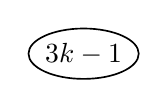
\begin{tikzpicture}[x=1cm, y=1cm, baseline=(e.base)]
\node (e) at (0,0) {$3k-1$};
\draw[line width=.6pt] (0,0) ellipse (.7cm and .32cm);
\end{tikzpicture}\par
\Unclear{GELFAND-P000140}{z2-overwritten-exponent}{The exponent on $z_2$ begins $3k$; its ending is heavily overwritten: $3k-1$ / another overwritten ending. Separately at the right, $3k-1$ is circled with an oval. The written exponent on $z_1$ is $3$.}
\end{GelfandAdjacentEvidence}


\begin{GelfandAdjacentEvidence}{GELFAND-P000140}{3}
\Unclear{GELFAND-P000140}{modulus-overwrite}{In the second line, the right bar and exponent at $|z_3|$ are heavily overwritten; $|z_3|^2$ is given with this qualification. Between $|z_4|^2$ and $|z_5|^2$ the sign resembles $+$ but is dense.}
\end{GelfandAdjacentEvidence}
\begin{GelfandAdjacentEvidence}{GELFAND-P000140}{4}

10 unk. and [crossed-out unread fragment] 3 eqns.
\Unclear{GELFAND-P000140}{cancelled-equation-count}{A short crossed-out fragment after “and”: a $7$-like sign and further dense strokes; the original content is unreadable.}
\end{GelfandAdjacentEvidence}

\underline{Milnor:} this is homeomorphic to $S^7$

\uwave{Hirzebruch:} for $k=1,2,\ldots,28$ there are different diff. structures there, and thereafter everything repeats periodically and these are all the Milnor spheres.

$S^{11}$ there are 992 of them and they are obtained by such equations.



\begin{GelfandAdjacentEvidence}{GELFAND-P000141}{1}
\SourcePage{GELFAND-P000141}{unlabelled}
\uuline{Bass} (Kazhdan\, [?])\quad \underline{rigidity of arithm. subgroups.}
\Unclear{GELFAND-P000141}{speaker-name}{The third letter of the Cyrillic surname between “Ka” and “dan” is a dense connected stroke: “Kazhdan” / “Kazdan”.}
\end{GelfandAdjacentEvidence}

\underline{$SL (n, Z)\subset SL (n, R)$ — a rigid subgroup,}

\begin{GelfandAdjacentEvidence}{GELFAND-P000141}{2}
[A short opening and a word before “every” are crossed out.]
\Unclear{GELFAND-P000141}{cancelled-introduction}{The initial crossed-out designation resembles “II.” / Cyrillic “Те.”; the following heavily cancelled word is unreadable.}
\end{GelfandAdjacentEvidence}

every deformation, (i.e. a map)
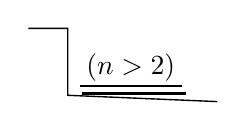
\begin{tikzpicture}[x=1cm, y=1cm, baseline=(d.base)]
\node (d) at (.8,.35) {$(n>2)$};
\draw[line width=.5pt] (-.5,.85) -- (0,.85) -- (0,0) -- (1.9,-.08);
\draw[line width=.5pt] (.15,.12) -- (1.45,.12);
\draw[line width=.9pt] (.18,.025) -- (1.5,.025);
\end{tikzpicture}
\begin{equation*}SL (n, Z)\times[0,1]\longrightarrow SL (n, R)\end{equation*}

which is continuous and a homomorphism for $\forall t\in[0,1]$, at $t=0$ it is the inclusion) is trivial, i.e. it is an inner automorphism with respect to $g (t)$ (a curve in the group)
\begin{equation*}\varphi (h\times t)=g (t)h\cdot g (t)^{-1},\qquad h\in SL (n, Z)\end{equation*}

Weil's theorem is proved only for the case when the quotient space is compact.

The prob. reduces to a problem about congruence subgrps. over a finite field.
(If there are two homomorphisms, it is unknown whether they can be joined)

\begin{GelfandAdjacentEvidence}{GELFAND-P000141}{3}
Existence of deformations — nontrivial
\begin{center}
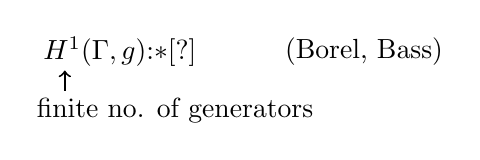
\begin{tikzpicture}[x=1cm, y=1cm]
\node at (0,0) {$H^1(\Gamma,\mathfrak g)\mathord{:}\mathord{*}\text{[?]}$};
\node at (3.1,0) {(Borel, Bass)};
\node at (.7,-.75) {finite no. of generators};
\draw[->,line width=.7pt] (-.7,-.5) -- (-.7,-.24);
\end{tikzpicture}
\end{center}
\Unclear{GELFAND-P000141}{cohomology-terminal}{After $H^1(\Gamma,\mathfrak g)$ are small colon-like and star-like strokes; their literal reading is not established. Below the expression is “finite no. of generators” with an upward arrow.}
\end{GelfandAdjacentEvidence}

$\mathfrak g$ — the Lie algebra.

In $\mathfrak g$ there is a lattice of integer matrices $L$. ($L$ — a lattice in the Lie algebra)
\begin{equation*}H^1(\Gamma,\mathfrak g)=H^1(\Gamma, L)\underset Z\otimes R\end{equation*}

Prove that $H^1(\Gamma, L)$ is finite,
It suffices to prove that $\exists\underset{\underline{\text{prime}}}{p}$ such that multiplication by $p$ is an epimorphism
\begin{gather*}
H^1(\Gamma, L)\overset p\longrightarrow H^1(\Gamma, L)\longrightarrow H^1(\Gamma, L/pL)\\
(\text{from }0\longrightarrow L\overset p\longrightarrow L\longrightarrow L/pL\longrightarrow0)
\end{gather*}

It suffices to prove that the right-hand term is $0$.

One can reduce the matter to the case when $\Gamma$ is finite: in place of $\Gamma$ — $\Gamma/[\Gamma_p,\Gamma_p]$, $\Gamma_p$ — the grp. of elems. congruent to $1$ modulo $p$.



\SourcePage{GELFAND-P000142}{6}
Thus, it suffices to prove that
\begin{equation*}H^1(\Gamma/\Gamma_p, L/pL)=0\end{equation*}
and everything reduces to fin. groups.
The same \uuline{Borel} an incredibly difficult proof.
\underline{Bass} — only for split ones.

\uuline{Smale} (Anosov)

\begin{flushright}
\begin{tikzpicture}[x=1cm, y=1cm, baseline=(p.base)]
\node (p) at (.35,.35) {$6$};
\draw[line width=.6pt] (0,.8) -- (0,0) -- (.9,0);
\end{tikzpicture}
\end{flushright}

\begin{GelfandAdjacentEvidence}{GELFAND-P000142}{1}
\uwave{Arnold.}\quad \uwave{$U$-system} \underline{(according to Anosov)}
\begin{equation*}g: H\text{[?]}\underset{\text{diff.}}{\longrightarrow}H\text{[?]},\end{equation*}
if
\Unclear{GELFAND-P000142}{manifold-letter}{The domain and range letters are written like $H$; $H$ / $M$. The precise definition below has $TM_x$. Beneath the arrow is “diff.”.}
\end{GelfandAdjacentEvidence}

there are 2 dirs.

\begin{GelfandAdjacentEvidence}{GELFAND-P000142}{2}
\SourceFigure{GELFAND-P000142}{directions-diagram}{Two separate intersections of horizontal and nearly vertical segments; a gap in the upper part of the first vertical stroke. There are no arrows or letter labels.\par\smallskip\centering{\color{black}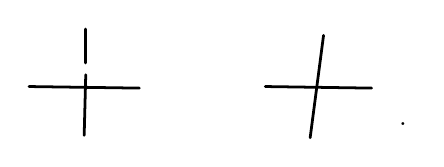
\begin{tikzpicture}[x=1cm, y=1cm, line width=1pt, line cap=round]
\draw (-.7,.02) -- (.7,0);
\draw (0,-.6) -- (.02,.17);
\draw (.02,.32) -- (.02,.75);
\draw (2.3,.02) -- (3.65,0);
\draw (2.87,-.63) -- (3.04,.67);
\node at (4.05,-.45) {.};
\end{tikzpicture}}}
\end{GelfandAdjacentEvidence}
\begin{GelfandAdjacentEvidence}{GELFAND-P000142}{3}

along the 1st it stretches\, [?], along the other it contracts ($\leq$, $\geq$ estimates on contraction and stretching)
\Unclear{GELFAND-P000142}{stretch-contraction}{The final letter of the contraction after “along the 1st” has dense joined strokes: Cyrillic “растяг.” / “растяж.”, both contractions of “stretching”. The contracted original is not expanded into a claimed exact Russian word.}
\end{GelfandAdjacentEvidence}

\begin{center}
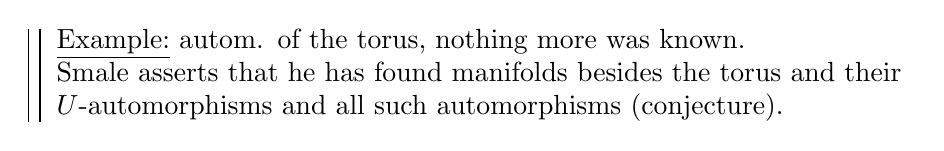
\begin{tikzpicture}[x=1cm, y=1cm]
\node[anchor=north west, inner sep=0pt, text width=.9\linewidth] (example) at (0,0) {\underline{Example:} autom. of the torus, nothing more was known.\par Smale asserts that he has found manifolds besides the torus and their $U$-automorphisms and all such automorphisms (conjecture).};
\draw[line width=.6pt] ([xshift=-2mm]example.north west) -- ([xshift=-2mm]example.south west);
\draw[line width=.6pt] ([xshift=-3.5mm]example.north west) -- ([xshift=-3.5mm]example.south west);
\end{tikzpicture}
\end{center}

\uwave{Precise def.:}\quad $\exists TM_x=X_x\oplus Y_x$, $\forall\xi\in X_x$, $g^*\xi\in X_{gx}$,
\par\noindent a Riem. metric exists
\begin{gather*}
|g^*\xi|<\theta|\xi|,\quad 0<\theta<1,\\
\forall\eta\in Y_x,\quad |g^*\eta|>\frac1\theta|\eta|.
\end{gather*}

\begin{GelfandAdjacentEvidence}{GELFAND-P000142}{4}
(this is a $V$\, [?]-cascade)
\Unclear{GELFAND-P000142}{u-v-designation}{The opening heading has $U$, whereas this sign resembles $V$: $V$-cascade / $U$-cascade.}
\end{GelfandAdjacentEvidence}

\uwave{Autom. of the torus} — eigendirections of the corresponding matrix.

\begin{GelfandAdjacentEvidence}{GELFAND-P000142}{5}
All
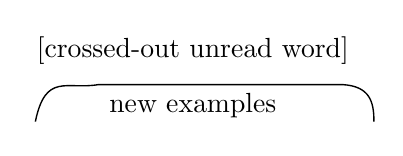
\begin{tikzpicture}[x=1cm, y=1cm, baseline=(cancel.base)]
\node (cancel) at (1.9,.55) {[crossed-out unread word]};
\node at (1.9,-.15) {new examples};
\draw[line width=.5pt] (-.1,-.35) .. controls (.03,.28) and (.3,.05) .. (.7,.12) -- (3.8,.12) .. controls (4.15,.1) and (4.2,-.1) .. (4.2,-.35);
\end{tikzpicture}
— a quotient of a nilp. group by a discrete subgroup. (nil-manifolds)
\Unclear{GELFAND-P000142}{cancelled-examples-word}{The crossed-out word after “All” has Cyrillic с/ю/д-like remnants; the original word is unreadable. The insertion “new examples” is visible beneath a spanning curved mark.}
\end{GelfandAdjacentEvidence}
\begin{GelfandAdjacentEvidence}{GELFAND-P000142}{6}

$G/\Gamma$, $G=$
\begin{center}
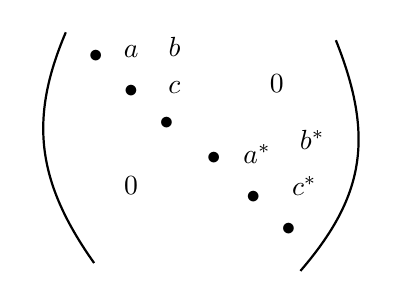
\begin{tikzpicture}[x=1cm, y=1cm]
\draw[line width=.8pt] (.12,2.95) .. controls (-.35,1.85) and (-.25,1.05) .. (.48,.02);
\draw[line width=.8pt] (3.55,2.85) .. controls (4.05,1.6) and (3.9,.85) .. (3.1,-.08);
\node at (.5,2.65) {$\bullet$};
\node at (.95,2.7) {$a$};
\node at (1.5,2.77) {$b$};
\node at (.95,2.2) {$\bullet$};
\node at (1.5,2.25) {$c$};
\node at (1.4,1.8) {$\bullet$};
\node at (2.8,2.3) {$0$};
\node at (.95,1) {$0$};
\node at (2,1.35) {$\bullet$};
\node at (2.55,1.4) {$a^*$};
\node at (3.25,1.58) {$b^*$};
\node at (2.5,.85) {$\bullet$};
\node at (3.15,1) {$c^*$};
\node at (2.95,.45) {$\bullet$};
\end{tikzpicture}
\end{center}
— of order 6
\Unclear{GELFAND-P000142}{nilpotent-matrix}{A matrix in round parentheses, six diagonal positions, two upper-triangular blocks. At the top $a, b$, below $c$; in the lower block $a^*, b^*, c^*$; two $0$ signs outside the blocks. The six dense diagonal marks are shown as dots: $1$ / black dots; their exact literal reading is not established.}
\end{GelfandAdjacentEvidence}
\begin{GelfandAdjacentEvidence}{GELFAND-P000142}{7}

\begin{gather*}
\Gamma=\left\{\begin{aligned}
a&=m+n\sqrt3,\qquad a^{*\text{[?]}}=m-n\sqrt3\\
b&=m'+n'\sqrt3,\qquad \vcenter{\hbox{\begin{tikzpicture}[x=1cm, y=1cm, baseline=0pt, line width=1pt]
\draw (0,.08) -- (.05,0);
\draw (.45,.08) -- (.47,.01);
\draw (.88,.07) -- (.92,.02);
\draw (1.35,.08) -- (1.39,.01);
\draw (1.82,.1) -- (1.88,.03);
\draw (2.23,.11) -- (2.22,.05) -- (2.27,.02);
\end{tikzpicture}}},\\
c&=m''+n''\sqrt3,
\end{aligned}\right\}
\end{gather*}
\underline{$G/\Gamma$ is compact.}
\par Dim. $3+3$
\par contract. and expand.
\Unclear{GELFAND-P000142}{lower-lattice-and-brace}{A short dense mark above the second $a$: a star / a stroke; $a^*$ is given with this qualification. Six short repetition strokes stand at the right of the $b$ line; their content is not expanded. An encompassing right brace. The horizontal rule beneath “$G/\Gamma$ is compact.” runs above “Dim. $3+3$”.}
\end{GelfandAdjacentEvidence}



\SourcePage{GELFAND-P000143}{unlabelled}
\underline{Anosov proper.}

Cascade — iterations of a diff. homeomorphism
(with continuous time — a flow)
Describe typical dynamical systems — cascades.
(an everywhere dense set, open)

\underline{Structurally stable flow} — passes to an equivalent one under a small $(C^1)$ perturbation.
(equiv. — differ by a diffeom.)

\uwave{2-dimensional case:} \underline{Andronov–Pontryagin thm.} — structurally stable systems are described (a finite number of “stable” cycles and singular points and saddle separatrices in general position — — do not intersect, do not coincide.) Their set is open, dense.

\uwave{Andronov–Pontryagin system.}

1. A fin. number of equilibria and periodic trajectories, all locally structurally stable (conditions on eigenvalues and multipliers)
(in the multidimensional case this is already nontriv.)

2. Separatrices in general position

\noindent\begin{tabular}{p{.47\linewidth}p{.47\linewidth}}
(Cond.,\newline Conditionally stable manifolds,\newline Asympt. bundles,\newline horospheres,\newline horocycles) & (Manifolds of incoming and outgoing —\newline — see Coddington and Levinson)
\end{tabular}

3. All trajectories as $t\longrightarrow\pm\infty$ tend to equilibria and periodic solutions.

\begin{GelfandAdjacentEvidence}{GELFAND-P000143}{1}
[Two lines are densely cancelled with straight and wavy strokes. Surviving fragments: $4)$ / $\forall$\, [?], “separatrices in general position”, “(do not intersect”, $2$\, [?], Cyrillic “собр.”; below, “this is not very” [unread ending].]
\Unclear{GELFAND-P000143}{cancelled-fourth-condition}{The initial cancelled sign resembles $4)$ / $\forall$; further surviving fragments are “separatrices in general position”, “(do not intersect”, a $2$-like sign and Cyrillic “собр.”; below, “this is not very” and a dense ending. The complete original statement is unreadable.}
\end{GelfandAdjacentEvidence}

\underline{4 assertions.}

\begin{GelfandAdjacentEvidence}{GELFAND-P000143}{2}
1. All A.–P. — structurally stable —

\begin{tikzpicture}[x=1cm, y=1cm, baseline=(q.base)]
\node (q) at (0,0) {?};
\draw[line width=.7pt] (0,0) ellipse (.32cm and .4cm);
\end{tikzpicture}
\begin{center}
\begin{tikzpicture}[x=1cm, y=1cm]
\node[anchor=north west, inner sep=0pt, text width=.52\linewidth] (claims) at (0,0) {2. All structurally stable — A.–P.\par 3. A.–P. are dense\par \sout{(Cyrillic дру\, [?]}\par 4. Structurally stable are dense};
\draw[line width=.7pt] ([xshift=3mm]claims.north east) -- ([xshift=3mm]claims.south east);
\draw[line width=.7pt] ([xshift=4.5mm]claims.north east) -- ([xshift=4.5mm]claims.south east);
\node[anchor=west, align=left] at ([xshift=10mm]claims.east) {Refuted\\by Smale.};
\end{tikzpicture}
\end{center}
\SourceFigure{GELFAND-P000143}{four-assertions}{After item 1, a hook-shaped question mark with a separate dot is circled. At the right of items 2–4 are two vertical rules and the words “Refuted by Smale”.}
\end{GelfandAdjacentEvidence}

\begin{GelfandAdjacentEvidence}{GELFAND-P000143}{3}
\Unclear{GELFAND-P000143}{cancelled-parenthesis}{A short cancelled parenthesis beneath item 3: Cyrillic “дру” / “друг” / unreadable.}
\end{GelfandAdjacentEvidence}



\SourcePage{GELFAND-P000144}{7}
\begin{flushright}
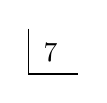
\begin{tikzpicture}[x=1cm, y=1cm, baseline=(p.base)]
\node (p) at (0,0) {$7$};
\draw[line width=.6pt] (-.28,.3) -- (-.28,-.28) -- (.35,-.28);
\end{tikzpicture}
\end{flushright}
\underline{Structurally stable system:} $\dot w=f (w)$.
\begin{equation*}
\forall\varepsilon\ \exists\delta,\quad \forall g,\quad \|g-f\|_{C^1}<\delta,
\end{equation*}
$\exists\varepsilon$-homeom., taking trajectories of $f$ to trajectories of $g$.

For a cascade: commutative diagram

($\exists\varepsilon$-homeom. $\chi$)

\begin{GelfandAdjacentEvidence}{GELFAND-P000144}{1}
\SourceFigure{GELFAND-P000144}{conjugacy-square}{Four $M$ nodes; $f$ above, $g$ below, both horizontal arrows point right, both vertical arrows down. At the left, $\chi$; at the right, a short $x$- / $\chi$-like sign.\par\smallskip\centering{\color{black}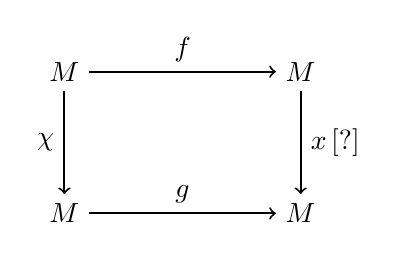
\begin{tikzpicture}[x=1cm, y=1cm]
\node (a) at (0,0) {$M$};
\node (b) at (3,0) {$M$};
\node (c) at (0,-1.8) {$M$};
\node (d) at (3,-1.8) {$M$};
\draw[->,line width=.7pt] (a) -- node[above] {$f$} (b);
\draw[->,line width=.7pt] (c) -- node[above] {$g$} (d);
\draw[->,line width=.7pt] (a) -- node[left] {$\chi$} (c);
\draw[->,line width=.7pt] (b) -- node[right] {$x\,[?]$} (d);
\end{tikzpicture}}}
\end{GelfandAdjacentEvidence}

(For flows it is natural to assume that the speed may change;
if this is forbidden, almost no structurally stable ones remain)

\uwave{A subset $b\vert$\, [?] of a manifold $M$ with a smooth cascade is called}
\uwave{a $U$-subset}
(\underline{hyperbolic} \underline{subset})

compact,

invariant,

\begin{GelfandAdjacentEvidence}{GELFAND-P000144}{2}
$\exists\Theta$ and a decomposition of the tangent bundle over $b\vert$\, [?] into a direct sum,
having the indicated properties. ($U$ $\ldots$)
\Unclear{GELFAND-P000144}{hyperbolic-set-symbol}{Subset designation: $b\vert$ / $b_1$ / another sign; a loop and a separate tall stroke. Repeated after “over”.}
\end{GelfandAdjacentEvidence}
\begin{GelfandAdjacentEvidence}{GELFAND-P000144}{3}

(the tangent space of the whole [unreadable short cancelled fragment] manifold is decomposed.)
\Unclear{GELFAND-P000144}{cancelled-tangent-word}{After “whole”, a short fragment is densely cancelled; the literal word cannot be read.}
\end{GelfandAdjacentEvidence}

\underline{Example:} 1) a hyperbolic equilibrium
(e.g. stable — — expanding — the whole space)

2) any $U$-system

3) There are examples when such a set is a torus, a Cantor set, etc.

\underline{Smale systems.}

\uwave{Nonwandering point.}

\begin{GelfandAdjacentEvidence}{GELFAND-P000144}{4}
\uwave{Wandering region:} $\exists n_0$ such that
\begin{equation*}
\forall n\ge n_0,\quad g^n U\cap U=\varphi\, [?]
\end{equation*}
\Unclear{GELFAND-P000144}{wandering-zero-and-headings}{At the right of the equality, a crossed oval with a long lower stroke: a $\varphi$- / $\varnothing$-like sign. “Smale systems” has a straight underline; the next two headings have wavy underlines.}
\end{GelfandAdjacentEvidence}

A point is called wandering if it has a wandering neighbourhood.

\begin{GelfandAdjacentEvidence}{GELFAND-P000144}{5}
A nonwandering point — a point that is not wandering, i.e.
\begin{equation*}
\forall U_p\ \forall n\quad \exists g\, [?]\in U_p,\quad m>n:\quad g^m q\in U_p.
\end{equation*}
\Unclear{GELFAND-P000144}{nonwandering-point-variable}{After $\exists$ is a $g$- / $q$-like letter; at the end, after $g^m$, a $q$-like letter.}
\end{GelfandAdjacentEvidence}

\underline{The set of nonwandering points is closed.} (denoted — $\Omega$)

\uwave{Smale} \uwave{system} (def)

1. $\Omega$ — hyperbolic.

\begin{GelfandAdjacentEvidence}{GELFAND-P000144}{6}
2. $\overline{\Gamma}=\Omega$
(periodic points are dense in $\Omega$ — nonwandering\, [?])
\Unclear{GELFAND-P000144}{bottom-parenthesis}{The explanation ends at the lower boundary: “— неблужд.” (nonwandering) / a similar contraction; dense strokes.}
\end{GelfandAdjacentEvidence}
\begin{GelfandAdjacentEvidence}{GELFAND-P000144}{7}

\uwave{$\Gamma_n$ — set of points of period $n$.}
\begin{equation*}
\vcenter{\hbox{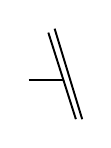
\begin{tikzpicture}[x=1cm, y=1cm]
\draw[line width=.7pt] (0,1.1) -- (.35,0);
\draw[line width=.7pt] (.08,1.15) -- (.43,0);
\draw[line width=.7pt] (-.25,.5) -- (.2,.5);
\end{tikzpicture}}}
\quad\Gamma=\bigcup_{n\ge1}\Gamma_n\, [?]\quad (g^n p=p)\, [?]
\end{equation*}
\Unclear{GELFAND-P000144}{periodic-definition-overwrite}{After the union sign, $\Gamma_n$-like signs, the opening parenthesis and $g$ are densely overwritten; the exponent is $n$-like. The original overwritten signs are undetermined. At the left are two slanting strokes with a short transverse stroke.}
\end{GelfandAdjacentEvidence}



\begin{GelfandAdjacentEvidence}{GELFAND-P000145}{1}
\SourcePage{GELFAND-P000145}{unlabelled}
It can happen that all points are nonwandering, but there are no periodic ones
(e.g. nil-flows\, [?])
\Unclear{GELFAND-P000145}{initial-example}{Faint parenthetical entry: “ниль-потоки” (nil-flows) / “нуль-потоки” (null-flows); the middle letter is not quite clear.}
\end{GelfandAdjacentEvidence}
\begin{GelfandAdjacentEvidence}{GELFAND-P000145}{2}

\underline{Conjectures.}
\begin{center}
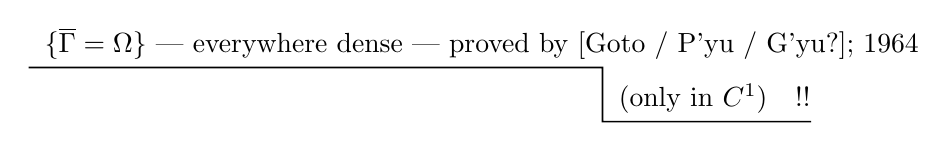
\begin{tikzpicture}[x=1cm, y=1cm]
\node[anchor=north west, inner sep=0pt, text width=.92\linewidth] (hyp) at (0,0) {$\{\overline{\Gamma}=\Omega\}$ — everywhere dense — proved by [Goto / P'yu / G'yu?]; 1964};
\node[anchor=north west, inner sep=0pt] (c1) at ([xshift=-.32\linewidth, yshift=-3mm]hyp.south east) {(only in $C^1$)\quad!!};
\draw[line width=.6pt] ([xshift=-2mm,yshift=-1mm]hyp.south west) -- ([xshift=-2mm,yshift=2mm]c1.north west) -- ([xshift=-2mm,yshift=-1mm]c1.south west) -- ([yshift=-1mm]c1.south east);
\end{tikzpicture}
\end{center}
\Unclear{GELFAND-P000145}{proof-name}{The surname before “; 1964”: “Гото” (Goto) / “Пью” (P'yu) / “Гью” (G'yu); faint lettering.}
\end{GelfandAdjacentEvidence}

\uwave{Smale systems are everywhere dense}

\begin{tikzpicture}[x=1cm, y=1cm, baseline=(q.base)]
\node (q) at (0,0) {?};
\draw[line width=.6pt] (0,0) ellipse (.3cm and .38cm);
\end{tikzpicture}

A great problem to which it is worth devoting one's life.

Apparently 2 follows from 1 (Prob. $70\%$),
so it suffices to prove that systems with hyperbolic $\Omega$ are dense.

\begin{GelfandAdjacentEvidence}{GELFAND-P000145}{3}
\underline{Theorem S. D. T.\, [?]} (Smale) (Spectral Decompositio\, [?] theorem)
\Unclear{GELFAND-P000145}{spectral-initials}{The first letter is $S$-shaped, the middle letter a looped $D$ / Cyrillic “Д”, the last $T$-shaped: S. D. T. / S.Д.T.}
\end{GelfandAdjacentEvidence}

\begin{GelfandAdjacentEvidence}{GELFAND-P000145}{4}
\Unclear{GELFAND-P000145}{spectral-title-terminal}{The word ending before “theorem”: Decompositio / Decomposition; the last visible sign is $o$- / $a$-like. An additional final $n$ is undetermined.}
\end{GelfandAdjacentEvidence}

\underline{on the structure of Smale systems.}
\begin{equation*}
\Omega=\bigcup_{i=1}^{k}\Omega_i
\end{equation*}
$\Omega_i$ — invariant, closed and topologically transitive.

All theorems follow from 1 alone.



\SourcePage{GELFAND-P000146}{unlabelled}
$12/\underline{\overline{\mathrm{IX}}}$ \underline{Gelfand sem.}

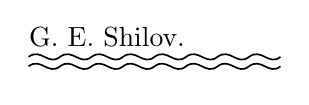
\begin{tikzpicture}[x=1cm, y=1cm, baseline=(sh.base)]
\node[anchor=south west, inner sep=0pt] (sh) at (0,.12) {G. E. Shilov.};
\draw[line width=.6pt] (0,0) .. controls (.16,.12) and (.25,-.12) .. (.4,0) .. controls (.56,.12) and (.65,-.12) .. (.8,0) .. controls (.96,.12) and (1.05,-.12) .. (1.2,0) .. controls (1.36,.12) and (1.45,-.12) .. (1.6,0) .. controls (1.76,.12) and (1.85,-.12) .. (2,0) .. controls (2.16,.12) and (2.25,-.12) .. (2.4,0) .. controls (2.56,.12) and (2.65,-.12) .. (2.8,0) .. controls (2.96,.12) and (3.05,-.12) .. (3.2,0);
\draw[line width=.6pt] (0,-.12) .. controls (.16,0) and (.25,-.24) .. (.4,-.12) .. controls (.56,0) and (.65,-.24) .. (.8,-.12) .. controls (.96,0) and (1.05,-.24) .. (1.2,-.12) .. controls (1.36,0) and (1.45,-.24) .. (1.6,-.12) .. controls (1.76,0) and (1.85,-.24) .. (2,-.12) .. controls (2.16,0) and (2.25,-.24) .. (2.4,-.12) .. controls (2.56,0) and (2.65,-.24) .. (2.8,-.12) .. controls (2.96,0) and (3.05,-.24) .. (3.2,-.12);
\end{tikzpicture}
\begin{equation*}
S=\{x\in H,\ |x|\le1\}
\end{equation*}
— the unit ball of a Hilbert space.

$L (S)$ — ring of all weakly continuous functions.
\begin{equation*}
L (S)\subset\overline R\subset C (S)
\end{equation*}
$C (S)$ — strongly continuous functions.

\begin{GelfandAdjacentEvidence}{GELFAND-P000146}{1}
\begin{equation*}
R=\{f ((e_1, x),\ldots,(e_n, x),|x-a_1|,\ldots,|x-a_m|),
\end{equation*}
$\overline R$ — closure
\Unclear{GELFAND-P000146}{ring-closing-brace}{After the long formula for $R$, a closing round parenthesis and a comma are visible; a closing brace for the initial $\{$ is not visible.}
\end{GelfandAdjacentEvidence}
\begin{GelfandAdjacentEvidence}{GELFAND-P000146}{2}

\begin{center}
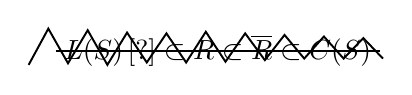
\begin{tikzpicture}[x=1cm, y=1cm]
\node[inner sep=0pt] (chain) at (0,0) {$L (S)\, [?]\subset R\subset\overline R\subset C (S)$};
\draw[line width=.7pt] ([xshift=-1mm]chain.west) -- ([xshift=1mm]chain.east);
\draw[line width=.7pt] (-2.4,-.18) -- (-2.15,.28) -- (-1.9,-.16) -- (-1.65,.26) -- (-1.4,-.18) -- (-1.15,.23) -- (-.9,-.15) -- (-.65,.22) -- (-.4,-.15) -- (-.15,.24) -- (.1,-.14) -- (.35,.22) -- (.6,-.12) -- (.85,.2) -- (1.1,-.1) -- (1.35,.18) -- (1.6,-.1) -- (1.85,.16) -- (2.1,-.1);
\end{tikzpicture}
\end{center}
\Unclear{GELFAND-P000146}{cancelled-inclusions}{The chain $L (S)\subset R\subset\overline R\subset C (S)$ is cancelled; the first letters and first inclusion sign are overwritten, and the beginning is not fully established.}
\end{GelfandAdjacentEvidence}

PIM of the ring $L (S)$ — the Hilbert ball

\begin{GelfandAdjacentEvidence}{GELFAND-P000146}{3}
PIM of $\overline R$ — a bicompact extension.
\begin{equation*}
M_\tau (f (x), z)\qquad M_\tau^*(f (x), z)
\end{equation*}
\Unclear{GELFAND-P000146}{mean-radius-symbol}{The mean's subscript is $\tau$- / $r$-like; the same looped sign occurs in the later limit formula and squared in its denominator.}
\end{GelfandAdjacentEvidence}

$e_1, e_2,\ldots, e_n,\ldots$ — an orthogonal basis, determining an increasing chain of subspaces $E_1\subset E_2\subset\ldots$
\begin{center}
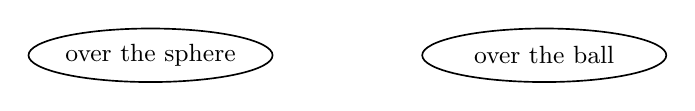
\begin{tikzpicture}[x=1cm, y=1cm]
\node[font=\small] (sphere) at (0,0) {over the sphere};
\node[font=\small] (ball) at (5,0) {over the ball};
\draw[line width=.6pt] (0,0) ellipse (1.55cm and .34cm);
\draw[line width=.6pt] (5,0) ellipse (1.55cm and .34cm);
\end{tikzpicture}
\end{center}
The means — the limit of finite-dimensional ones. If they exist, they are equal.

The means are defined on $\overline R$.

(For $R$, one can simply write down formulas).

$M_\tau$ — a multiplicative functional. This is a max ideal, but it is not a value at a point, but a value in bicompact extensions.

\begin{GelfandAdjacentEvidence}{GELFAND-P000146}{4}
From the point $z$, lines $M_\tau (z)$ are drawn in the space of max ideals.
\begin{equation*}
\Delta f (z)=\lim_{\tau\to0}\frac{M_\tau[f (x), z]-f (z)}{\tau^2}.
\end{equation*}
\begin{flushright}
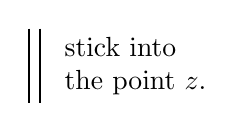
\begin{tikzpicture}[x=1cm, y=1cm]
\node[anchor=west, align=left, inner sep=0pt] (note) at (0,0) {stick into\\the point $z$.};
\draw[line width=.7pt] ([xshift=-3mm,yshift=1mm]note.north west) -- ([xshift=-3mm,yshift=-1mm]note.south west);
\draw[line width=.7pt] ([xshift=-4.5mm,yshift=1mm]note.north west) -- ([xshift=-4.5mm,yshift=-1mm]note.south west);
\end{tikzpicture}
\end{flushright}
\Unclear{GELFAND-P000146}{limit-radius-repeat}{The looped sign in $M_\tau$, below the limit and in $\tau^2$ is $\tau$ / $r$ / an undetermined letter. At the right of the formula are two vertical rules and “stick into the point $z$”.}
\end{GelfandAdjacentEvidence}

\underline{This is a first-order operator!!}
\begin{equation*}
\Delta (fg)=f\cdot\Delta g+(\Delta f)g
\end{equation*}

\underline{Dirichlet problem.}

$\Sigma$ — a $\underset{\text{(weak)}}{\text{closed surface}}$ (star-shaped)

\begin{GelfandAdjacentEvidence}{GELFAND-P000146}{5}
\SourceFigure{GELFAND-P000146}{dirichlet-surface}{An irregular rounded closed contour with $\Sigma$ at the upper right; seven radiating strokes, with small gaps at the centre. Several pass beyond the contour, the lower-left one ends inside; the left stroke bends before the centre. The lower-right stroke thickens at the contour; a separate arrowhead / point is undetermined.\par\smallskip\centering{\color{black}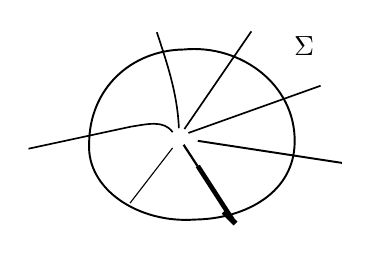
\begin{tikzpicture}[x=1cm, y=1cm]
\draw[line width=.7pt] (-1.18,-.12) .. controls (-1.18,.58) and (-.65,1.07) .. (.02,1.08) .. controls (.75,1.15) and (1.44,.63) .. (1.43,-.09) .. controls (1.43,-.72) and (.83,-1.07) .. (.16,-1.08) .. controls (-.56,-1.13) and (-1.21,-.69) .. (-1.18,-.12) -- cycle;
\draw[line width=.6pt] (-.04,.08) .. controls (-.06,.54) and (-.2,.93) .. (-.32,1.3);
\draw[line width=.6pt] (.03,.07) -- (.88,1.31);
\draw[line width=.6pt] (.08,.02) -- (1.76,.62);
\draw[line width=.7pt] (.2,-.08) -- (2.03,-.36);
\draw[line width=.8pt] (.02,-.13) -- (.64,-1.08);
\draw[line width=1.7pt] (.2,-.4) -- (.64,-1.08);
\draw[line width=2pt] (.53,-.98) -- (.68,-1.13);
\draw[line width=.4pt] (-.12,-.17) -- (-.66,-.87);
\draw[line width=.6pt] (-.12,.03) .. controls (-.23,.19) and (-.45,.13) .. (-.65,.1) -- (-1.95,-.18);
\node at (1.55,1.12) {$\Sigma$};
\end{tikzpicture}}}
\end{GelfandAdjacentEvidence}

\begin{gather*}
\Delta u (x)=0,\\
u (x)|_{x=\sigma}=f (\sigma)
\end{gather*}



\SourcePage{GELFAND-P000147}{10}
\begin{flushright}
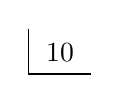
\begin{tikzpicture}[x=1cm, y=1cm, baseline=(p.base)]
\node (p) at (0,0) {$10$};
\draw[line width=.6pt] (-.4,.3) -- (-.4,-.28) -- (.4,-.28);
\end{tikzpicture}
\end{flushright}
There is uniqueness and continuous dependence for $f\in\overline R$ and surfaces of the form
\begin{equation*}
\sum_{k=m+1}^{\infty}\xi_k^2=\varphi (\xi_1,\ldots,\xi_m)
\end{equation*}

\begin{GelfandAdjacentEvidence}{GELFAND-P000147}{1}
(surface of rotation) about a subspace [unreadable short cancelled fragment] of finite codimension.
\Unclear{GELFAND-P000147}{cancelled-margin}{Before “of finite codimension”, a short fragment is densely cancelled; the literal word is undetermined.}
\end{GelfandAdjacentEvidence}

and bounded curvature.

The solution formula — the angular mean of the boundary functional.

$\Delta u=g\in\overline R$ — also explicit

Next, $\Delta u=\varphi (x, u (x))$ is solved by the fixed-point method.

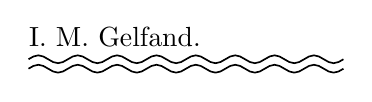
\begin{tikzpicture}[x=1cm, y=1cm, baseline=(gh.base)]
\node[anchor=south west, inner sep=0pt] (gh) at (0,.15) {I. M. Gelfand.};
\draw[line width=.6pt,domain=0:4,samples=65] plot (\x,{.05*sin(720*\x)});
\draw[line width=.6pt,domain=0:4,samples=65] plot (\x,{-.12+.05*sin(720*\x)});
\end{tikzpicture}

\begin{GelfandAdjacentEvidence}{GELFAND-P000147}{2}
$u=(u_1,\ldots, u_m\, [?])$
\Unclear{GELFAND-P000147}{component-count-index}{The last component subscript has a dense $m$- / $n$-like shape; below, $n=1$ and $n=2$ are written separately.}
\end{GelfandAdjacentEvidence}

\begin{equation*}
\frac{\partial u}{\partial t}=A (u)\frac{\partial u}{\partial x}
\end{equation*}
Hyperbolic (at $\forall$ point, $A (u)$ has real eigenvalues)

Is there uniqueness? Shock waves — the solution may be nonunique.

$n=1$ — always uniqueness if $f (u)$ is convex

\begin{GelfandAdjacentEvidence}{GELFAND-P000147}{3}
Hydrodynamic equations — [cancelled: “nonunique” / “may” / unreadable] uniqueness too. ($n=2$)
\Unclear{GELFAND-P000147}{hydro-cancelled-word}{Before “uniqueness too”, a word is cancelled: “может” (may) / “неод.” (nonunique) / another short fragment; the cancellation crosses the letters.}
\end{GelfandAdjacentEvidence}

In the general case it is unclear \dashuline{where there is uniqueness and where there is not}.

\begin{GelfandAdjacentEvidence}{GELFAND-P000147}{4}
Magn.\, [?] hydrodyn. — uniqueness too.
\Unclear{GELFAND-P000147}{hydro-prefix}{The first abbreviation before “hydrodyn.”: “Магн.” (Magn.) / “Мал.” (Mal.); the strokes after “Ма” are joined.}
\end{GelfandAdjacentEvidence}

\uwave{A purely mathematical question:} at $\forall$ point $u$, draw the eigenvectors — 3 families of lines — — characteristics.

Convexity: possibly, growth of $\lambda$ along the characteristics

Better:
\begin{equation*}
\frac{\partial u}{\partial t}=\frac{\partial f (u)}{\partial x}
\end{equation*}
(divergence form)

There is work by Godunov, but it concerns a narrow class of systems.

When is there uniqueness upon adding viscosity:
\begin{equation*}
\frac{\partial u}{\partial t}=A\frac{\partial u}{\partial x}+\varepsilon\frac{\partial^2u}{\partial x^2}\quad?
\end{equation*}

\begin{GelfandAdjacentEvidence}{GELFAND-P000147}{5}
This reduces to the [unreadable cancelled word] question of ordinary differential equations.
\Unclear{GELFAND-P000147}{cancelled-final-word}{In the source, between “к” (to) and “вопросу” (question), a densely cancelled word with a looped lower stroke; the literal reading is undetermined.}
\end{GelfandAdjacentEvidence}



\SourcePage{GELFAND-P000148}{unlabelled}
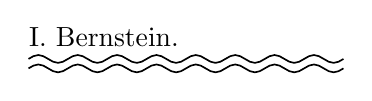
\begin{tikzpicture}[x=1cm, y=1cm, baseline=(bh.base)]
\node[anchor=south west, inner sep=0pt] (bh) at (0,.15) {I. Bernstein.};
\draw[line width=.6pt,domain=0:4,samples=65] plot (\x,{.05*sin(720*\x)});
\draw[line width=.6pt,domain=0:4,samples=65] plot (\x,{-.12+.05*sin(720*\x)});
\end{tikzpicture}

Part of what \underline{Atiyah} spoke about.

$g$ — a compact Lie group. $R_g$ — the ring of finite-dimensional representations
(direct sum, tensor product and formal differences), commutative.

An embedding
\begin{equation*}
R_g\longrightarrow K (B_g)
\end{equation*}
$B_g$ — the classifying space,
$K$ — the $K$-functor.

A representation corresponds to a vector bundle on $B_g$ (associated).


\begin{tikzpicture}[x=1cm, y=1cm, baseline=(ci.base)]
\node (ci) at (0,0) {$\mathrm{I.}$};
\draw[line width=.7pt] (0,0) ellipse (.33cm and .36cm);
\end{tikzpicture}
If the ring $R_g$ is completed at the ideal of representations of dimension zero, there will be an isomorphism
\begin{equation*}
\widehat R_g\longrightarrow k (B_g)
\end{equation*}
(The dimension of an element of the form of a difference of two representations — the difference of their dimensions)

\underline{Example.}
\begin{equation*}
g=S^1,\qquad R_{S^1}=\sum_{i=-\infty}^{+\infty}n_i x^i,
\end{equation*}
$n_i$ — integers, finitely many nonzero.

The ideal is generated by the element $x-1=y$.

\begin{equation*}
\widehat R_{S^1}=Z[[y]]
\end{equation*}
(formal power series)

Only positive powers
\begin{equation*}
\left (\frac1{1-y}=1+y+y^2+\ldots\right)
\end{equation*}
\begin{gather*}
B_g=CP^\infty,\\
k (CP^\infty)=\lim K (CP^n).
\end{gather*}

On $CP^n$, the canonical bundle (fibre $CP^1$), total space $CP^{n+1}$.

Every element of $K (CP^n)$ is $\underline{P}(x-1)$.

\begin{GelfandAdjacentEvidence}{GELFAND-P000148}{1}
Precisely
\begin{equation*}
K (CP^n)\cong\, [?]\ P (x)/(x-1)^{n+1}.
\end{equation*}
\Unclear{GELFAND-P000148}{quotient-relation}{The relation sign has a wavy upper stroke and lower horizontal strokes: $\cong$ / $\simeq$ / an overwritten sign. The numerator has a $P$-shaped letter.}
\end{GelfandAdjacentEvidence}

Next time, a lecture by Minlos on statistical physics.



\SourcePage{GELFAND-P000149}{unlabelled}
19/$\overline{\underline{\mathrm{IX}}}$. \uwave{Gelfand sem.}

\uwave{I. Bernstein} (continuation).

$K (B_g)$ is defined as follows:

Let
\begin{gather*}
(B_g)_1\longrightarrow (B_g)_2\longrightarrow\ldots
\end{gather*}
be the skeleta of the corresponding dimensions
\begin{gather*}
K_1\longleftarrow K_2\longleftarrow\ldots
\end{gather*}
One must take the projective limit.

\begin{GelfandAdjacentEvidence}{GELFAND-P000149}{1}
The $K$-functor of a finite polyhedron is defined in the usual way
(ring [overwritten: $K$-like sign, ?] bundl.[?])
\sout{[unread long entry]}) .
\begin{center}
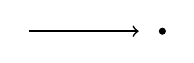
\begin{tikzpicture}[x=1cm, y=1cm]
\draw[->,line width=.6pt] (0,0)--(1.4,0);
\fill (1.7,0) circle (.045cm);
\end{tikzpicture}
\end{center}
\Unclear{GELFAND-P000149}{cancelled-definition}{After “ring”, an overwritten $K$-like sign and a “рассл.”-like abbreviation. Then dense cancellation with lower strokes and another closing parenthesis; a rightward arrow and dot below the beginning of the cancellation. The literal reading of the cancelled ending is not established.}
\end{GelfandAdjacentEvidence}
\begin{GelfandAdjacentEvidence}{GELFAND-P000149}{2}

\uwave{Question of I. M. Gelfand.} generalize the notion of the $K$-functor
and classifying space so that the theorem remains valid also for locally
compact Lie groups. (the left-hand side makes sense) —
— one must also use infinite-dimensional representations.
\SourceFigure{GELFAND-P000149}{question-parenthesis}{A wavy line below the heading. The faint parenthesis reads “the left-hand side makes sense”; the abbreviation at the right of the preceding line is “лок.”.}
\end{GelfandAdjacentEvidence}
\begin{GelfandAdjacentEvidence}{GELFAND-P000149}{3}

Dimension — a factor[?] in the Plancherel formula.
\begin{center}
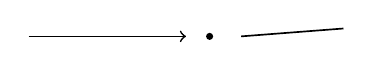
\begin{tikzpicture}[x=1cm, y=1cm]
\draw[->,line width=.6pt] (0,0)--(2,0);
\fill (2.3,0) circle (.045cm);
\draw[line width=.6pt] (2.7,0)--(4,.1);
\end{tikzpicture}
\end{center}
\Unclear{GELFAND-P000149}{plancherel-comparison}{The joined word after the dash: “factor” / “exponent” / unclear entry. Below it, a long rightward arrow, a dot and a short slightly rising stroke.}
\end{GelfandAdjacentEvidence}

Let $X$ be a $g$-space
(i.e. there is a map $g\times X\longrightarrow X$,
continuous in both arguments, and there is
an action of $g$ on $X$)

\begin{GelfandAdjacentEvidence}{GELFAND-P000149}{4}
$K_g (X\, [?])$ — the $K_g$[?]-functor.
\Unclear{GELFAND-P000149}{functor-index-placement}{At the second $K$, small loop-shaped strokes stand to the right, above and below: a $K_g$ / $K^g$ / $K_g^0$-like entry; a separate $0$ is not established. In the parentheses of the first $K_g$, an $X$-like letter is densely overwritten.}
\end{GelfandAdjacentEvidence}

A $g$-bundle $E\overset p\longrightarrow X$ — a vector bundle, then $E$ ...
— a $g$-space, $g$ acts compatibly with $p$.
In the fibres $g$ must preserve the linear structure.

In the usual way, sum and tensor product are defined and
formal differences are introduced.

\underline{Example.} $K_g$ — the functor of a point —
— linear spaces with representations of $g$,
this will be exactly $R_g$.

\begin{GelfandAdjacentEvidence}{GELFAND-P000149}{5}
\sout{[Cyrillic Н-like beginning, ?]...}
\Unclear{GELFAND-P000149}{cancelled-generalization}{Before “Generalization”, a short cancelled fragment with a Cyrillic Н-like beginning; the remaining letters are not established.}
\end{GelfandAdjacentEvidence}

\underline{Generalization.} Instead of a point — a $g$-space $X$.

The left-hand side $K_g (X)$ — already generalized.

\begin{GelfandAdjacentEvidence}{GELFAND-P000149}{6}
\begin{center}
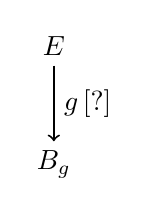
\begin{tikzpicture}[x=1cm, y=1cm]
\node (be) at (0,1.5) {$E$};
\node (bb) at (0,0) {$B_g$};
\draw[->,line width=.7pt] (be.south)--node[right] {$g\,[?]$} (bb.north);
\end{tikzpicture}
\end{center}
$E$ — a $g$-space ($g$ acts on the right).
\Unclear{GELFAND-P000149}{bottom-bundle}{Below, $E$ over $B_g$, a downward arrow and a small $g$-like loop-shaped sign to its right; the exact reading of the label is not established.}
\end{GelfandAdjacentEvidence}



\clearpage

\begin{GelfandAdjacentEvidence}{GELFAND-P000150}{1}
\SourcePage{GELFAND-P000150}{14}
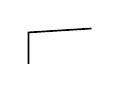
\begin{tikzpicture}[x=1cm, y=1cm, baseline=0pt]
\draw[line width=.6pt] (0,0)--(0,.4)--(.8,.45);
\end{tikzpicture}
\hfill\begin{tikzpicture}[x=1cm, y=1cm, baseline=(pn.base)]
\node (pn) at (.35,.35) {$14$};
\draw[line width=.6pt] (0,.85)--(0,0)--(1.05,0);
\end{tikzpicture}

Let $X$ be a $G\, [?]$-space. Introduce the space $X_G=E\times_G X$
(in $E\times X$, the orbits of the group $G$ are identified).
If $X$ is a point, then $X_G\cong B_G$ — Grassmann.

\Unclear{GELFAND-P000150}{group-glyph}{The loop-shaped group sign and its repeated indices: $G$ / $g$ / $\mathcal G$; rendered as $G$ with this qualification.}
\end{GelfandAdjacentEvidence}

\uuline{Theorem.} (a generalization of the one formulated at the beginning)
\begin{equation*}
\widehat K_G (X)\overset{\sim}{\longrightarrow}K (X_G).
\end{equation*}
There is a map $K_G (*)\longrightarrow K_G (X)$, so $K_G (X)$ —
— a module over $R_G$. Completion is taken with respect to the ideal $J$
of the ring $R_G$.

An exact def. can also be given as follows:
\begin{equation*}
\widehat K_G (X)=K_G (X)\underset{R_G}{\otimes}\widehat R_G.
\end{equation*}
\begin{center}
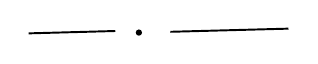
\begin{tikzpicture}[x=1cm, y=1cm]
\draw[line width=.7pt] (0,0)--(1.1,.03);
\fill (1.4,.01) circle (.04cm);
\draw[line width=.7pt] (1.8,.02)--(3.3,.06);
\end{tikzpicture}
\end{center}
1. \dashuline{Reduction to the unitary group $U$.}

Let $G\subset U$.
Then $K_G (X)=K_U (U\times_G X)$.

The action of $G$ on $U$: $g: u\longrightarrow ug^{-1}$.
On $U\times_G X$, $U$ acts on the left.
Moreover, $X_G=(U\times_G X)_U$.
\begin{flushright}
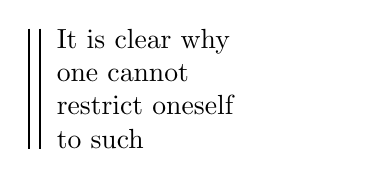
\begin{tikzpicture}[x=1cm, y=1cm]
\node[anchor=north west, inner sep=0pt, text width=.30\linewidth] (sidebar) at (0,0) {It is clear why\par one cannot\par restrict oneself\par to such};
\draw[line width=.7pt] ([xshift=-2mm]sidebar.north west)--([xshift=-2mm]sidebar.south west);
\draw[line width=.7pt] ([xshift=-3.5mm]sidebar.north west)--([xshift=-3.5mm]sidebar.south west);
\end{tikzpicture}
\end{flushright}

2. \dashuline{Reduction to the torus case.}

\begin{GelfandAdjacentEvidence}{GELFAND-P000150}{2}
(For the torus it holds, since for the circle verif.\, [?] directly.)
\Unclear{GELFAND-P000150}{torus-parenthesis}{After “окр.” (“circle”), a contraction resembling Cyrillic “пров.” / “пр-в.”; its middle strokes are joined. The parenthesis contains “непосредств.” (“directly”).}
\end{GelfandAdjacentEvidence}
\begin{GelfandAdjacentEvidence}{GELFAND-P000150}{3}

\sout{[unread cancelled sign]}.
\Unclear{GELFAND-P000150}{cancelled-torus-number}{Before $T\subset U$, a short number-like sign is densely cancelled; its original reading is not established. A separate dot at the right.}
\end{GelfandAdjacentEvidence}
\begin{GelfandAdjacentEvidence}{GELFAND-P000150}{4}

$T\subset U$, $T$ is a maximal torus in $U$.
\begin{center}
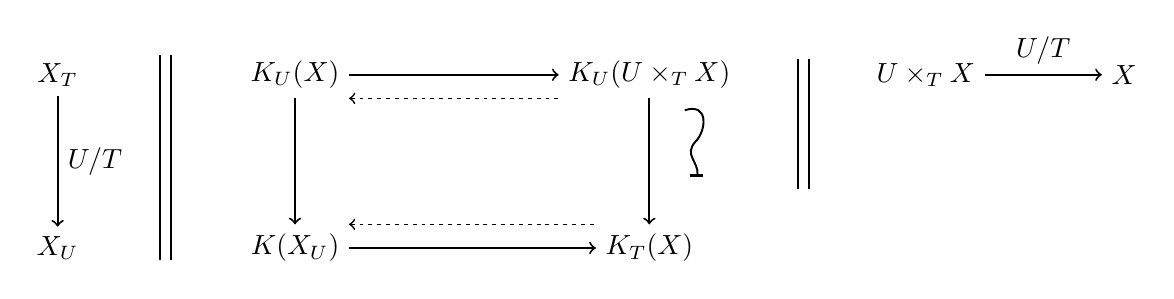
\begin{tikzpicture}[x=.9cm, y=1cm]
\node (fibreT) at (.35,0) {$X_T$};
\node (fibreU) at (.35,-2.2) {$X_U$};
\draw[->,line width=.7pt] (fibreT.south)--node[right] {$U/T$} (fibreU.north);
\draw[line width=.7pt] (1.8,.25)--(1.8,-2.35);
\draw[line width=.7pt] (1.95,.25)--(1.95,-2.35);
\node (topA) at (3.7,0) {$K_U (X)$};
\node (topB) at (8.7,0) {$K_U (U\times_T X)$};
\node (bottomA) at (3.7,-2.2) {$K (X_U)$};
\node (bottomB) at (8.7,-2.2) {$K_T (X)$};
\draw[->,line width=.7pt] (topA.east)--(topB.west);
\draw[<-,dash pattern=on 1.4pt off 1.8pt,line width=.6pt] ([yshift=-3mm]topA.east)--([yshift=-3mm]topB.west);
\draw[->,line width=.7pt] (bottomA.east)--(bottomB.west);
\draw[<-,dash pattern=on 1.4pt off 1.8pt,line width=.6pt] ([yshift=3mm]bottomA.east)--([yshift=3mm]bottomB.west);
\draw[->,line width=.7pt] (topA.south)--(bottomA.north);
\draw[->,line width=.7pt] (topB.south)--(bottomB.north);
\draw[line width=.7pt] (9.2,-.45) .. controls (9.55,-.35) and (9.5,-.72) .. (9.35,-.85) .. controls (9.18,-1.02) and (9.4,-1.1) .. (9.38,-1.28);
\draw[line width=1.3pt] (9.28,-1.28)--(9.45,-1.28);
\draw[line width=.7pt] (10.8,.2)--(10.8,-1.45);
\draw[line width=.7pt] (10.95,.2)--(10.95,-1.45);
\node (projectionA) at (12.6,0) {$U\times_T X$};
\node (projectionB) at (15.4,0) {$X$};
\draw[->,line width=.7pt] (projectionA.east)--node[above] {$U/T$} (projectionB.west);
\end{tikzpicture}
\end{center}
\SourceFigure{GELFAND-P000150}{torus-diagrams}{At the left, $X_T\longrightarrow X_U$ downward with $U/T$. Two double vertical rules separate three parts. In the square, $K_U (X)$ and $K_U (U\times_T X)$ above, $K (X_U)$ and $K_T (X)$ below; solid horizontal arrows rightward, dashed arrows backward, both vertical arrows downward. To the right of the right vertical arrow, a question-like hook with a thickened base; a separate dot cannot be distinguished. Separately at the right, $U\times_T X\longrightarrow X$ with $U/T$ above the arrow.}
\end{GelfandAdjacentEvidence}

The upper arrow is a map into a direct \underline{summand} (i.e. there exists
\begin{tikzpicture}[x=1cm, y=1cm, baseline=(inverse.base)]
\node[anchor=base west, inner sep=0pt] (inverse) at (0,0) {„inverse};
\node[anchor=south west, inner sep=0pt, font=\small] at (0,.34) {(and odd\, [?])};
\end{tikzpicture}
is constructed above and below functorially. \underline{„inverse“})

\begin{GelfandAdjacentEvidence}{GELFAND-P000150}{5}
Hence the left arrow is also an isomorphism.
\Unclear{GELFAND-P000150}{inverse-insert}{Above the first “inverse”, a parenthesized insertion: Cyrillic “и нечётное” / “и нечётн.” / “и нечёткое” / “и нечётная” / a dense contraction after “and”. The middle and final strokes are not securely separable. “summand” and the last “inverse” are underlined.}
\end{GelfandAdjacentEvidence}



\begin{GelfandAdjacentEvidence}{GELFAND-P000151}{1}
\SourcePage{GELFAND-P000151}{unlabelled}
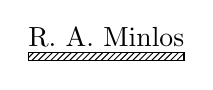
\begin{tikzpicture}[x=1cm, y=1cm, baseline=(minlos.base)]
\node[inner sep=0pt, outer sep=0pt] (minlos) {R. A. Minlos};
\begin{scope}
\clip ([yshift=-2pt]minlos.south west) rectangle ([yshift=-5pt]minlos.south east);
\foreach \hatch in {-3,-2.92,...,6} {
\draw[line width=.35pt] (\hatch,-.35)--++(.45,.45);
}
\end{scope}
\draw[line width=.5pt] ([yshift=-2pt]minlos.south west) rectangle ([yshift=-5pt]minlos.south east);
\end{tikzpicture}.


A \uwave{phys. system} is descr. by a set of states $\mathcal L_\sigma\, [?]$ and
a function $H (a)$ on \sout{[unreadable sign]}, which is called the Hamiltonian fn.
(a real-valued fn.). — the pair $(\mathcal L\, [?]; H (a), a\in\mathcal L_\sigma\, [?])$.
\Unclear{GELFAND-P000151}{cancelled-state-glyph}{After “on” a letter with an upper loop and a lower stroke is densely crossed out; the original reading is not established.}
\end{GelfandAdjacentEvidence}

\begin{GelfandAdjacentEvidence}{GELFAND-P000151}{2}
\Unclear{GELFAND-P000151}{state-glyph}{The state space: $\mathcal L_\sigma$ / a single handwritten $\mathcal G$-like letter; the right loop may be part of the letter or a separate $\sigma$. At the start of the pair a separate subscript is not established.}
\end{GelfandAdjacentEvidence}


\underline{3 types.}

1. \uwave{Classical system} — tuples
\begin{equation*}
(p_1,\ldots, p_N, x_1,\ldots, x_N)
\end{equation*}
All $p_i$ independently range over $\mathbb R^\nu$ (in physics $\mathbb R^3$) —
— the set of momenta.

\begin{GelfandAdjacentEvidence}{GELFAND-P000151}{3}
All $x_i$ range over a region \sout{[unreadable sign]}
$\Omega\subset\mathbb R^\nu$, called the \uwave{vessel} (the reg. is bounded).
\Unclear{GELFAND-P000151}{cancelled-vessel-glyph}{Before $\Omega$ there is a short densely crossed-out sign; the original reading is not established.}
\end{GelfandAdjacentEvidence}

The tuple $x_i$ — configurations of the particles
\begin{equation*}
(\underbrace{p_1,\ldots, p_N}_{\mathbb R^{N\nu}},\underbrace{x_1,\ldots, x_N}_{\Omega^N})
\end{equation*}


Notation (will sometimes be consid.)
\begin{equation*}
(\Omega_\delta)^N:\quad |x_i-x_j|>\delta
\end{equation*}
(the particles — “hard” balls)

This is the set of states.


\uwave{Hamiltonian fn.}:
\begin{equation*}
H (a)=\frac1{2m}\sum|p_i|^2+V (x_1,\ldots, x_N),\qquad m>0
\end{equation*}
$V$ is called the potential energy.

In what follows we consid. only fns. $V$ of the form

\begin{equation*}
V (x_1,\ldots, x_N)=\sum_{i\ne j}U (|x_i-x_j|)
\end{equation*}
(a system with pairwise interaction)

\begin{GelfandAdjacentEvidence}{GELFAND-P000151}{4}

$U (r)\, [?]$ — the potential — is def. either for $r>0$, or
for $r>\delta$.
\begin{equation*}
\{\mathcal L_\sigma{}_{\Omega, N}\, [?], H_{m, U (r)}\}
\end{equation*}
\Unclear{GELFAND-P000151}{state-parameter-glyph}{The loop-shaped state-space sign with its right loop recurs inside the brace; $\Omega, N$ are clearly visible below. The rendering of the principal sign as $\mathcal L_\sigma$ remains provisional.}
\end{GelfandAdjacentEvidence}
\begin{GelfandAdjacentEvidence}{GELFAND-P000151}{5}

$\Omega$ — the vessel, $N$ — the number of particles, $m$ — the mass, $U (r)\, [?]$ —
$\longrightarrow$ potential energy.
\Unclear{GELFAND-P000151}{potential-argument-glyph}{The letter in $U (r)$ and before $>0$, $>\delta$ has a short loop-shaped top and a lower stroke to the right: $r$ / a $\tau$-like handwritten sign. The rendering as $r$ is provisional; the repetitions appear in the original fragments.}
\end{GelfandAdjacentEvidence}



\begin{GelfandAdjacentEvidence}{GELFAND-P000152}{1}
\SourcePage{GELFAND-P000152}{15}
\hfill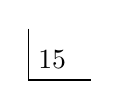
\begin{tikzpicture}[x=1cm, y=1cm, baseline=(pn.base)]
\node (pn) at (.3,.25) {$15$};
\draw[line width=.6pt] (0,.65)--(0,0)--(.8,0);
\end{tikzpicture}

\uwave{Identical sys.} — differ either in the number of particles or in the vessel.
(the same — mass and potential)

$\delta$ — is contained in $U (r)\, [?]$.


2. \uwave{Configurational system}.

Obt. from the preceding one.
A state — $(x_1,\ldots, x_N)$ — the region $\Omega^N$ or its
subregion $(\Omega_\delta)^N$.
\begin{equation*}
H (a)=\sum_{i\ne j}U (|x_i-x_j|)
\end{equation*}
— without kinetic energy.
\begin{equation*}
(\mathcal L_\sigma{}_{\Omega, N}\, [?], H^N_{U (r)})
\end{equation*}
\Unclear{GELFAND-P000152}{state-glyph}{The state-space letter repeats the loop-shaped sign: $\mathcal L_\sigma$ / a single $\mathcal G$-like letter; the right loop may be part of the letter or a separate $\sigma$. Below are $\Omega, N$.}
\end{GelfandAdjacentEvidence}

System 1 reduces to system 2. (see below).


\par\noindent\begin{minipage}[t]{\linewidth}
3. \uwave{Discrete model system}.

In $R^\nu$ a cubic lattice, $\Omega$ — a subset of it.
A state — a tuple of $N$ lattice sites $(x_1,\ldots, x_N)$,
in which no two are equal.
\end{minipage}\par

$U (x)$ — an even function on the lattice.
\begin{equation*}
H (a)=\sum_{i\ne j}U (x_i-x_j)
\end{equation*}
(Isotropy, e.g. — spherical symm. — is not justified here)


The results of stat. physics depend only on the qualit.
properties of $U (r)\, [?]$, but physicists use only the potential
\begin{equation*}
U (r)=\frac a{r^{12}}-\frac b{r^6},\qquad
\begin{gathered}a>0\mathstrut\\ b>0\end{gathered}
\end{equation*}
What matters to us is the growth at $0$ and the decay at $\infty$.

\begin{GelfandAdjacentEvidence}{GELFAND-P000152}{2}
\SourceFigure{GELFAND-P000152}{potential-graph}{The vertical axis has an upward arrow; no horizontal arrow is established. Neither axis has letters. The branch comes from above to the right of the vertical axis, crosses the horizontal, forms a negative well and approaches the horizontal from below. The upper end of the branch is thick, with short lateral strokes; a separate arrow meaning is not established. No exact scale is given.\par\smallskip\centering{\color{black}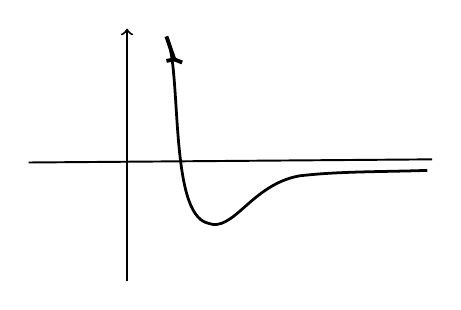
\begin{tikzpicture}[x=1.25cm, y=1cm]
\draw[->,line width=.7pt] (0,-1.5)--(0,1.7);
\draw[line width=.7pt] (-1,0)--(3.1,.04);
\draw[line width=1pt] (.4,1.6)..controls (.56,1.2) and (.42,-.65)..(.82,-.77)..controls (1.08,-.9) and (1.26,-.28)..(1.75,-.17)..controls (2.15,-.11) and (2.6,-.12)..(3.05,-.1);
\draw[line width=1.4pt] (.4,1.6)--(.48,1.31)--(.4,1.29);
\draw[line width=1.4pt] (.48,1.31)--(.56,1.27);
\end{tikzpicture}}}
\end{GelfandAdjacentEvidence}




\begin{GelfandAdjacentEvidence}{GELFAND-P000152}{3}
In the presence of $\delta$:
\SourceFigure{GELFAND-P000152}{hard-core-graph}{Two axes with arrows. At the right is a dotted vertical; above it $+\infty$, a thick mark at its intersection with the horizontal, and $\delta$ to the right. The branch leaves the thick mark for a well and rises below the horizontal axis. The dense ink at the intersection is rendered without an established function value at $\delta$ or an assertion of closedness.\par\smallskip\centering{\color{black}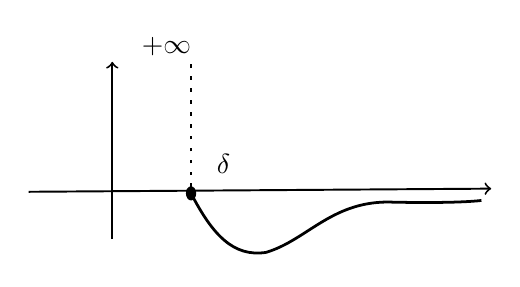
\begin{tikzpicture}[x=1.25cm, y=1cm]
\draw[->,line width=.7pt] (0,-.6)--(0,1.65);
\draw[->,line width=.7pt] (-.85,0)--(3.85,.04);
\draw[dash pattern=on 1.3pt off 3pt,line width=.8pt] (.8,.06)--(.8,1.65);
\node at (.55,1.85) {$+\infty$};
\node at (1.13,.35) {$\delta$};
\fill (.8,-.02) ellipse (.065cm and .09cm);
\draw[line width=1pt] (.8,-.02)..controls (1.02,-.55) and (1.23,-.83)..(1.56,-.77)..controls (1.97,-.62) and (2.22,-.13)..(2.8,-.13)..controls (3.12,-.14) and (3.55,-.14)..(3.75,-.11);
\end{tikzpicture}}}
\end{GelfandAdjacentEvidence}




\begin{GelfandAdjacentEvidence}{GELFAND-P000152}{4}
Sometimes only a potential of compact support is consid.
\Unclear{GELFAND-P000152}{potential-argument-glyph}{The repeated letter in $U (r)$ and the denominators has a loop-shaped top and a lower stroke to the right: $r$ / a $\tau$-like sign. Its rendering as $r$ is provisional; the original repetitions appear in the fragments.}
\end{GelfandAdjacentEvidence}




\begin{GelfandAdjacentEvidence}{GELFAND-P000153}{1}
\SourcePage{GELFAND-P000153}{unlabelled}
\uwave{The particles are small ($\delta\, [?]$) compared with the region.}
\Unclear{GELFAND-P000153}{top-smallness-glyph}{The sign in parentheses: $\delta$- / $r$-like; its upper part touches the upper frame boundary and is cut off.}
\end{GelfandAdjacentEvidence}


Consid. a seq. of vessels $\Omega_N$ which expands
and fills the whole space
(e.g. similar cubes)

\begin{GelfandAdjacentEvidence}{GELFAND-P000153}{2}
Let us consider
\begin{equation*}
\{\mathcal L_\sigma{}_{\Omega_N, N}\, [?], H^N_{m, U (r)}\}
\end{equation*}
\Unclear{GELFAND-P000153}{thermodynamic-state-glyph}{In the first brace a loop-shaped letter with a right loop: $\mathcal L_\sigma$ / a single $\mathcal G$-like sign; below are $\Omega_N, N$. The rendering of the principal sign is provisional.}
\end{GelfandAdjacentEvidence}

\begin{GelfandAdjacentEvidence}{GELFAND-P000153}{3}
\Unclear{GELFAND-P000153}{potential-argument-glyph}{The letter in $U (r)$ has a short loop-shaped top and a lower stroke to the right: $r$ / a $\tau$-like sign. Its rendering as $r$ is provisional; the original notation appears in the fragment.}
\end{GelfandAdjacentEvidence}

\begin{equation*}
\frac{|\Omega_N|}{N}\longrightarrow v\quad\text{(limiting specific volume)}
\end{equation*}
\begin{flushright}
$|\Omega_N|$ — the volume of the region $\Omega_N$
\end{flushright}
(Thermodyn. limiting transition)

In most cases everything depends only on $v$,
and the shape of the vessel is immaterial.


\par\noindent\begin{minipage}[t]{\linewidth}
\uwave{Gibbs distribution.}

\begin{GelfandAdjacentEvidence}{GELFAND-P000153}{4}
It is assumed that a probability distr. is given on $\mathcal L_\sigma\, [?]$
In the equilibrium case it is postulated
(if everything is independent of time)
\begin{equation*}
p (a)=\frac1Qe^{-\beta H (a)},\qquad\beta>0
\end{equation*}
\begin{equation*}
Q=\int_{\mathcal L_\sigma\, [?]}e^{-\beta H (a)}\, da.
\end{equation*}
\Unclear{GELFAND-P000153}{state-glyph}{The loop-shaped state-space letter: $\mathcal L_\sigma$ / a single $\mathcal G$-like sign; the right loop may be part of the letter or a separate $\sigma$. The form recurs beneath the integral.}
\end{GelfandAdjacentEvidence}
\end{minipage}\par



For lattice systems the same formula, but $p$ now gives
the probabilities themselves, rather than densities.

A phys. sys. with a given Gibbs distr. is called
a \uwave{small canonical ensemble}

\begin{GelfandAdjacentEvidence}{GELFAND-P000153}{5}
\begin{equation*}
\left (\begin{gathered}\text{in the classical case}\\
\mathcal L_\sigma{}_{\Omega, N}\, [?], H^N_{m, U (r),\beta}\end{gathered}\right)
\end{equation*}
\Unclear{GELFAND-P000153}{ensemble-state-glyph}{In the classical-case parenthesis the loop-shaped state-space sign recurs: $\mathcal L_\sigma$ / a single $\mathcal G$-like letter. Below are $\Omega, N$; $H$ has $N$ above and $m, U (r),\beta$ below.}
\end{GelfandAdjacentEvidence}


In the thermodyn. limiting transition identical
systems are always consid. ($\beta$ is also fixed)
\begin{equation*}
p (a)=\frac1Qe^{-\beta\frac1{2m}\sum p_i^2}e^{-\beta\sum U (|x_i-x_j|)}
\end{equation*}

\begin{GelfandAdjacentEvidence}{GELFAND-P000153}{6}
\begin{equation*}
\mathcal L_\sigma\, [?]=R^{\nu N}\times\Omega^N
\end{equation*}
\Unclear{GELFAND-P000153}{product-state-glyph}{The same loop-shaped state-space sign appears in the last line; its rendering as $\mathcal L_\sigma$ is provisional. At the right is $R^{\nu N}\times\Omega^N$.}
\end{GelfandAdjacentEvidence}



\begin{GelfandAdjacentEvidence}{GELFAND-P000154}{1}
\SourcePage{GELFAND-P000154}{16}
\hfill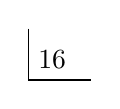
\begin{tikzpicture}[x=1cm, y=1cm, baseline=(pn.base)]
\node (pn) at (.3,.25) {$16$};
\draw[line width=.6pt] (0,.65)--(0,0)--(.8,0);
\end{tikzpicture}

Our distr. is a product of simpler distributions
and only the Gibbs distr. in the configuration space is of interest.
Where $U (r)\, [?]=+\infty$, the density will be $0$.
There are distr. fns. for a subsystem ($\int$ over the others)

\Unclear{GELFAND-P000154}{potential-argument-glyph}{The argument in $U (r)$: $r$ / a $\tau$-like handwritten sign with a short upper loop and a downward bend. Its rendering as $r$ is provisional.}
\end{GelfandAdjacentEvidence}


\uwave{Correlation functions} are convenient.
\begin{center}
\begin{tikzpicture}[x=1cm, y=1cm]
\node[anchor=north west, inner sep=0pt, text width=.58\linewidth, font=\small] (marginal) at (0,0) {
\begin{gather*}
p (x_1)=\frac1Q\int e^{-\beta\sum U (x_i-x_j)}\, dx_2\ldots dx_N\\
p (x_1,\ldots, x_k)=\ldots\int\ldots dx_{k+1}\ldots dx_N
\end{gather*}
};
\draw[line width=.6pt] ([xshift=-50mm,yshift=1mm]marginal.north west)--([xshift=-2mm,yshift=1mm]marginal.north west);
\draw[line width=.6pt] ([xshift=-2mm,yshift=1mm]marginal.north west)--([xshift=-2mm,yshift=-1mm]marginal.south west);
\draw[line width=.6pt] ([xshift=-3.5mm]marginal.north west)--([xshift=-3.5mm,yshift=-1mm]marginal.south west);
\draw[line width=.6pt] ([xshift=-3.5mm]marginal.south west)--(marginal.south east);
\end{tikzpicture}
\end{center}

\begin{GelfandAdjacentEvidence}{GELFAND-P000154}{2}

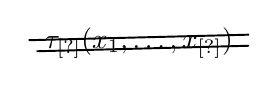
\begin{tikzpicture}[baseline=(cancelled.base)]
\node[inner sep=0pt] (cancelled) {$\tau_{[?]}(x_1,\ldots, x_{[?]})$};
\draw[line width=.7pt] ([xshift=-2mm,yshift=1pt]cancelled.west)--([xshift=2mm,yshift=3pt]cancelled.east);
\draw[line width=.7pt] ([xshift=-1mm,yshift=-3pt]cancelled.west)--([xshift=2mm,yshift=-1pt]cancelled.east);
\end{tikzpicture}
\Unclear{GELFAND-P000154}{cancelled-correlation}{A crossed-out expression resembling $\tau_k (x_1,\ldots, x_N)$ / $\tau_2(x_1,\ldots, x_2)$; the lower indices and middle strokes are covered by two lines. The original indices are not established.}
\end{GelfandAdjacentEvidence}
\begin{GelfandAdjacentEvidence}{GELFAND-P000154}{3}

\begin{equation*}
\tau_k (x_1,\ldots, x_k\mid N,\Omega,\beta)\, [?]=\frac{N!}{(N-k)!}p (x_1,\ldots, x_k)
\end{equation*}
\Unclear{GELFAND-P000154}{correlation-glyph}{The correlation sign has a short wave above and a downward bend: $\tau$ / an $r$-like sign. Here and in its repetitions $\tau$ is a provisional rendering.}
\end{GelfandAdjacentEvidence}


\uwave{Summatory fn.} $F (a)$, $a\,(x_1,\ldots, x_N)$

Of the 1st order $F (a)=f (x_1)+f (x_2)+\ldots+f (x_N)$

Of the 2nd order $F (a)=\sum_{i\ne j}f (x_i, x_j)$, $f$ — symmetric.

and so on.

\begin{GelfandAdjacentEvidence}{GELFAND-P000154}{4}

\uwave{Mean for summatory fns. $F$}:
\begin{align*}
\langle F\rangle&=N\langle f (x_1)\rangle=N\int_\Omega f (x)p (x)\, dx\\
&=\int_\Omega f (x)\tau_1(x)\, [?]\, dx
\end{align*}
(it suffices to know the 1st correlation function)
\Unclear{GELFAND-P000154}{first-moment}{In the first mean formula the sign before the index $1$ repeats the $\tau$ / $r$-like form; $\tau_1$ is a provisional rendering. Both integration regions are explicitly $\Omega$.}
\end{GelfandAdjacentEvidence}


\begin{GelfandAdjacentEvidence}{GELFAND-P000154}{5}
Similarly for the 2nd order:
\begin{equation*}
\langle F\rangle=\iint_{\Omega\,\Omega}f (x_1, x_2)\tau_2(x_1, x_2)\, [?]\, dx_1dx_2
\end{equation*}
\Unclear{GELFAND-P000154}{second-moment}{The second mean formula has the same $\tau$ / $r$-like sign, here with index $2$. Two $\Omega$ symbols are written beneath the double integral.}
\end{GelfandAdjacentEvidence}


\uwave{Probabilistic (phys.) meaning.}

$C\subset\Omega$, $C$ — a subregion, $n_C (a)$ — the number of particles
that fall in the subregion, $a=(x_1,\ldots, x_N)$.
This is a summatory quantity of the 1st order, with
\begin{equation*}
f (x)=\begin{cases}1,&x\in C,\\0,&x\notin C\end{cases}
\end{equation*}

\begin{GelfandAdjacentEvidence}{GELFAND-P000154}{6}
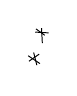
\begin{tikzpicture}[x=1mm, y=1mm, baseline=0pt]
\draw[line width=.35pt] (1,3.2)--(.9,5.1);
\draw[line width=.35pt] (.1,4.6)--(1.8,4.5);
\draw[line width=.35pt] (.2,5)--(1.3,4.2);
\draw[line width=.35pt] (-.8,1.6)--(.7,.6);
\draw[line width=.35pt] (-.7,.9)--(.6,1.8);
\draw[line width=.35pt] (-.1,2)--(.3,.4);
\end{tikzpicture}
\Unclear{GELFAND-P000154}{left-margin-marks}{Two small angular crossed signs in the left margin; their letter reading and meaning are not established.}
\end{GelfandAdjacentEvidence}


\begin{GelfandAdjacentEvidence}{GELFAND-P000154}{7}
Therefore
\begin{equation*}
\langle n_C (a)\rangle=\int_C\tau_1(x)\, [?]\, dx
\end{equation*}
\begin{equation*}
\frac{\langle n_C (a)\rangle}{|C|}=\frac1{|C|}\int\tau_1(x)\, [?]\, dx
\end{equation*}
\Unclear{GELFAND-P000154}{last-integral-domain}{No lower domain is visible on the final integral; the preceding formula explicitly has $C$. The repeated correlation sign is provisionally rendered as $\tau_1$.}
\end{GelfandAdjacentEvidence}



\begin{GelfandAdjacentEvidence}{GELFAND-P000155}{1}
\SourcePage{GELFAND-P000155}{unlabelled}
For a small region we obtain that
$\tau_1(x)\, [?]$ — the “local mean density”
at the point $x$.
\Unclear{GELFAND-P000155}{local-density-glyph}{At the beginning the sign before the index $1$: $\tau$ / an $r$-like handwritten sign; its rendering as $\tau_1$ is provisional.}
\end{GelfandAdjacentEvidence}


\begin{GelfandAdjacentEvidence}{GELFAND-P000155}{2}
\uwave{Another probabil. meaning}:
\SourceFigure{GELFAND-P000155}{small-neighbourhood}{A separate approximate circle with a dot inside; $\Delta C$ at the upper right edge and $x_0$ below.\par\smallskip\centering{\color{black}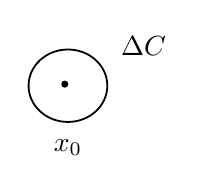
\begin{tikzpicture}[x=1cm, y=1cm]
\draw[line width=.65pt] (0,0) ellipse (.5cm and .46cm);
\fill (-.04,.02) circle (.045cm);
\node at (.96,.5) {$\Delta C$};
\node at (0,-.78) {$x_0$};
\end{tikzpicture}}}
\end{GelfandAdjacentEvidence}


$\Delta C$ — a small nbhd. of $x_0$.

\begin{GelfandAdjacentEvidence}{GELFAND-P000155}{3}
The probability that $n_{\Delta C}=1$
is $\tau_1(x_0)\, [?]\Delta C$.
\begin{equation*}
p (n_{\Delta C}=1)=\tau_1(x_0)\, [?]\Delta C+o (\Delta C)
\end{equation*}
\Unclear{GELFAND-P000155}{probability-expansion}{The provisionally rendered sign $\tau_1$ recurs in the verbal line and the equality. The last term is written $o (\Delta C)$.}
\end{GelfandAdjacentEvidence}
\begin{GelfandAdjacentEvidence}{GELFAND-P000155}{4}


\begin{tikzpicture}[x=1cm, y=1cm, baseline=0pt]
\fill (0,0)--(-.07,.05)--(-.08,.15)--(-.03,.12)--(.02,.15)--(.06,.13)--(.1,.18)--(.15,.16)--(.15,.07)--(.1,.03)--(.06,-.02)--cycle;
\end{tikzpicture}
\Unclear{GELFAND-P000155}{isolated-ink-mark}{Between the lines of the first probability explanation is a separate dense ink mark with an irregular outline; no letter reading or meaning is established.}
\end{GelfandAdjacentEvidence}


26/$\overline{\underline{\mathrm{IX}}}$. \uwave{Gelfand Sem}.

\uwave{R. A. Minlos}. \underline{Lecture 2}.

$\tau (x_1, x_2)\, [?]\Delta x_1\Delta x_2$ — the prob. of a
$\overset{\underbrace{\text{(one)}}}{\text{particle}}$ falling in $\Delta x_1$
and a second one in $\Delta x_2$.

\begin{GelfandAdjacentEvidence}{GELFAND-P000155}{5}
\Unclear{GELFAND-P000155}{two-particle-correlation-glyph}{Before $(x_1, x_2)$ is the same $\tau$ / $r$-like sign; no separate index $2$ is visible on it. Its rendering as $\tau$ is provisional.}
\end{GelfandAdjacentEvidence}

\begin{GelfandAdjacentEvidence}{GELFAND-P000155}{6}
\SourceFigure{GELFAND-P000155}{two-neighbourhoods}{Two separate approximate outlines, with $x_1, x_2$ below; dense crossed strokes inside, whose separate letter reading is not established. A short stroke above the right outline. Sizes and distance are not given.\par\smallskip\centering{\color{black}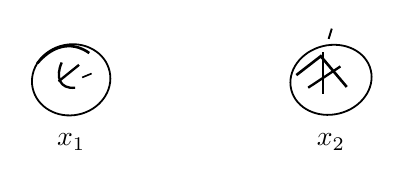
\begin{tikzpicture}[x=1cm, y=1cm]
\draw[line width=.65pt,rotate=12] (0,0) ellipse (.5cm and .45cm);
\draw[line width=.95pt] (-.43,.21)..controls (-.2,.48) and (.05,.47)..(.23,.34);
\draw[line width=.85pt] (-.12,.22)..controls (-.2,.04) and (-.15,-.12)..(.05,-.1);
\draw[line width=.85pt] (-.16,-.02)--(.1,.19);
\draw[line width=.6pt] (.14,.03)--(.26,.08);
\node at (0,-.79) {$x_1$};
\draw[line width=.65pt,rotate around={14:(3.3,0)}] (3.3,0) ellipse (.52cm and .44cm);
\draw[line width=.95pt] (2.86,.06)--(3.17,.3)--(3.5,-.09);
\draw[line width=.85pt] (3.2,.35)--(3.2,-.18);
\draw[line width=.85pt] (3.01,-.1)--(3.42,.17);
\draw[line width=.7pt] (3.27,.52)--(3.31,.65);
\node at (3.3,-.79) {$x_2$};
\end{tikzpicture}}}
\end{GelfandAdjacentEvidence}




$\Omega_N\longrightarrow\infty$ — the thermodyn. limiting transition.
\begin{equation*}
\frac{|\Omega_N|}{N}\longrightarrow v=\frac1\rho,\qquad\rho\text{ — density}.
\end{equation*}


\underline{Hypothesis}: 1)
\begin{equation*}
\tau_k (x_1,\ldots, x_k\mid N,\Omega,\beta)\, [?]\longrightarrow\vec\tau_k (x_1,\ldots, x_k\mid v,\beta)\, [?]
\end{equation*}
This is assumed (limiting correlation function)

\begin{GelfandAdjacentEvidence}{GELFAND-P000155}{7}
Moreover, it is assumed that $\forall\tau_k\ \exists v_N$ such that
\begin{equation*}
\bigl (v_N\ \underset{\longrightarrow}{\text{depends}}\text{ only on the vessel and on}\, [?]\ k\bigr)
\end{equation*}
\Unclear{GELFAND-P000155}{volume-parenthesis}{The short notation before $k$: “от” (on) / an “о.”-like contraction; the reading is not established. A separate right arrow beneath “depends.”}
\end{GelfandAdjacentEvidence}
\begin{GelfandAdjacentEvidence}{GELFAND-P000155}{8}

\begin{align*}
2)\quad &\left|\begin{aligned}
\tau_k (x_1,\ldots, x_k\mid N,\Omega,\beta)\, [?]\\[-.3ex]
-\vec\tau_k (x_1,\ldots, x_k\mid v_N,\beta)\, [?]
\end{aligned}\right|<\\
&<C_k\gamma\bigl (\min\underset{\text{dist.}}{|x_i,\partial\Omega|}\bigr),\\
&\text{where }\gamma (r)\longrightarrow0\text{ as }r\longrightarrow\infty.
\end{align*}
\Unclear{GELFAND-P000155}{correlation-glyph}{The principal letter: $\tau$ / an $r$-like sign. Above the limiting function is a horizontal stroke with a right-pointing head. In the bound $\gamma$ has a long lower stroke; “dist.” is written beneath $|x_i,\partial\Omega|$.}
\end{GelfandAdjacentEvidence}
\begin{GelfandAdjacentEvidence}{GELFAND-P000155}{9}

\begin{flushright}
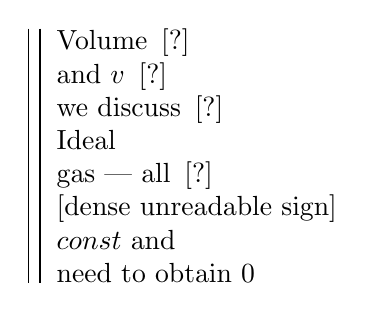
\begin{tikzpicture}[x=1cm, y=1cm]
\node[anchor=north west, inner sep=0pt, text width=.32\linewidth] (margin) at (0,0) {Volume\, [?]\par and $v$\, [?]\par we discuss\, [?]\par Ideal\par gas — all\, [?]\par [dense unreadable sign]\par $\operatorname{const}$ and\par need to obtain $0$};
\draw[line width=.65pt] ([xshift=-2mm]margin.north west)--([xshift=-2mm]margin.south west);
\draw[line width=.65pt] ([xshift=-3.5mm]margin.north west)--([xshift=-3.5mm]margin.south west);
\end{tikzpicture}
\end{flushright}
\Unclear{GELFAND-P000155}{right-margin}{Beyond two vertical lines are words resembling “Volume and $v$ we discuss,” then “Ideal gas — all” / “… without …,” $\operatorname{const}$, “and need to obtain $0$.” The first connective and endings are faint; a dense unreadable sign follows the gas line. These readings are provisional.}
\end{GelfandAdjacentEvidence}


\begin{GelfandAdjacentEvidence}{GELFAND-P000155}{10}
$\gamma$ depends on the potential.
For a potential of compact support $\gamma (r)\longrightarrow e^{-\lambda r}$.
\Unclear{GELFAND-P000155}{exponential-arrow}{A right arrow between $\gamma (r)$ and $e^{-\lambda r}$; separate limit conditions are not repeated in this line.}
\end{GelfandAdjacentEvidence}
\begin{GelfandAdjacentEvidence}{GELFAND-P000155}{11}

\sout{[unreadable sign]}
\Unclear{GELFAND-P000155}{cancelled-before-volume}{Before “We then have” a short sign or number is densely crossed out; the original reading is not established.}
\end{GelfandAdjacentEvidence}

We then have $v_N\longrightarrow v$ as $N\longrightarrow\infty$.

\begin{GelfandAdjacentEvidence}{GELFAND-P000155}{12}
3) Assume that the limiting correlation fns. are invariant under translations.
Hence $\vec\tau_1\, [?]=\operatorname{const}=\rho$.
\Unclear{GELFAND-P000155}{final-invariance-glyph}{In the last line the provisionally rendered sign $\tau_1$ recurs with a horizontal right arrow above it; then $\operatorname{const}=\rho$.}
\end{GelfandAdjacentEvidence}



\begin{GelfandAdjacentEvidence}{GELFAND-P000156}{1}
\SourcePage{GELFAND-P000156}{17}
\hfill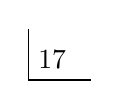
\begin{tikzpicture}[x=1cm, y=1cm, baseline=(pn.base)]
\node (pn) at (.3,.25) {$17$};
\draw[line width=.6pt] (0,.65)--(0,0)--(.8,0);
\end{tikzpicture}

4) Continuity with respect to $v$ and $\beta$.

This theorem should hold except at exceptional
values of $v$ and $\beta$. (assumed)

Proved only for small $v$ and $\beta$ (under some assumptions).
(this will be done later —
— Ruelle)


5) All $\vec\tau_k\, [?]$ are bounded.
\hfill
\begin{tikzpicture}[x=1cm, y=1cm, baseline=0pt]
\fill (0,.04)--(.16,.07)--(.16,-.05)--(.08,-.02)--(.02,-.04)--cycle;
\end{tikzpicture}
\Unclear{GELFAND-P000156}{limiting-correlation-glyph}{The principal letter is $\tau$- / $r$-like; its rendering as $\tau$ is provisional. Above it is a horizontal stroke with a right-pointing head; both lines of item $5$ have the index $k$.}
\end{GelfandAdjacentEvidence}
\begin{GelfandAdjacentEvidence}{GELFAND-P000156}{2}

$\vec\tau_k\, [?]$ exist for all $v$, not\, [?] for all $v$ with such\, [?]
a rate of convergence.
\Unclear{GELFAND-P000156}{fifth-hypothesis-correction}{The short word after the comma is “не” (not) / “но” (but). The beginning of the word rendered as “such” is densely overwritten; the original reading beneath the strokes is not established.}
\end{GelfandAdjacentEvidence}
\begin{GelfandAdjacentEvidence}{GELFAND-P000156}{3}

\begin{center}
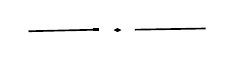
\begin{tikzpicture}[x=1cm, y=1cm]
\draw[line width=.6pt] (0,0)--(.87,.02);
\draw[line width=1.2pt] (.82,.02)--(.9,.02);
\fill (1.08,.015)--(1.13,.04)--(1.18,.015)--(1.13,-.01)--cycle;
\draw[line width=.6pt] (1.35,.02)--(2.25,.035);
\end{tikzpicture}
\end{center}
\Unclear{GELFAND-P000156}{separators-and-ink}{At the right beside item $5$ is a separate small dense mark with an irregular outline; no letter reading is established. Below are two horizontal rules and a separate diamond-shaped central dot; the right end of the left rule is thickened.}
\end{GelfandAdjacentEvidence}


\begin{GelfandAdjacentEvidence}{GELFAND-P000156}{4}
\uwave{On the Gibbs distribution.} (at Gelfand's request)
\begin{equation*}
a (p_1,\ldots, p_N, x_1,\ldots, x_N)
\end{equation*}
\SourceFigure{GELFAND-P000156}{energy-circle}{One unfilled approximate circle without labels or arrows to the left of the paragraph on motion; no sizes are specified.\par\smallskip\centering{\color{black}\begin{tikzpicture}[x=1cm, y=1cm]
\draw[line width=.65pt,rotate=-4] (0,0) ellipse (.62cm and .55cm);
\end{tikzpicture}}}
\end{GelfandAdjacentEvidence}



Motion on the surface of constant energy $H (a)=\operatorname{const}$.
Assume that it is ergodic and there is an invariant measure.

Perhaps any distribution, as the number of particles increases,
leads to the Gibbs distribution. (Gelfand)

Not any: if there is no ergodic hypothesis (Arnold)
\begin{center}
\begin{tikzpicture}[x=1cm, y=1cm]
\draw[line width=.6pt] (0,0)--(.9,.04);
\draw[line width=1.15pt] (.83,.035)--(.91,.04);
\fill (1.09,.02) circle (.035cm);
\draw[line width=.6pt] (1.3,.025)--(2.28,.09);
\end{tikzpicture}
\end{center}


\uwave{Representativity of mean values.}
\begin{equation*}
P_\sigma\, [?]\bigl (|F-\langle F\rangle|>\varepsilon\bigr)\longrightarrow0
\quad\text{as the number of particles increases.}
\end{equation*}
Then the random variable (function; physical quantity) is called
representative.

\begin{GelfandAdjacentEvidence}{GELFAND-P000156}{5}
This is imprecise, since there is no single function $F$.
\Unclear{GELFAND-P000156}{probability-subscript}{The subscript of $P$ is short, with an upper hook and a lower loop: $\sigma$ / $\tau$ / an $r$-like sign. Its rendering as $\sigma$ is provisional. The heading has a wavy underline; below it is the remark about the absence of a single function $F$.}
\end{GelfandAdjacentEvidence}


\uwave{The needed example.} (summatory function)
\begin{equation*}
F_N (x_1,\ldots, x_N)=\sum_{i\ne j}f (x_i-x_j),
\end{equation*}
$f$ is one and the same, $\displaystyle\int|f (\xi)|\, d\xi<\infty$.

\begin{GelfandAdjacentEvidence}{GELFAND-P000156}{6}
\begin{align*}
\langle F_N\rangle
&=\iint\tau_2\, [?](x_1, x_2\mid N,\Omega,\beta)f (x_1-x_2)\, dx_1\, dx_2=\\
&=\iint\vec\tau_2\, [?](x_1-x_2\mid v,\beta)f (x_1-x_2)\, dx_1\, dx_2+o (|\Omega|)=\\
&=|\Omega|\int\vec\tau_2\, [?](\xi\mid v,\beta)f (\xi)\, d\xi+o (|\Omega|).
\end{align*}
\Unclear{GELFAND-P000156}{mean-correlation-glyph}{In the first line the principal $\tau$- / $r$-like sign has no stroke above it; in the following two it has a stroke with a right-pointing head. All three lines have the index $2$. The letter is rendered provisionally. Integration domains are not separately indicated; equality signs are repeated at the ends and beginnings of the lines.}
\end{GelfandAdjacentEvidence}
\begin{GelfandAdjacentEvidence}{GELFAND-P000156}{7}

\begin{flushright}
\begin{tikzpicture}[x=1cm, y=1cm, baseline=0pt]
\draw[line width=.7pt] (0,.02)..controls (-.18,.1) and (-.05,.25)..(.1,.18)..controls (.22,.12) and (.06,-.09)..(-.09,-.04);
\draw[line width=.55pt] (-.14,-.06)--(.58,.22);
\draw[line width=.55pt] (-.1,-.1)--(.62,.18);
\node at (1,.27) {$+$};
\node at (2.55,.27) {$F\, [?]$};
\draw[line width=.6pt] (1.55,-.08)--(2.91,.63);
\draw[line width=.6pt] (1.6,-.16)--(2.98,.57);
\draw[line width=.45pt] (1.62,-.22)--(2.85,.48);
\end{tikzpicture}
\end{flushright}
\Unclear{GELFAND-P000156}{cancelled-final-equation}{To the right of the last equality, a loop-shaped sign, a plus and an $F$-like form are crossed out. The first reading is not established; $F$ is provisional. The cancellation strokes are diagonal.}
\end{GelfandAdjacentEvidence}


\begin{GelfandAdjacentEvidence}{GELFAND-P000156}{8}
Thus,
\begin{equation*}
\left\langle\frac{F_N}{N}\right\rangle\sim v\int\vec\tau_k\, [?](\xi\mid v,\beta)f (\xi)\, d\xi
\quad\text{— already }\operatorname{const}.
\end{equation*}
\Unclear{GELFAND-P000156}{final-index}{The final index is $k$- / $2$-like; its rendering as $k$ is provisional. Above the principal letter is a horizontal stroke with a right-pointing head; the letter itself is $\tau$- / $r$-like. Before the integral, $v$ is written.}
\end{GelfandAdjacentEvidence}



\begin{GelfandAdjacentEvidence}{GELFAND-P000157}{1}
\SourcePage{GELFAND-P000157}{unlabelled}
\begin{tikzpicture}[x=1cm, y=1cm, baseline=(cancel.base)]
\node (cancel) at (0,0) {$6\, [?]$};
\draw[line width=1.15pt] (-.22,-.02)--(.22,.06);
\draw[line width=.9pt] (-.2,.04)--(.2,.12);
\fill (.35,.02) circle (.035cm);
\end{tikzpicture}
\Unclear{GELFAND-P000157}{cancelled-top-number}{In the upper left margin is a densely cancelled loop-shaped sign resembling $6$; its original reading is not established. At its right is a separate dot.}
\end{GelfandAdjacentEvidence}
\begin{GelfandAdjacentEvidence}{GELFAND-P000157}{2}

One more hypothesis (but it already follows from these,
though with difficulty):
\begin{align*}
6)\quad&\left|\begin{aligned}
\bar\tau_{k+s}(x_1,\ldots, x_k, y_1,\ldots, y_s\mid v,\beta)\\[-.3ex]
-\bar\tau_k (x_1,\ldots, x_k\mid v,\beta)\bar\tau_s (y_1,\ldots, y_s\mid v,\beta)
\end{aligned}\right|\, [?]\le\\
&\le C_{k, s}\gamma\bigl (\min_{i, j}|x_i-y_j|\bigr)\, [?].
\end{align*}
(multiplicative property; for the ideal gas $0$).
\Unclear{GELFAND-P000157}{hypothesis-correlation-glyph}{The principal letter in all three functions is $\tau$- / $r$-like; its rendering as $\tau$ is provisional. Above each is a flat horizontal stroke. The minimum has $i, j$; between $x_i$ and $y_j$ is a dense horizontal sign rendered as a minus. The $\le$ signs are repeated at the end and beginning of the lines.}
\end{GelfandAdjacentEvidence}


We shall prove that
\begin{equation*}
\underset{\text{variance}}{DF_N}\sim dN,\qquad d\text{ — }\operatorname{const}.
\end{equation*}
Hence $D\frac{F_N}{N}\sim\frac dN$ and by Chebyshev's inequality we already

\begin{GelfandAdjacentEvidence}{GELFAND-P000157}{3}
obtain
\begin{tikzpicture}[x=1cm, y=1cm, baseline=(word.base)]
\node[inner sep=1pt] (word) at (0,0) {[unreadable word]};
\draw[line width=.9pt] (word.west)--(word.east);
\draw[line width=.8pt] ([yshift=-1mm]word.west)--([yshift=1mm]word.east);
\draw[line width=.6pt] (-.65,-.05)..controls (-.95,-.5) and (-.65,-.5)..(-.48,-.18);
\end{tikzpicture}
representativity of the mean.
\Unclear{GELFAND-P000157}{cancelled-representative-word}{After “obtain” a word is densely cancelled, with a loop-shaped stroke below it. Its original reading, including a possible repetition of “represent.”, is not established. The following words are “representativity of the mean”.}
\end{GelfandAdjacentEvidence}

This is proved by direct calculation:
\begin{equation*}
DF_N=\langle F_N^2\rangle-\langle F_N\rangle^2.
\end{equation*}

\begin{GelfandAdjacentEvidence}{GELFAND-P000157}{4}
\begin{align*}
\begin{tikzpicture}[x=1cm, y=1cm, baseline=(square.base)]
\node (square) at (0,0) {$F_N^2$};
\node[anchor=north east, align=left, inner sep=1pt] (ann) at (.25,-.56) {$\substack{\text{summatory}\, [?]\\\text{qty. of 4th ord.}}$};
\draw[line width=.65pt] (-.42,-.18)..controls (-.28,-.45) and (.28,-.45)..(.42,-.18);
\draw[line width=.55pt] ([xshift=-1mm,yshift=-2mm]ann.south west)..controls ([yshift=-2mm]ann.south) and ([xshift=3mm,yshift=-2mm]ann.south east)..([xshift=4mm,yshift=-1mm]ann.south east)..controls ([xshift=6mm]ann.east) and ([xshift=5mm,yshift=-1mm]ann.north east)..([xshift=3mm,yshift=-1mm]ann.north east);
\end{tikzpicture}
&=2\sum_{i\ne j}f^2(x_i-x_j)\\
&\quad+4\sum_{\substack{i, j, k\, [?]\\\text{noncoinc.}\, [?]}}f (x_i-x_j)f (x_k-x_j)+\\
&\quad+\sum_{\substack{i, j, k, s\\\text{unequal}}}f (x_i-x_j)f (x_k-x_s).
\end{align*}
\Unclear{GELFAND-P000157}{sum-labels}{Beneath $F_N^2$ is a short arc; at the left is “summatory” or a similar abbreviation, then “qty. of 4th ord.”, enclosed below by a long curved rule. Beneath the triple sum are $i, j$ and a dense $k$-like third sign and an abbreviation resembling “noncoinc.”; these readings are provisional. Beneath the quadruple sum are $i, j, k, s$ and “unequal”.}
\end{GelfandAdjacentEvidence}


\begin{GelfandAdjacentEvidence}{GELFAND-P000157}{5}

We calculate
\begin{equation*}
\langle F_N^2\rangle=2\iint f^2(x_1-x_2)\tau_2\, [?](x_1, x_2)\, dx_1\, dx_2+4\ldots
\end{equation*}
and use the decay estimates.
\Unclear{GELFAND-P000157}{terminal-correlation-glyph}{The function in the last integral has a principal $\tau$- / $r$-like sign without a stroke above it and the index $2$; its rendering as $\tau$ is provisional. It is followed by $+4\ldots$ and the complete line about decay estimates.}
\end{GelfandAdjacentEvidence}



\begin{GelfandAdjacentEvidence}{GELFAND-P000158}{1}
\SourcePage{GELFAND-P000158}{18}
\hfill\begin{tikzpicture}[x=1cm, y=1cm, baseline=(pn.base)]
\node (pn) at (.3,.25) {$18$};
\draw[line width=.6pt] (0,.65)--(0,0)--(.8,0);
\end{tikzpicture}

\underline{D. Kazhdan.} \uwave{His results.}

1) $G$ is a simple real or $p$-adic Lie group containing
as a subgroup $SL (3, P)\, [?]$, $P\, [?]$ is the corresponding field.
$\Gamma$ is a discrete subgroup with a quotient space of finite volume.
\Unclear{GELFAND-P000158}{field-and-group-glyphs}{In the argument of $SL (3, P)$ and before “corresponding field” is a sign with an upper loop and a descending stroke: $P$ / a $\rho$-like form. Its rendering as $P$ is provisional.}
\end{GelfandAdjacentEvidence}

Then a)
\begin{equation*}
\Gamma/\underset{\substack{\vert\\\text{commutator subgroup}}}{[\Gamma,\Gamma]}\quad\text{is finite}.
\end{equation*}
b) $\Gamma$ has a finite number of generators.
(even from any set of generators a finite one can be selected)


2) $G$ is an algebraic group over the rational numbers $Q$, containing
$SL (3, Q)$.
Something about representations.

The \uwave{proof} uses the isolation of the trivial representation.

\begin{GelfandAdjacentEvidence}{GELFAND-P000158}{2}

\underline{\uwave{Prof. Lodzhs.\, [?] (Canada)}} jointly with \uwave{P. Szego}.
\Unclear{GELFAND-P000158}{lecturer-name}{The name: “Лоджс.” / “Ходжс.” / “Лорчс.” / “Лорче.”; the first letter is dense, the middle has a conspicuous upper loop, and the ending is $c$-like. The reading is provisional. Beneath the professor/Canada line are wavy and straight rules; beneath P. Szego is a wavy rule.}
\end{GelfandAdjacentEvidence}
\begin{GelfandAdjacentEvidence}{GELFAND-P000158}{3}

\begin{equation*}
y''+f (x)y=0,\qquad0<x<\infty.
\end{equation*}
\SourceFigure{GELFAND-P000158}{oscillating-solution}{A horizontal line, a short vertical at the left, four dense early crossings and a dot at the bottom of the vertical. Three upper waves alternate with lower ones, ending at the right in a short downward curl. No labels, sizes or exact coordinates are given; the contour is approximate.\par\smallskip\centering{\color{black}\begin{tikzpicture}[x=1cm, y=1cm]
\draw[line width=.65pt] (-.85,-.02)--(4.35,.02);
\draw[line width=.65pt] (0,.72)--(0,-.58);
\draw[line width=.85pt] (0,0)..controls (.13,.6) and (.5,.65)..(.82,.62)..controls (1.02,.61) and (1.08,.27)..(1.18,0)..controls (1.32,-.58) and (1.73,-.7)..(2.04,0)..controls (2.2,.4) and (2.48,.58)..(2.65,0)..controls (2.78,-.44) and (3.01,-.48)..(3.13,0)..controls (3.25,.31) and (3.5,.43)..(3.47,0)..controls (3.53,-.18) and (3.65,-.17)..(3.74,-.13);
\fill (0,0) circle (.065cm);
\fill (1.18,0) circle (.065cm);
\fill (2.04,0) circle (.065cm);
\fill (2.65,0) circle (.065cm);
\fill (0,-.58) circle (.035cm);
\end{tikzpicture}}}
\end{GelfandAdjacentEvidence}




\uwave{Sturm:} (1836)
if $f (x)$ increases, the zeros get closer
and conversely.

\par\noindent\begin{minipage}[t]{\linewidth}
\uwave{Theorem,} if $f$ has a higher degree of monotonicity.

Let
\begin{equation*}
(-1)^j f^{(j+1)}(x)\ge0,\qquad0<x<\infty,\quad j=1,\ldots, N
\end{equation*}
\end{minipage}\par
and $f (\infty)>0$. Then
\begin{equation*}
(-1)^n\Delta^{n+1}x_k>0,\qquad n=1,\ldots, N+1;\quad k=1,2,\ldots
\end{equation*}

\begin{GelfandAdjacentEvidence}{GELFAND-P000158}{4}
This holds for the Bessel functions
\raisebox{.65ex}{\begin{tikzpicture}[baseline=(order.base)]
\node[draw, ellipse, inner sep=2pt, line width=.6pt] (order) {$\nu>\frac12\, [?]$};
\end{tikzpicture}}, \textbf{A}iry\, [?] and others.
\Unclear{GELFAND-P000158}{bessel-insertion}{In an oval above the line after Bessel: $\nu>1/2$ / $v>1/2$; the sign and dense fraction are rendered provisionally. The next name is Airy / Аiry: the initial $A$-like sign is densely overwritten, then a dot above $i$, an $r$-like bridge and a lower $y$-loop.}
\end{GelfandAdjacentEvidence}


The wave areas have the same property.
\begin{equation*}
M_k=\int_{x_k}^{x_{k+1}}|y (x)|^\lambda\, dx,\qquad\lambda>-1.
\end{equation*}
$\lambda=0$ — differences of zeros, $\lambda=1$ — wave areas,

\begin{GelfandAdjacentEvidence}{GELFAND-P000158}{5}
$\lambda=-1$ —
$\underset{\text{([unreadable abbreviation] parts)}}{\text{diff. of derivs.}}$
(Gelfand's remark) $\dfrac1{y'(x_k)}$.
\Unclear{GELFAND-P000158}{last-parenthesis}{Beneath “diff. of derivs.” is a parenthesis: “ин. части” / “м. части” / “… parts”; the first abbreviation is not established. The main line has $\lambda=-1$; at the right is $1/y'(x_k)$.}
\end{GelfandAdjacentEvidence}



\begin{GelfandAdjacentEvidence}{GELFAND-P000159}{1}
\SourcePage{GELFAND-P000159}{unlabelled}
\underline{\underline{I. M. Gelfand.}}

Repetition of I. Bernstein. (also Atiya)

$G$ is a compact group.
$K_G$ is a functor, $K_G (X)$.

\SourceFigure{GELFAND-P000159}{bundle-map}{$E$ above $X$, with a downward arrow between them and no additional labels.\par\smallskip\centering{\color{black}\begin{tikzpicture}[x=1cm, y=1cm]
\node at (0,.7) {$E$};
\draw[->,line width=.7pt] (0,.4)--(0,-.4);
\node at (0,-.7) {$X$};
\end{tikzpicture}}}
\end{GelfandAdjacentEvidence}



$E, X$ are $G$-spaces; a vector bundle.
Fiber to fiber — linearly.
Formal differences.

This is a contravariant functor.


\uwave{Generalization of the notion of a classifying space.}
Consider
\begin{equation*}
E\times_G X=X_G.
\end{equation*}
the orbits of $G$ are contracted to a point; $E$ is the universal space.

\begin{GelfandAdjacentEvidence}{GELFAND-P000159}{2}
If $\boldsymbol X$ is a point, then $X_G=B_G$, i.e. $*_G=B_G$.
\Unclear{GELFAND-P000159}{cancelled-point-x}{After “If” a dense $X$ is written over earlier strokes. Their original reading is not established.}
\end{GelfandAdjacentEvidence}


\underline{Theorem.} $K_G (X)$ approximately coincides with $K (X_G)$
(already the ordinary $K$-functor)

$K_G (X)$ is a ring, $X\longrightarrow\bullet$, hence $R_G\longrightarrow K_G (X)$

\begin{GelfandAdjacentEvidence}{GELFAND-P000159}{3}
and therefore
\begin{tikzpicture}[x=1cm, y=1cm, baseline=(word.base)]
\node[inner sep=1pt] (word) at (0,0) {[unreadable word]};
\draw[line width=.85pt] (word.west)--(word.east);
\draw[line width=.7pt] ([yshift=-1mm]word.west)--([yshift=2mm]word.east);
\draw[line width=.6pt] ([yshift=1mm]word.west)--([yshift=3mm]word.east);
\draw[line width=.55pt] (-.8,.1)..controls (-1.1,-.5) and (-.85,-.45)..(-.55,-.2);
\end{tikzpicture}
this is an $R_G$-module (a ring over a subring)
\Unclear{GELFAND-P000159}{cancelled-module-word}{Between “therefore” and “this” a word or group of letters is densely cancelled, with a loop-shaped stroke below it; the original reading is not established.}
\end{GelfandAdjacentEvidence}


\underline{I. Bernstein.} The most essential part of the proof: a construction with
elliptic operators.

\begin{GelfandAdjacentEvidence}{GELFAND-P000159}{4}
\SourceFigure{GELFAND-P000159}{fibration-map}{$Y$ above $X$, a downward arrow, and $M_x$ to its right. Beside it is the description of $M$ as the fiber and the arrow $K (X)\longrightarrow K (Y)$.\par\smallskip\centering{\color{black}\begin{tikzpicture}[x=1cm, y=1cm]
\node at (0,.7) {$Y$};
\draw[->,line width=.7pt] (0,.4)--(0,-.4);
\node at (0,-.7) {$X$};
\node at (.65,-.05) {$M_x$};
\end{tikzpicture}}}
\end{GelfandAdjacentEvidence}


$M$ is a manifold, the fiber; $K (X)\longrightarrow K (Y)$.
Sometimes a reverse map can be constructed.

Let there be on $X$ a family of differential operators $D_x$:
acting in a sheaf over $M_x$ (the fibers over $x$).
Let there be over $Y$ $2$ sheaves $N_1, N_2$.
\begin{equation*}
D_x:\Gamma (N_1|_{M_x})\longrightarrow\Gamma (N_2|_{M_x})
\end{equation*}
— an elliptic operator (or a complex)

For example, the de Rham complex.

$K (Y)$ is a $K (X)$-module. Construct such a map of $K (X)$-modules.
$V$ is a sheaf on $Y$.
\begin{equation*}
M_x:\quad D_x\otimes1:\Gamma (N_1\otimes V)_{M_x}\longrightarrow\Gamma (N_2\otimes V)_{M_x}.
\end{equation*}

An elliptic operator; $\operatorname{Ker},\operatorname{Coker}<\infty$.
The difference of elements in the $K$-functor gives the required element.



\clearpage

\begin{GelfandAdjacentEvidence}{GELFAND-P000160}{1}
\SourcePage{GELFAND-P000160}{19}
\hfill\begin{tikzpicture}[x=1cm, y=1cm, baseline=(pn.base)]
\node (pn) at (.3,.25) {$19$};
\draw[line width=.6pt] (0,.65)--(0,0)--(.8,0);
\end{tikzpicture}


If there is a map
\begin{equation*}
X\longrightarrow\underset{\text{Fredholm ops.}}{F (H, H\, [?])}
\end{equation*}
\Unclear{GELFAND-P000160}{second-h}{The second letter inside $F (H, H)$ is densely overwritten; an $H$-like sign with lower strokes. The original form beneath them is not established.}
\end{GelfandAdjacentEvidence}
\begin{GelfandAdjacentEvidence}{GELFAND-P000160}{2}

then one can def. $\mathrm{Ker}-\mathrm{Coker}$ as a bundle over $X$
\begin{gather*}
x\longrightarrow A_x\\
x\longrightarrow A_x (1-t)+t\cdot A_xP_v
\end{gather*}
\begin{flushright}
$P_v$ — a projector. onto a дп.\, [?] subspace\\
to $V$.
\end{flushright}
\Unclear{GELFAND-P000160}{projector-subscript}{The small subscript of $P$ in the formula and explanation is $v$- / $V$-like; below it the subspace is denoted by capital $V$.}
\end{GelfandAdjacentEvidence}

\begin{GelfandAdjacentEvidence}{GELFAND-P000160}{3}
\Unclear{GELFAND-P000160}{projector-definition-abbreviation}{Before “subspace” is an abbreviation resembling “дп.” / “дн.”; the second letter has a joined lower stroke. It is provisionally rendered as “дп.” without expansion. Beneath the end of the line, “к $V$” (“to $V$”) is written separately.}
\end{GelfandAdjacentEvidence}


Already const. dim. of the kernel (locally)

Bundle \uwave{$ind\ V$}.


Next time, Nirenberg's report and Minlos.



\begin{GelfandAdjacentEvidence}{GELFAND-P000161}{1}
\SourcePage{GELFAND-P000161}{unlabelled}
$3/\overline{\underline{\mathrm{X}}}$.\quad \uwave{Gelfand's sem.}

\uwave{Nirenberg.}


Informal expos. of \uwave{Seeley and H\"ormander's index f-la.}
The f-la is analytic, without any topology, no connections with topology and how the leading terms disappear in it.
However, according to Gelfand, the Atiyah--Singer f-la can be written analyt. [as the degree of a mapping, etc.]
The same situation for Pontryagin classes.


$L$ --- ellipt. operator on a comp. m-fold. Consid.\, [?] eigenfns.
\Unclear{GELFAND-P000161}{eigenfunction-description}{Before ``eigenfns.'', the abbreviation is ``Рассм.'' / ``Расм.'': the middle joined strokes are not completely separable. Provisionally rendered as ``Consid.'', without expansion.}
\end{GelfandAdjacentEvidence}
\begin{GelfandAdjacentEvidence}{GELFAND-P000161}{2}

\begin{gather*}
L^*L\Psi=\lambda\Psi,\qquad \lambda>0,\\
LL^*(L\Psi)=\lambda L\Psi.
\end{gather*}
\begin{center}
\begin{tikzpicture}[x=1cm, y=1cm]
\draw[dashed,line width=.45pt] (0,0)--(6.2,0);
\end{tikzpicture}
\end{center}
\begin{equation*}
\Big\Vert\qquad \text{\uwave{$LL^*\varphi=\lambda\varphi\ \Rightarrow\ \varphi=L\Psi$}}
\end{equation*}
\SourceFigure{GELFAND-P000161}{positive-eigenspaces}{Below the second formula is a dashed line. The formula on the right is separated by a double vertical line and has a wavy underline.}
\end{GelfandAdjacentEvidence}
\begin{GelfandAdjacentEvidence}{GELFAND-P000161}{3}

\begin{equation*}
E_\lambda (L^*L)\overset{L\, [?]}{\longleftrightarrow}E_\lambda (LL^*),\qquad
\text{their }\mathrm{dim}=d_\lambda\quad
\substack{\text{for }\lambda>0!\\(\text{but not for }\lambda=0)}
\end{equation*}
\Unclear{GELFAND-P000161}{eigen-arrow-label}{Above the two-way arrow is a small sign with a vertical stroke and a lower stroke to the right, resembling $L$ / $l$; the upper dot meets the level of the dashed line. Provisionally rendered as $L$.}
\end{GelfandAdjacentEvidence}


One can consider
\begin{equation*}
(I+L^*L)^s,\qquad \mathrm{Re}\, s\ll0
\end{equation*}

\begin{GelfandAdjacentEvidence}{GELFAND-P000161}{4}

Then this is an integr. operator with a good kernel and its action is expressed through eigenfns.
[Crossed out: unread word.]
\Unclear{GELFAND-P000161}{cancelled-action-word}{Below ``eigenfns.'' a word resembling ``original'' is densely crossed out; the internal joined strokes do not permit a confident complete reading.}
\end{GelfandAdjacentEvidence}

\begin{gather*}
\int K_s (x, y)u (y)\, dy=\\
=\int\sum_j\Psi_j (x)\overline{\Psi}_j (y)(1+\lambda_j)^s u (y)\, dy
\end{gather*}

$\Psi_j$ --- scalar fns. or sections of a bundle.

\begin{GelfandAdjacentEvidence}{GELFAND-P000161}{5}

\begin{gather*}
\mathrm{Tr}\,(I+L^*L)^s=\int\mathrm{Tr}\, K_s (x, x)\, dx\\
=\int\sum\Psi_j (x)\overline{\Psi}_j (x\, [?])(1+\lambda_j\, [?])^s\, dx=\\
=\sum d_{\lambda_j}(1+\lambda_j)^s
\end{gather*}
\Unclear{GELFAND-P000161}{trace-faded-argument}{In the second integral the argument after $\overline{\Psi_j}$ and the beginning of the parenthesis $(1+\lambda_j)$ are very faint: $x$ / another faint argument; $1+$ / faint strokes.}
\end{GelfandAdjacentEvidence}



Consider
\begin{equation*}
\mathrm{Tr}\,(I+L^*L)^s-\mathrm{Tr}\,(I+LL^*)^s=
\end{equation*}
Everything cancels, except the terms with $\lambda=0$

\begin{GelfandAdjacentEvidence}{GELFAND-P000161}{6}
\begin{equation*}
=\mathrm{dim}\,\mathrm{ker}\, L-\mathrm{dim}\,\mathrm{ker}\, L^*=\text{\ae}\, [?](L)\qquad\text{--- index!}
\end{equation*}
\Unclear{GELFAND-P000161}{index-glyph}{The sign before $(L)$ has two joined loops: $\chi$ / $x$ / an ``æ''-like sign. Provisionally rendered as ``æ''.}
\end{GelfandAdjacentEvidence}


$(L^*L\varphi=0\ \Rightarrow\ L\varphi=0\ \text{etc.})$

Does not depend on $s$!


What follows --- study of the trace of integr. operators.



\begin{GelfandAdjacentEvidence}{GELFAND-P000162}{1}
\SourcePage{GELFAND-P000162}{25}
\hfill\begin{tikzpicture}[x=1cm, y=1cm, baseline=(pn.base)]
\node (pn) at (.4,.3) {$25$};
\draw[line width=.55pt] (.9,.72)--(0,.72)--(0,0)--(.9,0);
\end{tikzpicture}


$A$ --- $\underset{\text{of order }m>0.}{\text{ellipt.}}$ --- $(I+L^*L)$ ---
\begin{equation*}
|\arg a (x,\xi)-\pi|\geq\delta>0,\qquad |\xi|=1
\end{equation*}
\begin{center}
$\vert$\\[-.3ex]
this is assumed
\end{center}
(a more gen. situation than $I+L^*L$)
\begin{equation*}
\sigma (A)=a_m (x,\xi)+a_{m-1}(x,\xi)+\ldots
\end{equation*}
\SourceFigure{GELFAND-P000162}{elliptic-assumption}{Below ``ellipt.'': ``of order $m>0$.''. Below the angular condition: a short vertical stroke and ``this is assumed''.}
\end{GelfandAdjacentEvidence}


Take $m=1$ (multipl. by an invertible one)

\begin{GelfandAdjacentEvidence}{GELFAND-P000162}{2}
usual def.:
\begin{gather*}
A^s=\frac{1}{2\pi i}\int\lambda^s (\lambda-A)^{-1}\, d\lambda,\qquad
\|(\lambda-A)^{-1}\|\leq\frac{C}{1+|\lambda|}
\end{gather*}
\begin{center}
\begin{tikzpicture}[x=1cm, y=1cm]
\draw[line width=.65pt] (0,.25)--(4.25,.25)..controls (4.8,.25) and (4.8,-.25)..(4.25,-.25)--(0,-.25);
\draw[dashed,line width=.55pt] (0,0)--(3.05,0);
\draw[->,line width=.65pt] (3.05,0)--(4.3,.08);
\draw[line width=1.15pt] (4.38,-.20)..controls (4.68,-.40) and (4.38,-.47)..(4.32,-.34)..controls (4.32,-.26) and (4.48,-.23)..(4.48,-.25);
\node[anchor=west] at (5,0) {contour, enclos. spectrum.};
\end{tikzpicture}
\end{center}
\Unclear{GELFAND-P000162}{contour-direction}{Two long lines, open on the left, joined by a rounded turn on the right; inside, a dashed line with an arrow to the right. Thickening at the bottom of the right turn: the direction of traversal is undetermined.}
\end{GelfandAdjacentEvidence}


Thus for negat. powers. For posit. powers multiply by a positive integer power.


We must compute $\int\mathrm{Tr}\, K_s (x, x)\, dx$

$K_s (x, x)$ --- kernel of the operator $A^s$, $\mathrm{Re}\, s\ll0$.


(i) $s\longrightarrow K_s$ --- holom. mapping of the region $\mathrm{Re}(ms)<-n-k$ into kernels of class $C^k$ on $M\times M$

(smooth dep. of the kernel on $s$)

\begin{GelfandAdjacentEvidence}{GELFAND-P000162}{3}

(ii) $C$ --- comp. in $M\times M$, not [Crossed out: unread word.] [Inserted above with a bracket: intersec. with] the diagonal, then
\Unclear{GELFAND-P000162}{cancelled-intersection}{Between ``not'' and ``the diagonal'' a word is densely crossed out; above it, ``intersec. with'' is inserted with a bracket. Beneath the cancellation are separate loops without a confident literal reading.}
\end{GelfandAdjacentEvidence}
\begin{GelfandAdjacentEvidence}{GELFAND-P000162}{4}

$s\longrightarrow K_s|_C$ continues [Crossed out: unread short word.] to a holom. mapping
\Unclear{GELFAND-P000162}{cancelled-continuation}{After ``continues'' a short word resembling ``all'' / ``everything'' is crossed out.}
\end{GelfandAdjacentEvidence}

of the entire plane into $C^\infty (C)$

(not analyt. in $x$, since the coeffs. are infinitely differ.)


(iii) for every $x$, $K_s (x, x)$ is a meromorphic fn. on the entire plane with poles (simple), possibly only at
\begin{gather*}
-\frac{n}{m},\quad\frac{1-n}{m},\quad\frac{2-n}{m},\ldots,
-\frac{1}{m},\quad\frac{1}{m},\quad\frac{2}{m},\ldots
\end{gather*}
$(0\text{ --- regul. point})$

\begin{GelfandAdjacentEvidence}{GELFAND-P000162}{5}

At $s=0$ this is not the identity operator! ([Crossed out: unread short word.] the kernel is not a $\delta$-fn.)
\Unclear{GELFAND-P000162}{kernel-cancelled-word}{Before ``the kernel is not'', short joined strokes are densely crossed out, possibly ``this''; the literal reading is undetermined.}
\end{GelfandAdjacentEvidence}


\begin{gather*}
\text{(iv)}\quad (2\pi)^nK_0(x, x)=\frac{1}{m}
\int_{|\xi'|=1}d\xi'\int_{-\infty}^{0}b_{-m-n}(x,\xi;\lambda)\, d\lambda
\end{gather*}


$K_0$ has no singularities. in calc. through coeffs. [Below ``coeffs.'': of oper. $A$.]


$A^s$ --- pseudodiff. oper. and its symbol is obtained in a natural way by subst. the symbol in place of $A$ in the f-la for $A^s$.

The index --- difference of two exprs. of type (iv).



\begin{GelfandAdjacentEvidence}{GELFAND-P000163}{1}
\SourcePage{GELFAND-P000163}{unlabelled}
\underline{Minlos.}\qquad \underline{Lecture 3.}


$(\mathcal{Y}_{\Omega, N}\, [?], H (\alpha),\beta)$

\Unclear{GELFAND-P000163}{configuration-letter}{The first sign before $\Omega, N$ is calligraphic: a tall looped stem, a left arc and a right loop; $\mathcal{Y}$ / $\mathcal{G}$ / another handwritten sign. The same sign occurs later before the mapping and in the distribution. Provisionally rendered as $\mathcal{Y}$.}
\end{GelfandAdjacentEvidence}


Can one specify a ``limiting sp.'' possessing asympt. props.?
Probably yes, but the proof is again for low density.


Pass to indistinguishable particles
\begin{equation*}
\underset{x_i\ne x_j}{\mathcal{Y}'_{\Omega, N}}\longrightarrow C_{\Omega, N}
\end{equation*}
$C_{\Omega, N}$ --- $N$-point subsets of the vessel.

$H$ can be consid. on $C$, since it is symmetric


The Gibbs distr. is transferred
\begin{equation*}
P_{C_{\Omega, N}}(c)=P_{\mathcal{Y}_{\Omega, N}}\bigl (\underset{\substack{\vert\\\text{preimage.}}}{\widetilde c}\bigr)
\end{equation*}


* the compl. of $\mathcal{Y}'$ has measure $0$.


$C_\infty$ --- finite or countable subsets of $R^\nu$ (having no accum. points), $d\in C_\infty$.

A Gibbs distr. can be defined on it.


\uwave{First single out the $\sigma$-algebra.}

Cylindr. set. $U\subset R^\nu$
\begin{equation*}
S_{U, k}\quad (d: n (d, U)=k)
\end{equation*}
the number of points falling in $U$ equals $k$.

\begin{GelfandAdjacentEvidence}{GELFAND-P000163}{2}

A finite coll. of nonintersect. sets\, [?]
\Unclear{GELFAND-P000163}{finite-set-overwriting}{The ending of the abbreviation after ``nonintersect.'' is densely overwritten, with an upper loop and a lower rounded knot; provisionally rendered as ``sets''. The original strokes underneath the overwriting are undetermined.}
\end{GelfandAdjacentEvidence}

\begin{equation*}
S_{U_1, U_2,\ldots, U_s; k_1, k_2,\ldots, k_s}=\{d: n (d, U_1)=k_1,\ldots\}
\end{equation*}


The $\sigma$-alg. generated by these cylindr. sets.
The usual Gibbs distr. generates a measure on this $\sigma$-algebra.
The resulting measures satisfy the condition of uniform strong mixing. this is the limiting measure. Its existence is proved for low densities.


\begin{gather*}
\mu (S_{U_1U_2, k_1k_2})-\mu (S_{U_1, k_1})\mu (S_{U_2, k_2})\longrightarrow0,\\
d (U_1, U_2)\longrightarrow\infty
\end{gather*}
(unif. strong mixing)

uniformly over all pairs $U$

\begin{GelfandAdjacentEvidence}{GELFAND-P000163}{3}

Difficulty --- [Unread short word.] exist. on
\Unclear{GELFAND-P000163}{difficulty-word}{After the dash before ``exist.'', a short word: ``there is'' / ``its'' / another reading; the joined middle strokes do not permit a confident complete reading.}
\end{GelfandAdjacentEvidence}
\begin{GelfandAdjacentEvidence}{GELFAND-P000163}{4}

[Crossed out: unread long word.] cylindr. sets*
\Unclear{GELFAND-P000163}{cancelled-bottom}{After ``on'', a long word with two descenders is densely crossed out: ``correl.'' / another word; the readable parts do not permit a confident reconstruction.}
\end{GelfandAdjacentEvidence}

This $\longrightarrow$ reformul. of props. of correlation fns.



\begin{GelfandAdjacentEvidence}{GELFAND-P000164}{1}
\SourcePage{GELFAND-P000164}{26}
\hfill\begin{tikzpicture}[x=1cm, y=1cm, baseline=(pn.base)]
\node (pn) at (.4,.3) {$26$};
\draw[line width=.55pt] (0,.85)--(0,0)--(.95,.12);
\end{tikzpicture}


\underline{Props. following from this.}

$1^\circ$. For almost all $d$, the mean density exists ---

--- a consequence of Birkhoff's thm. and ergodicity of the measure.


\uwave{Gelfand's propos.}: start with axioms on correlation functions.
How to single them out?


\underline{Thermodyn. quantities.}
\begin{equation*}
\begin{array}{cccc}
E&P&S&F\\
\text{energy}&\text{pressure}&\text{entropy}&\text{free energy}
\end{array}
\end{equation*}


\begin{equation*}
Z=\frac{1}{N!}\int_{\mathcal{Y}_{\Omega N}\, [?]}e^{-\beta H (a)}\, da
\end{equation*}
\Unclear{GELFAND-P000164}{partition-domain-letter}{The integration-domain sign matches the calligraphic looped sign in the preceding frame: $\mathcal{Y}$ / $\mathcal{G}$ / another sign; the subscripts here are $\Omega N$ without a clearly visible comma. Provisionally rendered as $\mathcal{Y}$.}
\end{GelfandAdjacentEvidence}

--- normaliz. factor.


They are all expressed through $\ln Z$

We shall prove that $\lim\dfrac{\ln Z}{N}$ exists



\begin{GelfandAdjacentEvidence}{GELFAND-P000165}{1}
\SourcePage{GELFAND-P000165}{27}
\hfill\begin{tikzpicture}[x=1cm, y=1cm, baseline=(pn.base)]
\node (pn) at (.4,.3) {$27$};
\draw[line width=.55pt] (0,.85)--(0,0)--(.95,.08);
\end{tikzpicture}


$10/\overline{\underline{\mathrm{X}}}$\quad \uwave{Gelfand's sem.}


\underline{Minlos}\qquad \underline{Lecture 4.}
\begin{equation*}
\begin{array}{ccc}
E&P&S\\
\text{energy}&\text{pressure}&\text{entropy}
\end{array}
\end{equation*}


$(\mathcal{Y}\, [?], H (a),\beta)$
\Unclear{GELFAND-P000165}{configuration-letter}{In the triple, the first sign is the same looped calligraphic sign: $\mathcal{Y}$ / $\mathcal{G}$ / another sign. Provisionally rendered as $\mathcal{Y}$.}
\end{GelfandAdjacentEvidence}


$1^\circ$. $E=\langle H (a)\rangle$. For $H (a)=\sum U (|x_i-x_j|)$ representativeness was proved, i.e.
\begin{equation*}
\langle H (a)\rangle\approx\underset{N,\Omega\longrightarrow\infty}{Ne},\qquad e=e (v\, [?],\beta)
\end{equation*}

\begin{GelfandAdjacentEvidence}{GELFAND-P000165}{2}
\Unclear{GELFAND-P000165}{density-variable}{The argument in $e (v,\beta)$ is written in a $v$- / $\nu$-like form; the Latin / Greek sign is undistinguished.}
\end{GelfandAdjacentEvidence}

\begin{equation*}
\langle H (a)\rangle=\frac{\int H (a)e^{-\beta H (a)}\, da}{Z}=-\frac{\partial}{\partial\beta}\ln Z
\end{equation*}


$2^\circ$. $p (x)=\tau_1(x)\, [?]$.\quad $P=\dfrac{1}{S}\int p (x)\, d\sigma$

\begin{GelfandAdjacentEvidence}{GELFAND-P000165}{3}
(Before the lim. transition)
\Unclear{GELFAND-P000165}{pressure-correlation-letter}{The sign with subscript $1$ after $p (x)=$ has an upper arc and a lower hook: $\tau_1$ / $r_1$; it recurs in the parentheses below.}
\end{GelfandAdjacentEvidence}

There is a hypothesis that $p (x)\longrightarrow const$ in the thermodyn. lim. transition.
this does not follow from the earlier hypotheses (that $\tau_1\longrightarrow const$, since this is on $\forall$ finite segment)
\begin{equation*}
p=\frac{\partial\ln Z}{\partial V};
\end{equation*}


$3^\circ$. Entropy of the Gibbs distr.:

$\forall$ distr. $\pi (x)$
\begin{gather*}
S=\int\pi (x)\ln\pi (x)\, dx;\qquad
\frac{S}{N}=\frac{1}{N}\ln Z-\frac{1}{\beta}\frac{\partial}{\partial\beta}\frac{\ln Z}{N}
\end{gather*}
The lim. of entropy per $1$ particle exists.


\begin{center}
\begin{tikzpicture}[x=1cm, y=1cm]
\draw[line width=.65pt] (0,0)--(1.3,0);
\fill (1.62,0) circle (.025);
\draw[line width=.65pt] (1.95,0)--(3.3,0);
\end{tikzpicture}
\end{center}


\underline{V. I. Arnold.}\quad On Maslov's works.

$R^{2n}$ --- phase sp. $p_1,\ldots, p_n, q_1,\ldots, q_n$, if $3$ structures are introduced


1) metric $p^2+q^2$ and scalar prod. (Eucl. structure) $(x, y)$

\begin{GelfandAdjacentEvidence}{GELFAND-P000165}{4}
2) compl. structure $z=p+iq$, $R^{2n}=C^n$,
\begin{center}
\begin{tikzpicture}[x=1cm, y=1cm]
\node (isym) at (5.2,1.2) {$I$ --- oper. of multipl. by $i$.};
\node[anchor=east] at (1.15,.85) {3) symplect. structure};
\node[anchor=east] at (1.15,.2) {$[x, y]=$ [Crossed out: unread sign.]};
\node (value) at (2.5,.2) {$(Ix, y)$};
\node[anchor=west,align=left,text width=3cm] (orth) at (4.1,-.55) {orthog. [unread abbrev.]};
\node[anchor=east] at (3.5,-.6) {real scalar prod.};
\draw[line width=.55pt] (0,.65)--(3.8,.65)--(3.8,-1.75)--(7.0,-1.75);
\draw[line width=.55pt] (1.3,-.18)--(3.7,-.18);
\draw[->,line width=.55pt] (isym.south)--(orth.north);
\end{tikzpicture}
\end{center}
\SourceFigure{GELFAND-P000165}{three-structures}{The structures are numbered 1), 2), 3). Beside $(Ix, y)$ is a stepped outline, with the lower caption ``real scalar prod.''; on the right, an abbreviation after ``orthog.'' and a pointer from $I$.}
\end{GelfandAdjacentEvidence}

\begin{GelfandAdjacentEvidence}{GELFAND-P000165}{5}
\Unclear{GELFAND-P000165}{cancelled-symplectic-term}{Before $(Ix, y)$ a short mathematical sign / term is densely crossed out; the separate strokes do not permit a confident reading.}
\end{GelfandAdjacentEvidence}

\begin{GelfandAdjacentEvidence}{GELFAND-P000165}{6}
\Unclear{GELFAND-P000165}{orthogonal-abbreviation}{After ``orthog.'' the abbreviation is densely overwritten: ``transf.'' / ``prod.'' / another reading; the beginning and a descender are visible.}
\end{GelfandAdjacentEvidence}


this is a skew-sym. form

\begin{GelfandAdjacentEvidence}{GELFAND-P000165}{7}
In mechanics there is only the $3$rd structure in [unread abbrev.] sp.
\Unclear{GELFAND-P000165}{mechanics-space-word}{Before ``sp.'' the abbreviation looks like ``кас.'' / ``касс.'' / another term; the exact reading is undetermined.}
\end{GelfandAdjacentEvidence}

Preserv. of these structures: $O (2n)$, $GL (C, n)$, $Sp (n)$

It is easy to prove that the pairwise intersecs. equal the triple one (from [3])

\uwave{this is $U (n)$.}


\uwave{A subsp. $R^n$ is called Lagrangian}, if the $3$rd form is $0$ on it $(IR^n\perp R^n)$.\quad \uwave{E.g.}, the real and purely imaginary ones.
\begin{equation*}
[R^n, R^n]=0
\end{equation*}



\begin{GelfandAdjacentEvidence}{GELFAND-P000166}{1}
\SourcePage{GELFAND-P000166}{unlabelled}
\underline{Example.}\quad $p=p (q)$ --- Lagrangian m-fold $\Longleftrightarrow\ \exists S (q),\text{ such that }p=\dfrac{\partial S (q)}{\partial q}$

$n=1$ --- every curve is a Lagr. m-fold

$n=2$ --- not every one.


Lagr. planes are real-like, $U (n)$ acts transitively

$O (n)$ leaves the real plane in place.

Lagr. planes $\Lambda (n)=U (n)/O (n)$ --- Lagr. Grassmann m-fold

(Lagr. planes have dim. $\leq n$, but here only those of dim. $n$)


$M$ --- Lagrangian m-fold (the tang. sp. at $\forall$ point is Lagrangian)


Construct the mapping
\begin{equation*}
\left.\begin{array}{c}\Lambda (n)\\\downarrow\\S^1\end{array}\right\}
\quad (\mathrm{det}\text{ of a unit. transf. }U (n))^2
\end{equation*}
\SourceFigure{GELFAND-P000166}{determinant-map}{The vertical mapping $\Lambda (n)\to S^1$ is joined by a right brace to the square of the determinant.}
\end{GelfandAdjacentEvidence}


up to\, [?] $O (n)$

\begin{GelfandAdjacentEvidence}{GELFAND-P000166}{2}
$\mathrm{det}=\pm1$
\Unclear{GELFAND-P000166}{orthogonal-ambiguity-mark}{After ``with precision'' are two joined looped strokes resembling ``до'' (``up to'') / the sign $\approx$; provisionally rendered as ``up to''.}
\end{GelfandAdjacentEvidence}
\begin{GelfandAdjacentEvidence}{GELFAND-P000166}{3}

$U (n)$ takes the real plane to our Lagrangian one.
\SourceFigure{GELFAND-P000166}{quotient-diagram}{Three rows: $SO, O, S^0$; $SU, U, S^1$; $S\Lambda,\Lambda, S^1$. Arrow labels: $\mathrm{det}$, $\mathrm{det}^2$, $z^2$.\par\smallskip\centering{\color{black}\begin{tikzpicture}[x=1cm, y=1cm]
\node (so) at (0,3.6) {$SO$};\node (o) at (2,3.6) {$O$};\node (s0) at (4,3.6) {$S^0$};
\node (su) at (0,1.8) {$SU$};\node (u) at (2,1.8) {$U$};\node (s1) at (4,1.8) {$S^1$};
\node (sla) at (0,0) {$S\Lambda$};\node (la) at (2,0) {$\Lambda$};\node (s1b) at (4,0) {$S^1$};
\draw[->] (so)--(o);\draw[->] (o)--(s0);
\draw[->] (su)--(u);\draw[->] (u)--node[above] {$\mathrm{det}$}(s1);
\draw[->] (sla)--(la);\draw[->] (la)--node[above] {$\mathrm{det}^2$}(s1b);
\draw[->] (so)--(su);\draw[->] (su)--(sla);
\draw[->] (o)--(u);\draw[->] (u)--(la);
\draw[->] (s0)--(s1);\draw[->] (s1)--node[right] {$z^2$}(s1b);
\end{tikzpicture}}}
\end{GelfandAdjacentEvidence}




$S\Lambda$ --- fibre of the corresp. bundle.

This is a diag. of bundles.


\par\noindent\begin{minipage}[t]{\linewidth}
$M^n$ --- Lagr. m-fold. There is a tangent mapping

\begin{GelfandAdjacentEvidence}{GELFAND-P000166}{4}
[Overwritten unread sign.]
\Unclear{GELFAND-P000166}{curve-quantifier}{Before the chain $S^1\longrightarrow M^n$ is a densely overwritten sign: $\forall$ / a crossed-out expression; the original sign is undetermined.}
\end{GelfandAdjacentEvidence}
\end{minipage}\par

\begin{GelfandAdjacentEvidence}{GELFAND-P000166}{5}
\SourceFigure{GELFAND-P000166}{tangent-chain}{Below the chain from $M^n$ to the last $S^1$ is a long line; $\gamma$ is on the first arrow, $\mathrm{det}^2$ on the last.\par\smallskip\centering{\color{black}\begin{tikzpicture}[x=1cm, y=1cm]
\node (circ) at (0,0) {$S^1$};\node (man) at (2,0) {$M^n$};\node (lag) at (4,0) {$\Lambda (n)$};\node (last) at (6.6,0) {$S^1$};
\draw[->] (circ)--node[above] {$\gamma$}(man);
\draw[->] (man)--(lag);
\draw[->] (lag)--node[above] {$\mathrm{det}^2$}(last);
\draw[line width=.55pt] (1.7,-.45)..controls (3.2,-.7) and (5.6,-.7)..(6.8,-.45);
\end{tikzpicture}}}
\end{GelfandAdjacentEvidence}




\begin{GelfandAdjacentEvidence}{GELFAND-P000166}{6}
$M^n\longrightarrow S^1$ defines a katsikl\, [?] (in the reverse direction)
\Unclear{GELFAND-P000166}{cocycle-word}{The word after ``defines'' looks like ``кацикл'' / ``коцикл'' / ``нацикл''; the initial letter and first vowel are not confidently distinguished. Provisionally transliterated as ``katsikl''.}
\end{GelfandAdjacentEvidence}
\begin{GelfandAdjacentEvidence}{GELFAND-P000166}{7}

$\gamma$ --- a curve in $M^n$
\begin{gather*}
\ell\, [?](\gamma)=\operatorname{deg}(\mathrm{Det}^2\circ\tau\circ\gamma),\\
\ell\, [?]\in H^1(M, Z)
\end{gather*}
\Unclear{GELFAND-P000166}{maslov-class-letter}{The sign before $(\gamma)$ and before $\in H^1$ has a tall stem and a lower loop: an $l$- / $\ell$- / $\mu$-like sign. Provisionally rendered as $\ell$.}
\end{GelfandAdjacentEvidence}


This is the Maslov index, occurring in asymptotic f-las,
in particular, the Morse index is obtained (the number of conjug. points on a geod.)

There is another geom. def. of Maslov's.



\begin{GelfandAdjacentEvidence}{GELFAND-P000167}{1}
\SourcePage{GELFAND-P000167}{29}
$17/\overline{\underline{X}}$ \uwave{Gelfand Sem.}\quad \uwave{Minlos.}\quad \uwave{Lecture 5.}

Phase transitions.

\hfill\begin{tikzpicture}[x=1mm, y=1mm, baseline=0]\node at (6,4){29};\draw(0,8)--(0,0)--(12,0);\end{tikzpicture}


\uwave{I. M. Gelfand.}\quad \uwave{Tannaka—Krein duality thm.}

$G$ — finite group or compact.


Given irreduc., finite-dimensional reps. in the spaces $A_1,\ldots, A_n$
\begin{gather*}
A_i\otimes A_k\cong\sum A_j
\end{gather*}
(Tensor prod. decomp. into irreducible representations)


Consider $\sum A_j$ (each $1500$ times)
\begin{gather*}
A_i\otimes A_j\longrightarrow\sum A_j;
\end{gather*}
i.e. there is a collection of maps $d_{ij}$ into an abstr. module.


If [crossed-out unreadable entry; inserted above: properties of these multiplicities], then the group can be recov. in the finite case, but not in the compact case.
\Unclear{GELFAND-P000167}{cancelled-multiplicities}{After “If” a long entry is crossed out; “properties of these multiplicities” is written over / above it. The two lower strokes and separate lower marks do not give a complete reading of the cancelled entry.}
\end{GelfandAdjacentEvidence}


But let the maps $d_{ij}$ into the direct sum be given, then the group can now be reconstructed.

\begin{GelfandAdjacentEvidence}{GELFAND-P000167}{2}
Let $\xi_i\in A_i$.
\begin{gather*}
T_i (g)\xi_i\otimes T_k (g)\xi_k
=\sum T_{ij}\, [?](g)d^j_{ik}(\xi_i,\xi_k)
\end{gather*}
\Unclear{GELFAND-P000167}{intertwining-identity}{The subscript on the right-hand $T$ has joined or overwritten strokes: $ij$ / $j$; provisionally rendered as $ij$. The superscript on $d$ has a loop and upper dot, rendered as $j$.}
\end{GelfandAdjacentEvidence}


In place of $T_i (g)$ write arbitrary $C_i$ — lin. transformations.

\begin{GelfandAdjacentEvidence}{GELFAND-P000167}{3}
Let\, [?] the formula hold:
\Unclear{GELFAND-P000167}{overwritten-formula-opening}{The word before “the formula hold” is densely overwritten; provisional reading “Let”, with the internal cancelled strokes unread.}
\end{GelfandAdjacentEvidence}

\begin{gather*}
C_i\xi_i\otimes C_k\xi_k=\sum C_jd^j_{ik}(\xi_i,\xi_k).
\end{gather*}


This eq. has solutions $C_i=T_i (g)$.

Then $C_i=T_i (g)$. Thus, all solutions of these eqs. will be $T_i (g)$ and everything is recov. from $d^j_{ik}$.

There is a generalization to $SL (2, R)$.


\uwave{Nirenberg.}

\dashuline{Varadhan.}

\begin{gather*}
\frac{\partial u}{\partial t}=\sum a^{ij}(x)u_{x^ix^j},\qquad
u (x,0)=\delta (x-y)
\end{gather*}

\begin{GelfandAdjacentEvidence}{GELFAND-P000167}{4}

Study the behavior of the fund. solution.
\SourceFigure{GELFAND-P000167}{heat-axes}{Three arrows from a common point; the vertical one is dashed with $t$, the right one has $x$, the lower-left one is unlabelled.\par\smallskip\centering{\color{black}\begin{tikzpicture}[x=1cm, y=1cm]
\draw[->,dashed] (0,0)--(0,1.0) node[above]{$t$};
\draw[->] (0,0)--(1.15,0) node[below]{$x$};
\draw[->] (0,0)--(-0.7,-0.7);
\end{tikzpicture}}}
\end{GelfandAdjacentEvidence}




Then
\begin{gather*}
u (x)=e^{-\left (\frac{g (x, y)}{t}+o (\frac{1}{t})\right)},\quad t\longrightarrow0
\end{gather*}


first term of the exp. in $x$.


For heat cond.
\begin{gather*}
u=C\dfrac{e^{-\frac{(x-y)^2}{4t}}}{t^{n/2}}
\end{gather*}

\begin{gather*}
g (x, y)=d^2(x, y)
\end{gather*}

\begin{GelfandAdjacentEvidence}{GELFAND-P000167}{5}

$d (x, y)$ [crossed-out unreadable term] — dist. along geodesics
\Unclear{GELFAND-P000167}{cancelled-distance}{After $d (x, y)$ a term is densely crossed out; the internal letter strokes are obscured.}
\end{GelfandAdjacentEvidence}

$(t^{n/2}\text{ enters }o (\frac{1}{t}))$

in the metric gener. by $a^{ij}$.


Also elliptic eigenvalues of the Laplace oper. in a domain in the same spirit.



\begin{GelfandAdjacentEvidence}{GELFAND-P000168}{1}
\SourcePage{GELFAND-P000168}{unlabelled}
$24/\overline{\underline{X}}$. \underline{Gelfand} \underline{Sem.}

\underline{Vishik}. \uwave{Lecture 1.}


\underline{I.} Defn.\, [?] of Kohn—Nirenberg.

\underline{II.} Thm. on boundedness.
\Unclear{GELFAND-P000168}{lecture1-outline}{The abbreviation after I looks like “Opr-yo.” / “Opr-e.”; the upper stroke of the final letter is undetermined, provisionally transcribed “Opr-yo.” and translated “Defn.”.}
\end{GelfandAdjacentEvidence}


\begin{GelfandAdjacentEvidence}{GELFAND-P000168}{2}
\underline{Prof.} \underline{Lodzhs.}\, [?] On the Sturm—Liouville eq.
\Unclear{GELFAND-P000168}{professor-name}{The surname after “Prof.” has joined middle and final strokes: “Lodzhs.” / “Loszh.” / “Loskh.” / “Lorch.”; provisionally rendered “Lodzhs.”.}
\end{GelfandAdjacentEvidence}


$31/\overline{\underline{X}}$ \underline{Gelfand Sem.}

\uwave{Vishik}. \uwave{Lecture 2.}

\begin{gather*}
\sigma (A)=a (x,\xi)\longleftrightarrow A
\end{gather*}

\begin{gather*}
A. Bu=C_0u+\ldots+C_{s-1}u+T_su,
\end{gather*}

where
\begin{gather*}
\sigma (C_k)=\sum_{|\alpha|=k}\frac{1}{\alpha!}
\partial^\alpha a (x,\xi)D^\alpha b (x,\xi)
\end{gather*}

\begin{gather*}
\partial^\alpha=\frac{\partial^{|\alpha|}}{\partial\xi^\alpha},\qquad
D^\alpha=\left (\frac{1}{i}\frac{\partial}{\partial x}\right)^\alpha
\end{gather*}

\begin{GelfandAdjacentEvidence}{GELFAND-P000168}{3}
\SourceFigure{GELFAND-P000168}{principal-product}{A straight bracket with short raised ends under the product $a (x,\xi)b (x,\xi)$; label $\sigma+\lambda$.\par\smallskip\centering{\color{black}\begin{tikzpicture}[baseline=(prod.base)]
\node[anchor=east, inner sep=0]at (-.1,0){$\sigma (C_0)=$};
\node[anchor=west, inner sep=0](prod)at (0,0){$a (x,\xi)b (x,\xi)$};
\draw([yshift=-2pt]prod.south west)--([yshift=-6pt]prod.south west)--([yshift=-6pt]prod.south east)--([yshift=-2pt]prod.south east);
\node[anchor=north]at ([yshift=-7pt]prod.south){$\sigma+\lambda$};
\end{tikzpicture}}}
\end{GelfandAdjacentEvidence}




$T_s$ — oper. of order $\sigma+\lambda-s$.

\begin{gather*}
\zeta (\xi)a (x,\xi)=h (x,\xi),\qquad
\zeta (\xi)b (x,\xi)=g (x,\xi)
\end{gather*}

\begin{gather*}
\widetilde{Au}(\xi)=(2\pi)^{-n/2}
\int\widetilde h (\xi-\eta,\eta)\widetilde u (\eta)d\eta\\
\widetilde{Bu}(\eta)=(2\pi)^{-n/2}
\int\widetilde g (\eta-\tau,\tau)\widetilde u (\tau)d\tau
\end{gather*}

\begin{gather*}
\widetilde{A. Bu}(\xi)=(2\pi)^{-n/2}
\int\widetilde h (\xi-\eta,\eta)\widetilde{Bu}(\eta)d\eta=
\end{gather*}

\begin{gather*}
=\ldots\int\widetilde h (\xi-\eta,\eta)d\eta
\int\widetilde g (\eta-\tau,\tau)\widetilde u (\tau)d\tau=\\
=\ldots\int\left (\int\widetilde h (\xi-\eta,\eta)
\widetilde g (\eta-\tau,\tau)d\eta\right)\widetilde u (\tau)d\tau
\end{gather*}


Expand $\widetilde h$ by Taylor's formula at $\eta=\tau$
\begin{equation*}
\begin{aligned}
\widetilde h (\xi-\eta,\eta)&=
\sum_{|\alpha|\leq s-1}\frac{1}{\alpha!}
\partial^\alpha\widetilde h (\xi-\eta,\tau)(\eta-\tau)^\alpha\\
&\quad+h_s (\xi-\eta,\eta,\tau)
\end{aligned}
\end{equation*}



\begin{GelfandAdjacentEvidence}{GELFAND-P000169}{1}
\SourcePage{GELFAND-P000169}{30}
\begin{gather*}
\int\widetilde h (\xi-\eta,\eta)\widetilde g (\eta-\tau,\tau)d\eta\\
=\int\widetilde h (\xi-\eta,\tau)\widetilde g (\eta-\tau,\, [?]\,\tau)d\eta+\\
+\sum\frac{1}{\alpha!}\int\partial^\alpha\widetilde h (\xi-\eta,\tau)
(\eta-\tau)^\alpha\widetilde g (\eta-\tau,\tau)d\eta
\end{gather*}

\Unclear{GELFAND-P000169}{overwritten-g-argument}{In the first right-hand integral, between $\eta-\tau, $ and the final $\tau$, is a small densely overwritten sign; a possible cancelled $\xi$ / another sign is undetermined.}
\end{GelfandAdjacentEvidence}

\hfill\begin{tikzpicture}[x=1mm, y=1mm, baseline=0]\node at (5,4){30};\draw(-1,9)..controls(-2,1)and(-1,0)..(2,0)--(12,0);\end{tikzpicture}


The 1st convolution corresp. to the product $h (x,\tau)g (x,\tau)$

Everything follows from this.


\underline{Defn.}
\begin{gather*}
\tau_0,\tau_1,\ldots,\tau_k,\ldots\searrow-\infty\\
A_0, A_1,\ldots, A_k,\ldots
\end{gather*}
$A_i$ homog. of order $\tau_i$ with symbols $a_i (x,\xi)$
\begin{gather*}
A\sim\sum_{k=0}^{\infty}A_k
\end{gather*}
(In advance $A_i: S\longrightarrow S$)

\begin{gather*}
A-\sum_{k=0}^{N}A_k=T_{N+1}\quad\text{— oper. of order }<\tau_N.
\end{gather*}

\begin{GelfandAdjacentEvidence}{GELFAND-P000169}{2}

Symbol [crossed-out formula resembling $\sigma (A)$, reading undetermined]
\Unclear{GELFAND-P000169}{cancelled-symbol}{After “Symbol” a formula resembling $\sigma (A)$ is crossed out; dense strokes inside the parentheses leave the reading ambiguous.}
\end{GelfandAdjacentEvidence}

formal sum
\begin{gather*}
\sum_{k=0}^{\infty}a_k (x,\xi)=\sigma (A)
\end{gather*}

\begin{GelfandAdjacentEvidence}{GELFAND-P000169}{3}

Symbol $0$ — $A\in\mathcal{L}_{-\infty}\, [?]$ (order $-\infty$)
\Unclear{GELFAND-P000169}{operator-class-letter}{The calligraphic letter before $-\infty$ has a tall stem with upper and lower loops: $\mathcal{L}$ / $\mathcal{Y}$ / another handwritten sign. Provisionally rendered as $\mathcal{L}$.}
\end{GelfandAdjacentEvidence}


\underline{Theorem}: the symbol of an oper. is uniquely determ.

\begin{GelfandAdjacentEvidence}{GELFAND-P000169}{4}
$\forall$ [crossed-out unreadable abbreviations] symbol there exists an operator.
\Unclear{GELFAND-P000169}{cancelled-operator}{After $\forall$ two abbreviations are crossed out: “oper. exists” / another entry; lower strokes and a connecting long line are visible.}
\end{GelfandAdjacentEvidence}


Pseudodiff. operators form an algebra.
\begin{gather*}
\sigma (A. B)=\sum\frac{1}{\alpha!}
\partial^\alpha\sigma (A)D^\alpha\sigma (B)
\end{gather*}


\uwave{O. A. Oleinik.}

\underline{One} \dashuline{particular} problem in mechanics.

Viscous fluids. $u, v$ — veloc. (plane). Navier—Stokes eqs.

\begin{gather*}
\left\{\begin{aligned}
\frac{\partial u}{\partial t}+u\frac{\partial u}{\partial x}
+v\frac{\partial u}{\partial y}
&=-\frac{1}{\rho}\frac{\partial p}{\partial x}+\nu\Delta u\\
\frac{\partial v}{\partial t}+u\frac{\partial v}{\partial x}
+v\frac{\partial v}{\partial y}
&=-\frac{1}{\rho}\frac{\partial p}{\partial y}+\nu\Delta v\\
\frac{\partial u}{\partial x}+\frac{\partial v}{\partial y}&=0
\end{aligned}\right.
\end{gather*}


$\nu$ — viscosity (small)

$\nu=0$ — Euler eqs. (ideal fluid).

Even for small $\nu$ these terms cannot be crossed out (Prandtl)


Ideal fluid: bdy. cond. — normal component of veloc. $=0$

viscous — both comp. $=0$ (sticking)

\begin{GelfandAdjacentEvidence}{GELFAND-P000169}{5}
\Unclear{GELFAND-P000169}{flow-sketch}{Beside the boundary conditions on the left is an arc open to the left and convex to the right. Above and below it are short strokes and arrows pointing right; several separate strokes to the right. No labels; the exact directions of all short strokes are undetermined.\par\smallskip\centering{\color{black}\begin{tikzpicture}[x=.18mm, y=-.18mm]
\draw[line width=.65pt](16,26)..controls(60,28)and(128,34)..(140,62)..controls(150,88)and(68,107)..(10,119);
\draw[->,line width=.4pt](44,14)--(86,18);
\draw[line width=.45pt](121,25)--(145,29);
\draw[line width=.55pt](164,48)..controls(169,54)and(169,64)..(164,71);
\draw[line width=.6pt](149,98)--(159,92);
\draw[->,line width=.3pt](50,144)--(122,123);
\end{tikzpicture}}}
\end{GelfandAdjacentEvidence}




\begin{GelfandAdjacentEvidence}{GELFAND-P000169}{6}
There are always narrow neighb. where strongly otlip.\, [?]
\Unclear{GELFAND-P000169}{last-word}{The final abbreviation reads “otlip.” / “otlich.” / another ending; the initial letters “ot” are visible, then joined strokes. Provisionally rendered by the transliteration “otlip.”.}
\end{GelfandAdjacentEvidence}



\clearpage
\let\GelfandPriorSourcePage\SourcePage
\renewcommand{\SourcePage}[2]{\GelfandPriorSourcePage{#1}{#2}\def\GelfandNumber{#2}\def\GelfandUnlabelled{unlabelled}\ifx\GelfandNumber\GelfandUnlabelled\else{\small\rmfamily[source number: #2]}\par\smallskip\fi}

\begin{GelfandAdjacentEvidence}{GELFAND-P000170}{1}
\SourcePage{GELFAND-P000170}{unlabelled}
\GelfandDiagramComparison{GELFAND-P000170}{diagram-boundary-geometry}{\begin{tikzpicture}[x=.14mm, y=-.14mm]
\draw[line width=.4pt] (28,83)..controls(94,77)and(199,103)..(198,139)..controls(198,171)and(125,197)..(60,202);
\draw[->,line width=.45pt] (100,83)--(100,32);
\draw[->,line width=.45pt] (100,83)--(171,89);
\node at (145,20){$v$};\node at (205,91){$u$};
\end{tikzpicture}}




$v$ does not change (bdy. conds. preserved).

$u$ changes strongly.


\begin{tikzpicture}[baseline=(h.base)]
\node[inner sep=0pt](h){The Prandtl eqs. remain:};
\draw[dash pattern=on 2mm off 1mm](h.south west)--(h.south east);
\end{tikzpicture}

\begin{equation*}
\left\{\begin{aligned}
\frac{\partial u}{\partial t}+u\frac{\partial u}{\partial x}+v\frac{\partial u}{\partial y}&=-\frac1\rho\frac{\partial p}{\partial x}+\nu\frac{\partial^2u}{\partial y^2},\\
&\begin{tikzpicture}[x=1mm, y=1mm, baseline=-2mm]
\node at (14,5){$\displaystyle\frac{\partial p}{\partial y}=0$};
\draw[line width=.4pt](0,0)--(28,10);
\draw[line width=.4pt](0,10)--(28,0);
\end{tikzpicture}\\
\frac{\partial u}{\partial x}+\frac{\partial v}{\partial y}&=0.
\end{aligned}\right.
\end{equation*}



$p$ does not change along the normal and it is consid. to be a known fn.,
obtained from the eqs. of an ideal fluid. $p=p (t, x)$.


\GelfandDiagramComparison{GELFAND-P000170}{diagram-wall-axes}{\begin{tikzpicture}[x=.14mm, y=-.14mm]
\draw[->,line width=.4pt](39,119)--(218,103);
\draw[->,line width=.4pt](68,145)--(60,29);
\draw[line width=.35pt](56,121)--(39,141);
\draw[line width=.35pt](75,122)--(63,149);
\draw[line width=.35pt](97,118)--(84,143);
\draw[line width=.35pt](121,116)--(105,138);
\draw[line width=.35pt](144,113)--(126,134);
\draw[line width=.35pt](169,111)--(150,134);
\draw[line width=.35pt](193,108)--(177,129);
\draw[line width=.35pt](211,106)--(193,122);
\node at (28,30){$y$};\node at (245,135){$x$};
\end{tikzpicture}}



\begin{equation*}
u|_{y=0}=0,\qquad v|_{y=0}=0,\qquad u|_{x=0}=u_0(x).
\end{equation*}
\Unclear{GELFAND-P000170}{boundary-conditions}{The subscript sign in the third condition resembles $x$: $u|_{x=0}=u_0(x)$. An alternative reading is a $y$-like sign.}
\end{GelfandAdjacentEvidence}

\begin{equation*}u (t, x, y)=U (t, x)\qquad y\longrightarrow\infty.\end{equation*}


\begin{equation*}
\left\{\begin{aligned}
\frac{\partial u}{\partial t}+u\frac{\partial u}{\partial x}+v\frac{\partial u}{\partial y}&=\nu\frac{\partial^2u}{\partial y^2}-\frac1\rho\frac{\partial p (t, x)}{\partial x},\\
\frac{\partial u}{\partial x}+\frac{\partial v}{\partial y}&=0.
\end{aligned}\right.
\end{equation*}

\begin{gather*}
u|_{y=0}=0,\qquad v|_{y=0}=v_0(x, t),\qquad u|_{x=0}=u_0(x),
\end{gather*}

\begin{GelfandAdjacentEvidence}{GELFAND-P000170}{2}
\begin{gather*}
u|_{t=0}=u_0(x, t),
\end{gather*}
\Unclear{GELFAND-P000170}{initial-conditions}{In the condition at $t=0$, the second argument on the right resembles $t$: $u_0(x, t)$. The alternative of a $y$-like lower loop remains.}
\end{GelfandAdjacentEvidence}

\begin{equation*}
\lim_{y\to+\infty}u (t, x, y)=U (t, x).
\end{equation*}


The soln. is unique, if it exists.

One can prove that it exists for an interval $0\le t\le T$ for the whole
body in the flow (separation may occur, but not instantaneously).

Near the beginning of the flow around the body, it exists for $\forall t$.

\begin{equation*}\frac{\partial p}{\partial x}\le0.\end{equation*}

\begin{GelfandAdjacentEvidence}{GELFAND-P000170}{3}

The solution is always stable if it exists and is a nast.\, [?]
bdy. layer.
\Unclear{GELFAND-P000170}{last-abbreviations}{The last abbreviation in the first line reads “nast.”; an alternative reading is “nasl.”. The joined final strokes are dense. The abbreviation is not expanded.}
\end{GelfandAdjacentEvidence}



\begin{GelfandAdjacentEvidence}{GELFAND-P000171}{1}
\SourcePage{GELFAND-P000171}{unlabelled}
$14/\overline{\underline{XI}}$.\quad \uuline{Sem.}\quad \uuline{of Gelfand.}

\uuline{Agranovich.}\quad
\begin{tikzpicture}[baseline=(h.base)]
\node[inner sep=0pt](h){Lecture 3 on pseudodiff. operators.};
\draw[dash pattern=on 2mm off 1mm](h.south west)--(h.south east);
\end{tikzpicture}


\underline{Problems}\quad \underline{of diff.}\quad \underline{geom.}


1. There is a complete Riem. manif. of neg. curvature.

$f\in C_0^\infty (\Omega)$, a ball $B$ is given and $\int$ over any sphere
containing $B$, $=0$. Prove that $f=0$ outside $B$.

(Khelgason) Done for const. curvature. (Khelgason)
\Unclear{GELFAND-P000171}{helgason-name}{The surname in both parentheses: “Khelgason” / “Khel'gason”; the joined middle strokes are not fully distinct.}
\end{GelfandAdjacentEvidence}


\begin{GelfandAdjacentEvidence}{GELFAND-P000171}{2}

2. [Crossed out: illegible sign]
\Unclear{GELFAND-P000171}{cancelled-calabi-star}{Before Calabi is a small densely cancelled sign with a vertical stroke and lower loop: a star / cancelled letter.}
\end{GelfandAdjacentEvidence}

\underline{Calabi}

\begin{GelfandAdjacentEvidence}{GELFAND-P000171}{3}

$U (x)$\, [?] — conv. funct. in $R^n$.
\Unclear{GELFAND-P000171}{convex-function}{The first function letter is reinforced and overwritten: a $U$- / $u$-like sign; the internal overlapping strokes cannot be separated.}
\end{GelfandAdjacentEvidence}

\begin{equation*}
\det\left (\frac{\partial^2u}{\partial x_i\partial x_j}\right)\equiv1.
\end{equation*}


Prove that $U$ is a polynomial of degree 2.

Proved for $n=2$ and for $n\le5$ Calabi.


3. $u (x)\in C^\infty (R^n)$, satisf.\, [?] the foll. condition:

\begin{GelfandAdjacentEvidence}{GELFAND-P000171}{4}
(Calabi)
\Unclear{GELFAND-P000171}{third-problem}{The end of the abbreviation translated “satisf.” is reinforced with overlapping strokes; it is followed by “the foll. condition:”.}
\end{GelfandAdjacentEvidence}
\begin{GelfandAdjacentEvidence}{GELFAND-P000171}{5}

[Crossed out:]
\begin{equation*}
\begin{aligned}
&\left (1+\sum u_{x_i}^{2}\right)\;\text{[illegible]}\;\left (\sum u_{x_jj}''{}^{\,2}\right)\\
&\hspace{12mm}-\sum u_{x_i}''\, [?]
\end{aligned}
\end{equation*}
\begin{equation*}
\left (1+\sum u_{x_i}^{2}\right)\left (\sum u_{x_jj}''{}^{\,2}\right)
-\sum u_{x_ix_j}''u_{x_i}'u_{x_j}'=0.
\end{equation*}
\Unclear{GELFAND-P000171}{minimal-equations}{The first line is densely cancelled. Between the first closing parenthesis and the next sum are inseparable overlapping strokes; the ending is $-\sum u_{x_i}''$-like, with uncertain indices and upper strokes. In the uncancelled line a separate raised $2$ is visible after the double prime on $u_{x_jj}$; double $j$ / compressed $x_jx_j$ remains uncertain.}
\end{GelfandAdjacentEvidence}


Is it true that $u$ is linear?

(These are the eqns. of min. surfaces.)

Done. (there is a reference in De Giorgi\, [?])

\begin{GelfandAdjacentEvidence}{GELFAND-P000171}{6}
\Unclear{GELFAND-P000171}{degiorgi-name}{The Latin name: De Giorgi / De Gicrigi / De Giccilgi-like joined middle letters. Before the name is the Russian “у” (“in”, here), with additional vertical strokes.}
\end{GelfandAdjacentEvidence}


4. $M$ is a comp. Riem. manif.

\begin{equation*}
L_1^2(M),\quad \langle\varphi,\psi\rangle
=\int_M\varphi\psi\, dx+\int\langle d\varphi, d\psi\rangle\, dx.
\end{equation*}



\begin{GelfandAdjacentEvidence}{GELFAND-P000172}{1}
\SourcePage{GELFAND-P000172}{33}
\begin{equation*}
D (\varphi)=\frac12\int_M|d\varphi|^2\, dx\quad\text{— sp. }D^1\, [?].
\end{equation*}
\Unclear{GELFAND-P000172}{dirichlet-link}{Before “sp. $D^1$” is a dense horizontal stroke: dash / arrow, with an overwritten left end; its direction is undetermined.}
\end{GelfandAdjacentEvidence}

\begin{gather*}
(L_1^2(M), D)\\
(L_1^2(M'), D').
\end{gather*}


There is an isometry of $L_1^2(M)$, inducing a diffeom. of $M$ and $M'$.
Prove that $M'$ and $M$ are isometric.

Invariants — eigenvalues of the Laplace oper.

\begin{GelfandAdjacentEvidence}{GELFAND-P000172}{2}

[Crossed out: \sout{Er}\, [?]]
\Unclear{GELFAND-P000172}{cancelled-number-word}{Above number 5 is a short cancelled word: “Er” / “Or”; its joined strokes are not fully distinct.}
\end{GelfandAdjacentEvidence}

5. $M$ is an $n$-dim. comp. irreduc. symm. sp.

$\Delta$ is the Laplace oper.

\begin{GelfandAdjacentEvidence}{GELFAND-P000172}{3}
$V$ — eigensp.\, [?], corresp. to the smallest eigenvalue $\ne0$.
\begin{equation*}\varphi: M\longrightarrow V^*.\end{equation*}
\Unclear{GELFAND-P000172}{least-eigenspace}{After the abbreviation translated “eigen” is a compressed “pr-i”- / “pr-vo”-like contraction; the final strokes are not fully separate. Before $0$ is $\ne$; the map ends in $V^*$.}
\end{GelfandAdjacentEvidence}
\begin{GelfandAdjacentEvidence}{GELFAND-P000172}{4}

If not\, [?] compact.
\Unclear{GELFAND-P000172}{compact-line}{Before “compact” are faint joined strokes: “If not compact.” / “If \ldots\ compact.”.}
\end{GelfandAdjacentEvidence}


6. $M$ is a complete noncomp. Riem. manif. (3-dim.) of pos. curvature
(Ricci tensor $>0$).

Will $V$ here go to $\infty$.

\begin{GelfandAdjacentEvidence}{GELFAND-P000172}{5}
(For 2-dim. manif. prov. by Kn-Fossen\, [?])
\Unclear{GELFAND-P000172}{cohn-vossen}{The surname is “Kn-Fossen” / “Kon-Fossen”; the middle strokes and possible second “s” are joined.}
\end{GelfandAdjacentEvidence}


7. $M$ is a comp. $n$-dimensional manif.
Do $\infty$-many
[Crossed out: \sout{par}\, [?]] intersect. geodesics exist.

\begin{GelfandAdjacentEvidence}{GELFAND-P000172}{6}
\Unclear{GELFAND-P000172}{geodesic-cancellation}{Before “intersect.” is cancelled “par” / a short word with a descending stroke; the contraction is not expanded.}
\end{GelfandAdjacentEvidence}
\begin{GelfandAdjacentEvidence}{GELFAND-P000172}{7}

(actually\, [?] distinct)
\Unclear{GELFAND-P000172}{geodesic-parenthesis}{The first long word in parentheses is read as “actually”; some internal strokes are joined. The second word is “distinct”.}
\end{GelfandAdjacentEvidence}


\begin{GelfandAdjacentEvidence}{GELFAND-P000172}{8}
3.\, [?]
\Unclear{GELFAND-P000172}{eighth-numeral}{The number after 7 looks like “3.” / “8.”: a small upper loop and an open lower arc.}
\end{GelfandAdjacentEvidence}

$M$ is a comp. simply connected Riem. manif. in which all
geodesics are closed and have the same length. Prove that
it is diffeom. to a symm. sp.
[Crossed out: $\rho=\, [?]$ illegible]
of the 1st type. (?)

\begin{GelfandAdjacentEvidence}{GELFAND-P000172}{9}
\Unclear{GELFAND-P000172}{cancelled-rank}{Before “of the 1st type” is a cancelled $\rho=$- / $p=$-like sign with an overlapping continuation.}
\end{GelfandAdjacentEvidence}


There is an analyt. manif., diffeom. to a sphere, but not isometr.

\begin{GelfandAdjacentEvidence}{GELFAND-P000172}{10}
(Bott). Bott proved that it has the same
\begin{tikzpicture}[baseline=(h.base)]
\node[inner sep=0pt](h){cohom.};
\draw[line width=.35pt](h.south west)--++(1.5mm,0);
\draw[line width=.35pt](h.south east)--++(-1.5mm,0);
\end{tikzpicture}\, [?] structure.
\Unclear{GELFAND-P000172}{Bott-cohomology}{The internal strokes in the contraction before “structure” are joined; it is read as “cohom.”. Under it are two short strokes. Bott is written twice, the first time in parentheses.}
\end{GelfandAdjacentEvidence}


9. Does a contact structure exist on every comp. $M^3$?




\begin{GelfandAdjacentEvidence}{GELFAND-P000173}{1}
\SourcePage{GELFAND-P000173}{unlabelled}
$21/\overline{\underline{XI}}$.\quad
\begin{tikzpicture}[baseline=(h.base)]
\node[inner sep=0pt](h){Sem. of Gelfand.};
\draw[dash pattern=on 2mm off 1mm](h.south west)--(h.south east);
\end{tikzpicture}


\underline{Arnold.}

\underline{Lecture 1.}

\begin{tikzpicture}[baseline=(h.base)]
\node[inner sep=0pt](h){Theory of singularities of diff. mappings.};
\draw[dash pattern=on 2mm off 1mm](h.south west)--(h.south east);
\draw[line width=.35pt](h.south east)--++(-20mm,0);
\end{tikzpicture}

\begin{equation*}f: M^m\longrightarrow N^n.\end{equation*}


$y=x^2$.
\GelfandDiagramComparison{GELFAND-P000173}{diagram-quadratic-graph}{\begin{tikzpicture}[x=.22mm, y=-.22mm]
\draw[line width=.5pt](19,62)--(124,60);
\draw[line width=.55pt](48,18)..controls(46,42)and(51,50)..(69,51)..controls(86,52)and(99,24)..(105,4);
\draw[line width=.45pt](76,8)--(72,49);
\end{tikzpicture}}


Stab. [Crossed out: illegible word] sing.
\Incomplete{GELFAND-P000173}{stable-cancellation}{Between “Stab.” and “sing.” is a densely cancelled short word; the letters beneath the cancellation strokes are unrecovered.}
\end{GelfandAdjacentEvidence}

(for a nearby diff. mapping, reduced to the same form)


$y=x^3$.
\GelfandDiagramComparison{GELFAND-P000173}{diagram-cubic-graph}{\begin{tikzpicture}[x=.22mm, y=-.22mm]
\draw[->,line width=.5pt](20,84)--(181,69);
\draw[->,line width=.5pt](84,144)--(88,12);
\draw[line width=.55pt](45,132)..controls(55,110)and(65,94)..(84,84)..controls(98,78)and(116,78)..(128,41);
\draw[line width=.4pt](25,65)--(42,83);
\draw[line width=.4pt](36,68)--(40,83);
\end{tikzpicture}}

\begin{GelfandAdjacentEvidence}{GELFAND-P000173}{2}

Unstab. sing.
\Unclear{GELFAND-P000173}{function-graphs}{At $y=x^2$ is a U-shaped line with an almost vertical internal stroke and a horizontal line below it. At $y=x^3$ are axes with upward and rightward arrows, an S-like line from lower left to upper right, and small oblique strokes left of the crossing. The axes have no letter labels; exact contacts in the dense crossing are undetermined.}
\end{GelfandAdjacentEvidence}



\GelfandDiagramComparison{GELFAND-P000173}{diagram-equivalence-square}{\begin{tikzpicture}[x=1mm, y=1mm]
\node (a)at (0,0){$M^m$};\node (b)at (35,0){$N^n$};
\node (c)at (0,-22){$M^m$};\node (d)at (35,-22){$N^n$};
\draw[->](a)--node[above]{$f$}(b);
\draw[->](a)--node[left]{$h$}(c);
\draw[->](b)--node[right]{$k$}(d);
\draw[->](c)--node[above]{$g$}(d);
\end{tikzpicture}}



\underline{Top. stab.} $\exists$ homeom. $h$ and $k$.

\begin{gather*}\text{(diff.)}\\\downarrow\\\text{Diff. stab.}\end{gather*}


Stability at $0$ — the same on neighborhoods.

(germs of a mapping)

(One can change the manifolds so that the mapping is given
by the same formulas)

\begin{GelfandAdjacentEvidence}{GELFAND-P000173}{3}

Rang max\, [?] — stable (nondeg. funct.).
\Unclear{GELFAND-P000173}{minimum-maximum}{The beginning of the line: Rang max / Ring max / min max; the first sign is tall and looped, the final stroke of the first word descends.}
\end{GelfandAdjacentEvidence}

Morse lemma — nondeg. quadr. form ($R^n\to R^1$ stab.)

\begin{GelfandAdjacentEvidence}{GELFAND-P000173}{4}
Theorem\, [?] of Whitney $M^2\to N^2$ also an exhaustive res.
\Unclear{GELFAND-P000173}{Whitney-statement}{The first source word is “Teorem”-like; its short final strokes are joined. Then Whitney and a map with two upper $2$s.}
\end{GelfandAdjacentEvidence}


\uuline{Morse} $M$ is comp. 1) stab. mappings $M\to R^1$ form an open
everywhere dense set.

2) Conditions for stability (necess. and suff.):



\begin{GelfandAdjacentEvidence}{GELFAND-P000174}{1}
\SourcePage{GELFAND-P000174}{unlabelled}
\underline{M.1} All crit. [Crossed out: z\, [?], illegible] points nondeg.
\Unclear{GELFAND-P000174}{critical-cancellation}{Before “points” is a cancelled short word with a “z”-like beginning; the reading “values” abbreviated / overlapping short strokes.}
\end{GelfandAdjacentEvidence}

\underline{M.2} All crit. values are distinct.


3) \underline{loc. assertion} loc. stability $\Longleftrightarrow$ one can choose
coords. so that the funct. is written (one of the ways)

\begin{gather*}
y=x_1\\
y=x_1^2+\ldots+x_k^2-x_{k+1}^2-\ldots-x_m^2.
\end{gather*}

(stab. both top. and diff.)


\underline{Whitney's theorem.}

1) Stab. mappings are dense.

2) $f: M^2\to R^2$ stab. $\Longleftrightarrow$

\begin{GelfandAdjacentEvidence}{GELFAND-P000174}{2}
$\Longleftrightarrow$ \underline{W1}\, [?] all crit. points nondeg.
\Unclear{GELFAND-P000174}{whitney-labels}{The first underlined number is W1 / M1; the angular strokes overlap heavily. The equivalence sign is written twice, again $\Longleftrightarrow$ before the number. The next number is W2.}
\end{GelfandAdjacentEvidence}

\underline{W2} crit. values are transverse (images of folds)


3) \underline{Stab. at a given point} $\Longleftrightarrow$ the mapping is written by one of the formulas:

\begin{align*}
1.\quad&y_1=x_1,\quad y_2=x_2,\\
2.\quad&y_1=x_1,\quad y_2=x_2^2\quad\text{(folds)},\\
3.\quad&y_1=x_1,\quad y_2=x_1x_2+x_2^3.
\end{align*}


\GelfandDiagramComparison{GELFAND-P000174}{diagram-projection-geometry}{\begin{tikzpicture}[x=.18mm, y=-.18mm]
\draw[line width=.5pt](100,65)..controls(102,31)and(133,17)..(166,18)..controls(204,18)and(226,37)..(227,65)..controls(226,90)and(198,105)..(165,106)..controls(131,106)and(104,91)..(100,65);
\draw[line width=.45pt](100,65)..controls(125,87)and(203,87)..(227,65);
\draw[dash pattern=on 2mm off 2mm,line width=.4pt](100,65)..controls(126,47)and(205,45)..(227,65);
\draw[line width=.45pt](8,147)--(45,73)--(88,75);
\draw[line width=.45pt](225,85)--(281,86)--(206,157)--(26,154);
\draw[line width=.45pt](129,111)..controls(104,113)and(103,131)..(128,133)..controls(159,140)and(188,136)..(199,127)..controls(202,121)and(198,116)..(192,113);
\end{tikzpicture}}


\begin{GelfandAdjacentEvidence}{GELFAND-P000174}{3}
\Unclear{GELFAND-P000174}{projection-geometry}{A sphere-like outline with a transverse ellipse whose upper arc is dashed; below it are an open oval and a plane with gaps in the upper edge and lower left corner. There are no labels or connecting arrow; the precise projection is unspecified.}
\end{GelfandAdjacentEvidence}


2. — fold points, these are curves where the Jacobian $=0$.

\begin{GelfandAdjacentEvidence}{GELFAND-P000174}{4}
\underline{W2} — images of folds [Crossed out: \sout{not}\, [?]] intersect. transvers.
\Unclear{GELFAND-P000174}{whitney-negation}{Before “intersect.” is a short crossed “not”-like word / dense crossed sign.}
\end{GelfandAdjacentEvidence}

\underline{W3} — images of cusps are distinct.


3.
\GelfandDiagramComparison{GELFAND-P000174}{diagram-cusp-diagrams}{\begin{tikzpicture}[x=.14mm, y=-.14mm]
\draw[->,line width=.45pt](16,93)--(235,89);
\draw[->,line width=.45pt](144,145)--(148,30);
\node at (263,117){$x_1$};\node at (190,17){$x_2$};
\draw[line width=.55pt](25,46)..controls(125,35)and(143,70)..(144,91)..controls(142,117)and(122,143)..(36,145);
\draw[line width=.4pt](48,31)--(46,60);
\draw[line width=.4pt](65,36)--(65,60);
\draw[line width=.4pt](83,38)--(84,61);
\draw[line width=.4pt](99,39)--(102,65);
\draw[line width=.4pt](115,42)--(116,68);
\draw[line width=.4pt](53,133)--(51,156);
\draw[line width=.4pt](70,132)--(72,157);
\draw[line width=.4pt](86,128)--(88,151);
\draw[line width=.4pt](101,123)--(102,143);
\draw[line width=.4pt](114,116)--(114,135);
\draw[line width=.4pt](72,146)..controls(74,162)and(76,177)..(82,188);
\node at (132,215){cusps};
\draw[->,line width=.45pt](400,115)--(620,112);
\draw[->,line width=.45pt](565,192)--(565,22);
\node at (536,5){$y_2$};\node at (664,142){$y_1$};
\draw[line width=1.15pt](438,34)..controls(460,80)and(515,103)..(565,113);
\draw[line width=1.15pt](472,204)..controls(492,155)and(505,126)..(565,113);
\end{tikzpicture}}


\begin{GelfandAdjacentEvidence}{GELFAND-P000174}{5}
\Unclear{GELFAND-P000174}{cusp-diagrams}{At left are axes $x_1, x_2$, a line with two leftward branches and short strokes, and a “cusps” callout to the lower branch. At right are axes $y_1, y_2$ and two thick branches meeting near their crossing. Exact stroke placement and contact in the dense crossing remain uncertain.}
\end{GelfandAdjacentEvidence}


\GelfandDiagramComparison{GELFAND-P000174}{diagram-vertical-lines}{\begin{tikzpicture}[x=.18mm, y=-.18mm]
\draw[->,line width=.45pt](9,124)--(211,125);
\draw[->,line width=.5pt](100,184)--(105,8);
\draw[line width=.4pt](129,21)--(124,183);
\draw[line width=.4pt](149,32)--(143,168);
\end{tikzpicture}}



For $x_1>0$, monot. on vert. lines.
\begin{equation*}x_1=\operatorname{const}\Rightarrow y_1=\operatorname{const}.\end{equation*}

For $x_1<0$ there will be

\GelfandDiagramComparison{GELFAND-P000174}{diagram-cubic-graph}{\begin{tikzpicture}[x=.18mm, y=-.18mm]
\draw[line width=.45pt](3,73)--(236,71);
\draw[line width=.55pt](51,22)..controls(54,67)and(52,94)..(77,96)..controls(98,98)and(106,45)..(127,42)..controls(154,36)and(153,87)..(178,135);
\end{tikzpicture}}


\begin{GelfandAdjacentEvidence}{GELFAND-P000174}{6}
\Unclear{GELFAND-P000174}{cubic-graph}{An arrowless horizontal line and a curve descending from upper left, then a trough, a rise above the horizontal and a descent at right. There are no letter labels; crossing placement is specified only by the drawing.}
\end{GelfandAdjacentEvidence}


Short strokes on the parab.\, [?] — directions of degeneracy.

\begin{GelfandAdjacentEvidence}{GELFAND-P000174}{7}
A cusp is where the dir. of degen. is tangent to the parabola.
\Unclear{GELFAND-P000174}{direction-prose}{The first line has “parab.” / a compressed “prab.”-like contraction with overlapping initial strokes. The last line writes “parabola” in full.}
\end{GelfandAdjacentEvidence}



\begin{GelfandAdjacentEvidence}{GELFAND-P000175}{1}
\SourcePage{GELFAND-P000175}{36}
Stability — the roots must merge (transition from a nonmonot. map to a monotone one) This is odd\, [?]. order.
\Unclear{GELFAND-P000175}{initial-stability}{The ending of “odd” / the abbreviated Russian word is compressed; a separate dot follows it, before “order”.}
\end{GelfandAdjacentEvidence}


\begin{center}\uwave{$z\longrightarrow z^2$}\end{center}
Unstable singularity.

\begin{GelfandAdjacentEvidence}{GELFAND-P000175}{2}
Sought\, [?] perturbation:
\begin{equation*}z\longrightarrow z^2+\varepsilon\bar z.\end{equation*}
\Unclear{GELFAND-P000175}{complex-perturbation}{The first word has “Iskanoe” / “Iskomoe”-like joined strokes. The second word is “perturbation”; the final $z$ has a horizontal bar. The lower oblique strokes belong to the adjacent drawing.}
\end{GelfandAdjacentEvidence}


\GelfandDiagramComparison{GELFAND-P000175}{diagram-concentric-circles}{\begin{tikzpicture}[x=.19mm, y=-.19mm]
\draw[line width=.45pt](20,95)..controls(21,42)and(106,0)..(165,5)..controls(205,6)and(246,0)..(251,20)..controls(266,57)and(282,63)..(277,104)..controls(270,157)and(220,206)..(156,213)..controls(83,222)and(27,180)..(20,95);
\draw[line width=.55pt](106,100)..controls(103,73)and(126,54)..(168,55)..controls(207,53)and(227,74)..(226,101)..controls(223,127)and(194,148)..(164,148)..controls(128,146)and(108,131)..(106,100);
\draw[line width=.5pt](140,99)..controls(144,84)and(156,73)..(168,75)..controls(181,74)and(193,87)..(193,100)..controls(193,115)and(179,124)..(168,124)..controls(153,124)and(143,115)..(140,99);
\path[fill=black](167,99)circle[radius=2.5];
\path[fill=black](124,65)circle[radius=4.3];
\path[fill=black](210,66)circle[radius=4.8];
\path[fill=black](165,143)circle[radius=4.8];
\draw[line width=.45pt](183,157)--(156,165)--(168,177);
\node at (125,185){Sing.};
\end{tikzpicture}}

\GelfandDiagramComparison{GELFAND-P000175}{diagram-three-petals}{\begin{tikzpicture}[x=.19mm, y=-.19mm]
\draw[line width=.5pt](100,115)..controls(67,115)and(58,90)..(61,57)..controls(56,35)and(75,20)..(110,11)..controls(132,6)and(149,12)..(145,35)..controls(145,72)and(134,99)..(119,114)..controls(113,119)and(107,118)..(100,115);
\draw[line width=.5pt](92,86)..controls(64,83)and(34,87)..(23,103)..controls(8,121)and(10,156)..(25,176)..controls(45,178)and(85,148)..(103,130)..controls(117,116)and(111,95)..(92,86);
\draw[line width=.5pt](85,88)..controls(126,82)and(177,80)..(189,95)..controls(196,109)and(187,133)..(179,141)..controls(162,154)and(138,156)..(123,147)..controls(100,132)and(80,112)..(85,88);
\draw[line width=.65pt](100,56)..controls(92,83)and(74,116)..(52,132)..controls(88,118)and(122,121)..(157,131);
\draw[line width=.65pt](100,56)..controls(102,84)and(112,108)..(157,131);
\draw[line width=.6pt](86,109)..controls(92,99)and(98,96)..(101,103)..controls(112,106)and(111,117)..(103,121)..controls(95,120)and(89,115)..(86,109);
\path[fill=black](100,56)circle[radius=4.5];
\path[fill=black](52,132)circle[radius=4.8];
\path[fill=black](157,131)circle[radius=4.8];
\end{tikzpicture}}



\GelfandDiagramComparison{GELFAND-P000175}{diagram-large-three-cusp}{\begin{tikzpicture}[x=.18mm, y=-.18mm]
\draw[line width=.65pt](109,294)..controls(164,250)and(231,173)..(271,108)..controls(282,92)and(279,84)..(282,74)..controls(291,117)and(301,138)..(318,158)..controls(357,213)and(387,268)..(440,293);
\draw[line width=.65pt](109,294)..controls(219,268)and(322,267)..(417,297);
\draw[line width=.5pt](249,137)..controls(239,127)and(244,72)..(252,59)..controls(260,35)and(279,28)..(292,35)..controls(312,45)and(307,63)..(309,88)..controls(311,109)and(299,127)..(304,130);
\draw[line width=.55pt](207,240)..controls(231,212)and(258,183)..(274,159)..controls(286,138)and(292,150)..(299,177)..controls(303,196)and(323,216)..(341,234)..controls(350,251)and(339,261)..(328,254)..controls(290,243)and(251,247)..(222,252)..controls(204,254)and(195,246)..(207,240);
\draw[dash pattern=on 2.2mm off 1.9mm,line width=.45pt](45,185)..controls(70,145)and(125,108)..(173,78)..controls(221,44)and(276,13)..(315,13)..controls(402,12)and(469,56)..(492,109)..controls(517,161)and(514,226)..(509,255)..controls(501,293)and(473,320)..(437,333)..controls(344,370)and(144,375)..(75,339)..controls(39,319)and(24,276)..(35,235);
\draw[dash pattern=on 2.3mm off 1.8mm,line width=.45pt](270,165)..controls(259,179)and(254,183)..(249,196)..controls(245,211)and(235,221)..(232,228);
\draw[dash pattern=on 1.6mm off 1.5mm,line width=.5pt](218,233)..controls(245,231)and(277,237)..(300,235);
\draw[dash pattern=on 2mm off 1.5mm,line width=.5pt](282,191)..controls(287,211)and(300,213)..(305,229)..controls(315,245)and(324,250)..(331,251);
\draw[line width=.5pt](268,205)--(273,208);
\draw[dash pattern=on 2mm off 1.8mm,line width=.45pt](140,235)..controls(99,249)and(56,274)..(60,294)..controls(58,317)and(64,334)..(99,336)..controls(140,343)and(170,322)..(193,294)..controls(209,278)and(222,264)..(234,257);
\draw[dash pattern=on 2.1mm off 1.6mm,line width=.45pt](331,230)..controls(366,227)and(427,229)..(447,248)..controls(458,265)and(467,284)..(460,300)..controls(448,320)and(423,323)..(398,314)..controls(370,303)and(346,279)..(333,267);
\draw[dash pattern=on 3.1mm off 2.1mm,line width=.4pt](63,330)..controls(127,360)and(244,352)..(318,344)..controls(384,340)and(441,330)..(475,307);
\draw[line width=.4pt](105,306)--(112,318);
\draw[line width=.4pt](43,299)--(51,308);
\draw[line width=.4pt](418,314)--(430,317);
\draw[line width=.4pt](446,321)--(458,319);
\end{tikzpicture}}



\begin{GelfandAdjacentEvidence}{GELFAND-P000175}{3}
\Unclear{GELFAND-P000175}{three-cusp-figures}{Three nested circles with a central point and three points on the middle circle; callout “Sing.”. Beside them are three loop-like petals, three heavy points, connecting strokes and a small central contour. At right are concave triangular contours, an upper loop, an outer dashed arc, lower dashed loops and short oblique strokes. Exact connectivity remains uncertain at the dense crossings.}
\end{GelfandAdjacentEvidence}

(Where did the circles go?)

\begin{GelfandAdjacentEvidence}{GELFAND-P000175}{4}
Large circles make 2 turns (trefoil\, [?] knot)
\Unclear{GELFAND-P000175}{circle-caption}{“Trefoil” is abbreviated with a fused final letter; a separate descending stroke follows its dot. The number of turns is written 2.}
\end{GelfandAdjacentEvidence}


Up to dim. 5-6 there is a classific.

\underline{Theorem 1} (Thom)

For maps $R^9\to R^9$ (and higher), everywhere density of stable germs does not hold.

(from $R^9$ there are differential invariants and they men.[?])

\begin{GelfandAdjacentEvidence}{GELFAND-P000175}{5}
\uwave{Starting from 12}, there are infinitely many invariants.
\Unclear{GELFAND-P000175}{thom-claims}{The Russian abbreviation “men.” / similar strokes remains unexpanded. “Starting from 12” is emphasized below by a wavy line with raised ends.}
\end{GelfandAdjacentEvidence}

Thom:

\underline{Theorem 2.}

There exists a discrete topol. classific. exists!!!

(What it looks like — is unknown)

(If from the space of all maps one discards $A_\infty$ — infinite codim.
\begin{equation*}A=\bigcup_{\gamma\in\Gamma}A_\gamma+A_\infty.\end{equation*}

$\Gamma$ — a countable set.

Each $A_\gamma$ — finite codim.; all germs of $A_\gamma$ are topol. equiv. to one another, for different $A_\gamma$ inequivalent.

(in $A$ jet\, [?] alg. varieties with topol.\, [?]
\begin{center}
\begin{tikzpicture}[x=1mm, y=-1mm]
\draw[line width=.45pt](0,5)--(7,1);
\node[anchor=west]at (10,0){topol. stable};
\end{tikzpicture}
\end{center}

\begin{GelfandAdjacentEvidence}{GELFAND-P000175}{6}
\Unclear{GELFAND-P000175}{topological-insert}{The right insertion has “jet” / “struct.” and “topol.” / “that”; an opening parenthesis. Below it, separately, “topol. stable” with an oblique leader from the finite-codimension line; the exact attachment of the insertion is not established.}
\end{GelfandAdjacentEvidence}
\begin{GelfandAdjacentEvidence}{GELFAND-P000175}{7}

(A line \underline{maps} \underline{to a point} — a map ent.\, [?] in $A_\infty$)
\Unclear{GELFAND-P000175}{constant-map}{The Russian contraction is “ent.” / joined “vl.”-like strokes; “maps” and “to a point” are separately underlined.}
\end{GelfandAdjacentEvidence}

\par\smallskip\noindent\rule{.55\linewidth}{.4pt}\par\smallskip
$f: M^m\to N^n$ a map germ.

\begin{GelfandAdjacentEvidence}{GELFAND-P000175}{8}
\uuline{Jet} of ord.\, [?] $k$: $j_0^k (f)$ — the equivalence class of maps having contact of ord. $k$
\Unclear{GELFAND-P000175}{jet-definition}{“Jet” is doubly underlined. The first Russian “ord.” has superposed strokes; the next line has “contact of ord. $k$”.}
\end{GelfandAdjacentEvidence}
\begin{GelfandAdjacentEvidence}{GELFAND-P000175}{9}

\begin{equation*}f (x)-g (x)=o (x^k)\quad\text{at the point }0.\end{equation*}
\Unclear{GELFAND-P000175}{jet-remainder}{The remainder sign is a small oval $o$ / $O$; its argument is $x^k$ without absolute-value bars. The line lies at the lower edge of the frame.}
\end{GelfandAdjacentEvidence}



\begin{GelfandAdjacentEvidence}{GELFAND-P000176}{1}
\SourcePage{GELFAND-P000176}{unlabelled}
\begin{tabular}{@{}ll@{}}
\underline{Jets} of \underline{order} $0$&— the image of a point\\
\quad„\quad $1$&— the image and its differential.
\end{tabular}

\begin{equation*}j_0^k (f)\quad\text{defined invariantly}\quad\text{(def. invar.)}\end{equation*}

Jets of fixed ord. — an alg. variety (in coordinates — — Taylor series). The bundle of jets of maps from $M$ to $N$
\begin{equation*}J^k (M, N)\quad\text{— a bundle over }M.\end{equation*}

For $N=R^n$ this is a vector bundle.

(With natural topol., diff. and alg. structure)

\begin{equation*}R^n\longrightarrow R^1.\end{equation*}

$J_x^k (R^n, R^1)$\, [?] — the ring of truncated polynomials
\Unclear{GELFAND-P000176}{jet-fibre-glyph}{Initial letter $J$ / $j$ with dense transverse strokes through its vertical part; subscript $x$ and superscript $k$ are separately visible.}
\end{GelfandAdjacentEvidence}

\begin{equation*}R[x_1,\ldots, x_n]\end{equation*}

\begin{gather*}j_x^k (f)=j_x^k (n,1)\\(f: R^n\to R^1).\end{gather*}

\begin{GelfandAdjacentEvidence}{GELFAND-P000176}{2}
\begin{equation*}j_0^k (n,1)=R[x_1,\ldots, x_n]/M^k\qquad (M=(x_1,\ldots, x_n)).\end{equation*}
\Unclear{GELFAND-P000176}{jet-ring-power}{The denominator visibly has $M^k$; no superscript $+1$ is visible. The $M$ has a long left leg; short neighboring strokes remain unexpanded.}
\end{GelfandAdjacentEvidence}
\begin{GelfandAdjacentEvidence}{GELFAND-P000176}{3}

A \underline{variety} of finite codim. $e$\, [?] in $J^k (M, N)$ at a point, if it is given by $e$\, [?] equations.
\Unclear{GELFAND-P000176}{finite-codimension}{The letter for codimension and number of equations is heavily retraced: $e$ / an $\varepsilon$-like form. “Variety” is underlined.}
\end{GelfandAdjacentEvidence}

\dashuline{Natural} \underline{map}:
\begin{equation*}f\overset{j}{\longrightarrow}j_x^k (f).\end{equation*}

\begin{GelfandAdjacentEvidence}{GELFAND-P000176}{4}
\begin{center}$\xi$\, [?]\end{center}
\Unclear{GELFAND-P000176}{jet-map-mark}{At right a separate vertical three-lobed sign: $\xi$ / flourish; no connection to the formula is shown.}
\end{GelfandAdjacentEvidence}
\begin{GelfandAdjacentEvidence}{GELFAND-P000176}{5}

[Cancelled: illegible]
$\overset{\text{\underline{Admissible}}}{\text{[Cancelled: \sout{Adm.}\, [?]]}}$
\underline{set:} inverse images of sets of finite codim. in one of the $J$.
\Incomplete{GELFAND-P000176}{admissible-cancellation}{The cancelled short word at left is unrecovered. In the next word, “Adm.” / “This”-like superposed strokes; underlined “Admissible” inserted above, followed by underlined “set:”.}
\end{GelfandAdjacentEvidence}

Consider $f: M^m\longrightarrow N^n$.
\begin{gather*}x\in\Sigma^i (f),\quad\text{if}\\\dim\operatorname{Ker}df\big|_x=i.\end{gather*}

\GelfandDiagramComparison{GELFAND-P000176}{diagram-parabola-sets}{\begin{tikzpicture}[x=.21mm, y=-.21mm]
\draw[line width=.5pt](22,98)--(308,95);
\draw[line width=.5pt](170,28)..controls(163,75)and(164,112)..(170,155);
\draw[line width=.55pt](35,35)..controls(103,31)and(162,49)..(165,95)..controls(165,124)and(124,147)..(86,154);
\path[fill=black](165,96)circle[radius=4.2];
\end{tikzpicture}}



\begin{GelfandAdjacentEvidence}{GELFAND-P000176}{6}
\Unclear{GELFAND-P000176}{parabola-sets}{Horizontal and vertical lines without arrows or letters; a heavy point near the crossing, a rounded curve with two leftward branches. Exact contact inside the heavy point remains uncertain.}
\end{GelfandAdjacentEvidence}

$\Sigma^0$ — all points without the parab.

$\Sigma^1$ — the whole parabola.

\underline{Theorem.}

The set of all maps where $\Sigma^i$ are varieties is dense, and

\begin{GelfandAdjacentEvidence}{GELFAND-P000176}{7}
\begin{equation*}\operatorname{codim}\Sigma^i=\underline{\operatorname{corang}_x}\cdot\operatorname{corang}_y.\end{equation*}
\begin{center}$(i=)(\underset{\rule{1.4mm}{.6pt}\;\rule{1mm}{.6pt}}{m}-r)$\quad \begin{tikzpicture}[x=.13mm, y=-.13mm, baseline=-.5ex]
\draw[line width=.4pt](15,10)--(210,9);
\draw[line width=.7pt](27,26)--(198,29);
\draw[line width=.45pt](36,16)--(33,35)--(178,38);
\draw[line width=.5pt](204,16)..controls(224,32)and(212,49)..(182,59);
\draw[line width=.7pt](65,22)--(63,33);
\draw[line width=.7pt](151,23)--(154,36);
\end{tikzpicture}\quad $\underline{n-r}$.\end{center}
\Unclear{GELFAND-P000176}{rank-product}{The upper formula has a dot between coranks; the first corank is underlined. Below, separately, “$(i=)(m-r)$”, a heavily crossed connecting stroke with a right arc, and underlined $n-r$. No clear product sign is recovered between the lower factors; two short heavy strokes lie under $m$ at the edge.}
\end{GelfandAdjacentEvidence}

$(r$ — rank of the diff.)

(This formula is, however, obvious.)



\begin{GelfandAdjacentEvidence}{GELFAND-P000177}{1}
\SourcePage{GELFAND-P000177}{37}
$z\longrightarrow z^2$ is already unstable.

The condition on $\Sigma^i$ — an algebraic subset in $J$ — the required codimensions (minors $=0$).

In $J^1(M, N)$ the varieties $\Sigma^1,\Sigma^2,\ldots$ are defined only by germs.

An actual map $\Rightarrow$ a section.

(\uuline{Corank}\, [?] — \underline{codim.} of the \underline{image} $d.. $)
\Unclear{GELFAND-P000177}{corank-parenthesis}{The opening “Corank” / “Codim.” is heavily overwritten and doubly underlined. Two small separate strokes follow $d$; they are not expanded into a map name.}
\end{GelfandAdjacentEvidence}

\GelfandDiagramComparison{GELFAND-P000177}{diagram-map-diagram}{\begin{tikzpicture}[x=1mm, y=-1mm]
\node at (0,0){$A$};\node at (28,0){$B$};\node at (60,0){$C$};
\draw[->,line width=.45pt](6,0)--(22,0);
\node at (14,-5){$f$};
\draw[<->,line width=1pt](35,0)--(53,0);
\node at (44,-5){$g$};
\end{tikzpicture}}



\begin{GelfandAdjacentEvidence}{GELFAND-P000177}{2}
\Unclear{GELFAND-P000177}{map-diagram}{At left $A\to B$, with $f$ above the arrow. At right $B\leftarrow C$ with $g$; the right end of the heavy stroke also has a pointed thickening, so the appearance of two heads remains uncertain.}
\end{GelfandAdjacentEvidence}

$f, g$ are transverse if $\forall a\in f^{-1}(b), c\in g^{-1}(b)$ at the point $b\in B$

the relation holds:
\begin{equation*}f_*TA_a+g_*TC_c=TB_b\qquad\text{(may intersect).}\end{equation*}

2 lines in $R^3$ are not transverse at even 1 point (if they intersect) (they may intersect).

If a map is transverse to a subvariety, $(g$ — the embedding $C\subset B)$, then the inverse image of the variety — is a variety.

Its Codim is the same

\begin{equation*}\operatorname{codim}f^{-1}C\big|_A=\operatorname{codim}C\big|_B.\end{equation*}

If $f: M\longrightarrow N$ is transverse to $\Sigma^i$, then all is well.

One can perturb $\forall$ map.

\dashuline{Further classific.}

\begin{equation*}\Sigma^i f\subset M,\qquad f: M\longrightarrow N.\end{equation*}

Suppose that the section defined by the map $f$ is transverse to $\Sigma^i$ in the jets.

\begin{GelfandAdjacentEvidence}{GELFAND-P000177}{3}
At $\forall$ point $x\longrightarrow J$. It is transverse to the map $\Sigma^i$ (without $f$)\, [?] in $J$.
\Unclear{GELFAND-P000177}{universal-point}{After “without $f$”, a closing sign with several bends: a round parenthesis / curled stroke. Both letters are $J$; the phrase reads “map $\Sigma^i$”.}
\end{GelfandAdjacentEvidence}

There arises a map
\GelfandDiagramComparison{GELFAND-P000177}{diagram-restriction-map}{\begin{tikzpicture}[x=1mm, y=-1mm]
\node at (0,0){$f|\Sigma^i f\subset M$};
\draw[->,line width=.65pt](0,4)..controls(7,7)and(15,8)..(20,10);
\node at (27,10){$N$};
\end{tikzpicture}}




\GelfandDiagramComparison{GELFAND-P000177}{diagram-bottom-curve}{\begin{tikzpicture}[x=.25mm, y=-.25mm]
\draw[line width=.55pt](20,35)..controls(73,34)and(127,46)..(151,60)..controls(183,79)and(183,106)..(157,123)..controls(134,139)and(89,143)..(35,144);
\draw[line width=.55pt](49,14)--(47,55);
\draw[line width=.55pt](76,23)--(75,55);
\draw[line width=.55pt](95,30)--(96,62);
\draw[line width=.55pt](124,38)--(124,68);
\draw[line width=.45pt](43,137)--(42,144);
\draw[line width=.55pt](80,126)--(78,155);
\draw[line width=.55pt](105,124)--(105,155);
\draw[line width=.55pt](124,117)--(123,155);
\end{tikzpicture}}



\begin{GelfandAdjacentEvidence}{GELFAND-P000177}{4}
\Unclear{GELFAND-P000177}{bottom-curve}{A rounded curve with a right vertex and two leftward branches, without axes or labels. Four long strokes on the upper branch; three long and one short stroke near the left edge on the lower branch. Exact stroke lengths and contacts remain uncertain.}
\end{GelfandAdjacentEvidence}



\begin{GelfandAdjacentEvidence}{GELFAND-P000178}{1}
\SourcePage{GELFAND-P000178}{unlabelled}
The same classific. is applied to it:

\begin{equation*}\Sigma^j f|\Sigma^i f\end{equation*}

\begin{equation*}x\in\Sigma^{ij}(f)\quad\text{— a subvariety (Boardman 1965)}.\end{equation*}

(One can perturb) $\forall$ numbers of indices.

\underline{Thm.}

1. $\forall k$ in $J^k (M, N)$ algebraic subvarieties are defined
\begin{equation*}\Sigma^I\qquad I=(i_1,\ldots, i_k)\end{equation*}

(independent of $f$.)

Codim is $\nu (I)$\, [?] has been calculated (complicated).
\Unclear{GELFAND-P000178}{codimension-function}{The function sign is $\nu$ / a $v$-like form, followed by argument $I$ in parentheses. “Codim” is in Latin letters.}
\end{GelfandAdjacentEvidence}

2. Every map is approximated by a map transverse to all these
\begin{equation*}\Sigma^I (f).\end{equation*}

\uwave{Classific.} $\Sigma^{110}$ and so on.

\begin{GelfandAdjacentEvidence}{GELFAND-P000178}{2}
This is not a complete set of invariants (first in $R^4$), but\, [?] by rank drops are not distinguished.
\Unclear{GELFAND-P000178}{rank-last-line}{The word after the comma is “but” / “by”: the first joined sign has two rising legs. Then “by rank drops are not distinguished”, with no separate subject. The Russian “not complete” is written separately; the exponent on $R$ is4.}
\end{GelfandAdjacentEvidence}



\begin{GelfandAdjacentEvidence}{GELFAND-P000179}{1}
\SourcePage{GELFAND-P000179}{unlabelled}
\underline{$28/\underline{\overline{\mathrm{XI}}}$}. \uuline{Sem.} \uuline{Gelfand.}

[\underline{Arnold} [Cancelled: UR\, [?]]]
\Unclear{GELFAND-P000179}{header-cancellation}{After the surname, inside square brackets, two or three heavily cancelled signs: UR-like / Ch-like superposed strokes. The word is not established.}
\end{GelfandAdjacentEvidence}

\begin{equation*}f: M^m\longrightarrow N^n.\end{equation*}

\begin{equation*}\Sigma^i (f)=\{x\in M^m:\dim\ker df_x=i\}\quad\text{— a subset}.\end{equation*}

if it is a variety, then
\begin{equation*}\Sigma^{ij}(f)=\Sigma^j\Sigma^i (f)=\Sigma^j (f|\Sigma^i f)\quad\text{— Thom's naive def.}.\end{equation*}

(forget)

For $\forall$ multi-index $i_1, i_2,\ldots, i_k=I$ is defined
\begin{equation*}\Sigma^I (f),\end{equation*}
if varieties are obtained at every step.

There must be
\begin{equation*}i_1\ge i_2\ge\ldots\end{equation*}

\begin{equation*}K_1=\operatorname{Ker}df_x,\qquad K_2\subset K_1\quad\text{— next kernel on the subsequent}\end{equation*}
subvariety.

There is a subset independent of the map $\Sigma^I\subset J^k (M, N)$ (is constructed)

\begin{tabular}{||p{.90\linewidth}}
$A$ — the ring of functions on a variety with coord. system $x_1,\ldots, x_m$\\
$B\longrightarrow$ an ideal in $A$.
\end{tabular}

The new ideal — the Jacobian extension of $B$ of ord. $k$ $\Delta_k (B)$ — — to the functions from $B\ni\{f\}$ adjoin the minors formed from them

of order $k$ $\left|\frac{\partial f_i}{\partial x_j}\right|$ and adjoin to the ideal.

\begin{GelfandAdjacentEvidence}{GELFAND-P000179}{2}
[Cancelled: \sout{This}\, [?]] They also generate $\Delta_k (B)$.
\Unclear{GELFAND-P000179}{cancelled-ideal}{Initial cancelled “This…” / similar joined letters with a superposed horizontal stroke. The readable following phrase begins “They also generate”.}
\end{GelfandAdjacentEvidence}

This does not depend on coordinates (in fact an invar. constr.)

\begin{equation*}\frac{\partial f}{\partial x_i'}=\sum_j\frac{\partial f}{\partial x_j}\cdot\frac{\partial x_j}{\partial x_i'}.\end{equation*}

$(k=1$\, [?] are expressed)

\begin{GelfandAdjacentEvidence}{GELFAND-P000179}{3}
through one another
\Unclear{GELFAND-P000179}{chain-index}{The first sign is $k$ / a $\kappa$-like form; $=1$ is visible. The closing parenthesis follows “are expressed”, while “through one another” is separate below at the frame boundary.}
\end{GelfandAdjacentEvidence}



\clearpage

\begin{GelfandAdjacentEvidence}{GELFAND-P000180}{1}
\SourcePage{GELFAND-P000180}{unlabelled}
\underline{Relation of extensions of different orders.}

$k\nearrow\ldots$ ideals $\searrow\ldots$ (decrease)

The extension $\Delta_k (B)$ is critical if $k$ is $max$ for which the ideal is not yet all of $B$.

\begin{equation*}\Delta_{k-1}B=A,\qquad\Delta_kB\subset A\end{equation*}

\begin{equation*}\Delta_0B=A\quad\text{by [cancelled: illegible] definition.}\end{equation*}
\Unclear{GELFAND-P000180}{definition-rewritten}{Between “by” and “definition” is a small densely overwritten sign with a downward stroke: a $\varphi$-like sign / an unidentified contraction. The cancelled text is undetermined.}
\end{GelfandAdjacentEvidence}

\underline{Example}: the ideal generated by $x^3$.

\uuline{$k=1$}\qquad $\Delta_1=\{x^2\}$\qquad critical $1$st

\begin{GelfandAdjacentEvidence}{GELFAND-P000180}{2}
\begin{equation*}\Delta_1^2(\Delta_1x^2)=\{x\}\end{equation*}
\Unclear{GELFAND-P000180}{iteration-superscript}{The small upper sign on the first $\Delta_1$ resembles $2$ / a densely overwritten upper sign. Inside the parentheses, $\Delta_1x^2$; at right, $\{x\}$.}
\end{GelfandAdjacentEvidence}

The extension is performed several times.

\underline{Definition}: $\Delta^k=\Delta_{m-k+1}$\qquad $(f: M^m\longrightarrow N^n)$

\dashuline{Def.}\quad\dashuline{of Boardman}:

Consider a map $f$:
\begin{gather*}y_1=f_1(x_1,\ldots, x_m)\\\ldots\\y_n=f_n (x_1,\ldots, x_m),\qquad f (0)=0\end{gather*}

The ring of germs of smooth functions at $0$.

Consider the ideal generated by $f_1,\ldots, f_n$,\qquad $B=\{f_i\}$

In form the def. depends on coordinates, but in fact it does not.

\GelfandWideDiagramComparison{GELFAND-P000180}{diagram-iterated-extensions}{\begin{tikzpicture}[x=1mm, y=-1mm]
\node[anchor=west, align=left, text width=23mm, font=\small]at (2,10){Consider\\the jet\, [?] of ord. $k$\\of the map $f$.};
\draw[line width=.45pt](0,-7)--(0,28);
\node[anchor=west]at (30,-4){$j_0^k (f)\in\Sigma^I, $};
\node at (78,-4){\uuline{if}};
\node[anchor=west]at (90,-4){extensions};
\node at (32,14){$\Delta^{i_k}$};
\node at (45,14){$\ldots$};
\node at (60,14){$\Delta^{i_2}$};
\node at (73,14){$\Delta^{i_1}$};
\node at (85,14){$B$};
\draw[line width=.45pt](27,22)..controls(39,40)and(69,43)..(88,35);
\draw[line width=.45pt](51,22)..controls(58,32)and(76,34)..(87,30);
\draw[line width=.45pt](66,20)..controls(71,27)and(82,28)..(88,23);
\node[anchor=west]at (103,14){all critical};
\draw[line width=.45pt](103,24)--(145,24);
\draw[line width=.45pt](103,26)--(146,26);
\draw[line width=.45pt](143,21)--(144,-9);
\draw[line width=.45pt](145,21)--(146,-9);
\node[anchor=west, align=left, text width=23mm, font=\small]at (148,-5){most important\\def.};
\end{tikzpicture}}



\begin{GelfandAdjacentEvidence}{GELFAND-P000180}{3}
\Unclear{GELFAND-P000180}{left-margin-jet}{The insertion at left reads “Consider the jet of ord. $k$ of the map $f$”: Russian “struyu” / “struya”-like joined and reinforced strokes; the final letter and the beginning of the abbreviation for “map” are not fully separate. A vertical line separates the insertion.}
\end{GelfandAdjacentEvidence}


It does not depend on the map $f$, but only on the jet of ord. $k$.

The ideal does not depend on $X$.

Nor does it depend on $Y$ (needs checking).

\uuline{Main theorem.}

This $\Sigma^I$ is an \uuline{algebraic variety} in the space of jets, and its codimensions have been calculated $(\text{functions }=0\text{ and }\ne0\text{, polynom.})$

\begin{gather*}
c (I)=(m-n+i_1)\mu (i_1, i_2,\ldots, i_k)-(i_1-i_2)\mu (i_2,\ldots, i_k)-\\
-(i_2-i_3)\mu (i_3,\ldots, i_k)-\ldots-(i_{k-1}-i_k)\mu (i_k)
\end{gather*}



\begin{GelfandAdjacentEvidence}{GELFAND-P000181}{1}
\SourcePage{GELFAND-P000181}{42}
$\mu (i_1,\ldots, i_r)$ is the number of seq. $j_1,\ldots, j_r$ such that

\begin{gather*}
1)\ j_1\geq\ldots\geq j_r\\
2)\ i_s\geq j_s\geq0\quad\text{for all }\underline{1\leq s\leq r}.
\end{gather*}

\underline{Theorem}\quad\underline{of Boardman}

1. $\Sigma^I$ is a variety in the space of jets.

2. [Cancelled: illegible] codimension formula.
\Unclear{GELFAND-P000181}{cancelled-theorem-two}{Before “codimension formula” several joined letters with a downward stroke are cancelled. The literal cancelled reading is undetermined.}
\end{GelfandAdjacentEvidence}

3. $f$ determines a section in the space of jets, base $\longrightarrow$

$\longrightarrow$ into the space of jets
\GelfandDiagramComparison{GELFAND-P000181}{diagram-jet-section}{\begin{tikzpicture}[x=1mm, y=1mm]
\draw[line width=.45pt](0,-2)--(0,13);
\draw[line width=.45pt](0,0)--(27,0);
\draw[->,line width=.45pt](0,6)--(30,6);
\draw[line width=.45pt](3,0)..controls(12,12)and(17,12)..(25,0);
\node[above]at (33,7){$I$};
\end{tikzpicture}}



For almost all $f$, transv. to $\Sigma^i$

Then Thom's naive def. and its red.\, [?] to $\Sigma^i$ is applicable;

\begin{GelfandAdjacentEvidence}{GELFAND-P000181}{2}
i.e., $f\in\Sigma^I$ in Thom's sense $\Longleftrightarrow$ the germ of $f$ at $\forall$ point $\in\Sigma^I$ in Boardman's sense.
\Unclear{GELFAND-P000181}{Thom-equivalence}{After “its” the source contraction reads “priv.” / “pril.”: the final joined stroke forms a loop; the expanded word is undetermined. “Red.” is provisional. The source “is applicable” is singular; on the following line both $\Sigma$ have a superscript capital $I$.}
\end{GelfandAdjacentEvidence}

Almost all are transv. by the general theorem.

\underline{$R^n\longrightarrow R^n$}.

\begin{GelfandAdjacentEvidence}{GELFAND-P000181}{3}
When do $\overset{\underbrace{\text{exact}}}{\text{sing.}}$ $\bigl\{\text{codim. }n\bigr)$ first appear
\Unclear{GELFAND-P000181}{appearance-question}{“Exact” is inserted above the source abbreviation for “sing.” and connected to it by a lower brace. Before “codim.” a reinforced bracket-like sign: a left brace / an overwritten parenthesis; at right a parenthesis.}
\end{GelfandAdjacentEvidence}

\begin{equation*}
\begin{array}{c|ccccccccc}
n&1&2&3&4&5&6&7&8&\text{\tikz[baseline=(nine.base)]{\node[draw, circle, inner sep=1.3pt](nine){$9$};}}\\\hline
I&1&11&1_3&1_4&1_5&1_6&1_7&1_8&1_9\\
 & & & &2& & &21& &3
\end{array}
\end{equation*}

\begin{gather*}x^2\qquad\Sigma^{11}\\\hphantom{x^2\qquad}(\text{cusp})\end{gather*}

(Need to write out precisely)

(For a general map, more precisely. These are in fact all; further ones are not known.)
\begin{flushright}\rule{.65\linewidth}{.4pt}\end{flushright}

\begin{center}
\begin{tabular}{p{34mm}}
$10$\\\hline
$1_{10}$\\
$2,2$\\
$2,1,1$
\end{tabular}
\end{center}

\begin{GelfandAdjacentEvidence}{GELFAND-P000181}{4}
In $R^4$ [cancelled: illegible] $\Sigma$ is not a complete set of inv.
\Unclear{GELFAND-P000181}{cancelled-invariants}{Between $R^4$ and $\Sigma$ a small sign is densely cancelled; the literal reading is undetermined. The source words for “not complete” are written separately.}
\end{GelfandAdjacentEvidence}

In dim. $16$, sing.: $4$ of them.

\underline{$n=9$}:
\begin{gather*}
\text{on }M^8\text{ — one-dim. folds}\\
M^7\text{ — two-dim. cusps}\\
M^5\text{ — sing. of type }2.
\end{gather*}

The table is easily comp. using the combinat. formula.

$1_9$: the rank drops by $1$ on $M^8$, then by another $1$ on $M^7$.




\begin{GelfandAdjacentEvidence}{GELFAND-P000182}{1}
\SourcePage{GELFAND-P000182}{unlabelled}
\underline{Theorem} (Moren\, [?])

(generaliz. of Whitney).
\Unclear{GELFAND-P000182}{theorem-name}{The parenthesized name: “Moren” / “Morin” / Cyrillic “Moren”; the joined third letter and following vowel are not unambiguous. “Theorem” is underlined; below, “(generaliz. of Whitney).”.}
\end{GelfandAdjacentEvidence}
\begin{GelfandAdjacentEvidence}{GELFAND-P000182}{2}

\begin{gather*}j_0^{k+1}f\in\Sigma^{1_n0}\\\Updownarrow\end{gather*}
\Unclear{GELFAND-P000182}{repeated-one-index}{The small subscript on $1$ in the superscript of $\Sigma$: $n$ / $k$, heavily reinforced. At left, jet order $k+1$; the final $0$ is separate.}
\end{GelfandAdjacentEvidence}

(e.g.\, [?] $110$)

\begin{GelfandAdjacentEvidence}{GELFAND-P000182}{3}
$0$: transversality.
\Unclear{GELFAND-P000182}{transversality-zero}{The right parenthesis before $110$ has Russian “na pr.” / joined “napr.”; the abbreviation's strokes are not fully separate. Beneath is the separate line “$0$: transversality.”.}
\end{GelfandAdjacentEvidence}

$\exists$ coordinates in which
\begin{gather*}
x_1=y_1\\
\ldots\\
x_{n-1}=y_{n-1}\\
y_n=x_1x_n+x_2x_n^2+\ldots+x_{n-1}x_n^{n-1}+x_n^{n+1}
\end{gather*}

(there, a cubic straight away)

(For classes $1_n$, sing. det. up to diffeom.)

For type $20$ the class is not a complete inv.

(up to diffeom.)

\begin{gather*}\Sigma^{20}\quad\text{codim. }4\\f: R^4\longrightarrow R^4\end{gather*}

\begin{GelfandAdjacentEvidence}{GELFAND-P000182}{4}
\uline{The variety [cancelled: sing.\,?] is divided into $7$ pieces of different nature.}
\Unclear{GELFAND-P000182}{cancelled-manifold}{After “The variety” a cancelled contraction resembles “sing.” / another cancelled inscription. The joined letters under the strokes do not give a certain full reading. The entire line is underlined.}
\end{GelfandAdjacentEvidence}

\uuline{Quadratic}\quad\uuline{differential}\quad\uuline{of a map.}

$f: M^m\longrightarrow N^n$

(In $J^k$, two diffeomorphism groups of $M^m$ and $N^n$ —

— \underline{orbits}\quad\underline{arise}. (at singular points, what orbits))

\begin{equation*}f_x: TM_x\longrightarrow TN_{f (x)}\end{equation*}

There are $Ker\, f_x\subset TM_x$,\qquad $Coker\, f_x=TN_{f (x)}/Im\, f_x$.

\begin{equation*}f_{xx}: Ker\, f_x\longrightarrow Coker\, f_x\end{equation*}

(a quadratic map, i.e., $\psi: A\longrightarrow B$
\begin{gather*}
A\overset{\Delta}{\longrightarrow}A\times A\overset{\overline\psi}{\longrightarrow}B\\
\Delta\circ\overline\psi=\psi)
\end{gather*}

\uline{Def.}\quad\uline{using}\quad\uline{a}\quad\uline{system of}\quad\uline{coordinates.}

\GelfandDiagramComparison{GELFAND-P000182}{diagram-coordinate-sketch}{\begin{tikzpicture}[x=1mm, y=1mm]
\draw[->,line width=.7pt](-10,0)--(18,0);
\draw[->,line width=.7pt](0,-12)--(0,14);
\fill(0,0)circle(.7mm);
\node[below left]at (0,0){$0$};
\node[below]at (20,-4){$M$};
\draw[->,line width=.7pt](42,0)--(71,0);
\draw[->,line width=.7pt](55,-12)--(55,14);
\fill(55,0)circle(.7mm);
\node[below left]at (55,0){$0$};
\node[below]at (75,-4){$N$};
\end{tikzpicture}}



$X: TM_x\longrightarrow M$ (natural coord. syst.)

\begin{GelfandAdjacentEvidence}{GELFAND-P000182}{5}
$y: TN_y\, [?]\longrightarrow N$\qquad $(\xi\longrightarrow\xi t)$
\Unclear{GELFAND-P000182}{coordinate-maps}{The first letter $X$ is capital, the second $y$ lowercase. In $TN_y$, the $N$ is densely overwritten: $N$ / an $M$-like lower stroke; the exact underlying form is undetermined. At right, $\xi\longrightarrow\xi t$.}
\end{GelfandAdjacentEvidence}



\begin{GelfandAdjacentEvidence}{GELFAND-P000183}{1}
\SourcePage{GELFAND-P000183}{43}
$\xi\in Ker\, f_x$

$X\xi$: a point of the variety

\begin{equation*}\lim_{t\to0}\frac{\bigl (y^{-1}fX\xi t/Im\, f_x\bigr)}{t^2}\end{equation*}

It is easy to prove that this does not depend on the choice of coord. syst.

(The cubic diff. cannot be def. this way)

\textbf{Look into this!}

A bilinear map $f_{xx}\Longrightarrow$ a pencil of quadr. forms.

Let $\alpha\in\underbrace{Co\, Coker\, f_0}_{(Coker\, f_0)'}=C'$

$\alpha f_{00}$ is a quadr. form on the \uuline{kernel}.

(already a pure quadr. form)

A plane in the space of quadr. forms.

It does not depend on [cancelled: illegible] the choice of coordinates.
\Unclear{GELFAND-P000183}{cancelled-coordinates}{Before “the choice of coordinates” a short inscription is densely cancelled; the literal reading is undetermined.}
\end{GelfandAdjacentEvidence}

\begin{equation*}C'\longrightarrow\text{Qu.}_{Ker\, f_0}\end{equation*}

\underline{Example.}\qquad $\Sigma^{20}: R^4\longrightarrow R^4$

\begin{equation*}2=dim\, Ker\, f_0,\end{equation*}

Hence $dim\, Coker\, f_0=2$

forms: a $3$-dim. space

(in $2$ vars.)
\begin{equation*}ax_1^2+2bx_1x_2+cx_2^2.\end{equation*}

There is a classific. by rank

\GelfandDiagramComparison{GELFAND-P000183}{diagram-rank-axes}{\begin{tikzpicture}[x=1mm, y=1mm]
\draw[->,line width=.5pt](0,0)--(0,16);
\node[above right]at (0,16){$c$};
\draw[->,line width=.5pt](0,0)--(21,0);
\node[below]at (21,-2){$b$};
\draw[->,line width=.5pt](0,0)--(-12,-17);
\node[below right]at (-12,-17){$a$};
\end{tikzpicture}}



\begin{equation*}\text{Rank}<2\quad\Longrightarrow\quad\text{cone }b^2=ac\end{equation*}
(inv. def.)

There is also a plane there (a map of a plane into the space of quadr. forms). It can have different positions

\begin{GelfandAdjacentEvidence}{GELFAND-P000183}{2}
(intersects, is tangent, [cancelled: illegible], on different sides $\pm$)
\Unclear{GELFAND-P000183}{cancelled-plane-position}{After “is tangent” is a cancelled inscription with an oval loop / parenthesis and lower strokes; the literal reading is undetermined. After it, “on different sides $\pm$”.}
\end{GelfandAdjacentEvidence}

These positions (a total of $7$ pos., including degeneracies), if different, will be different classes of maps.

And there are indeed $7$ orbits.




\begin{GelfandAdjacentEvidence}{GELFAND-P000184}{1}
\SourcePage{GELFAND-P000184}{unlabelled}
\underline{The maps can be written.}

\begin{gather*}
y_1=x_1x_2\\
y_2=x_1^2\pm x_2^2+\underbrace{x_1x_3+x_2x_4}_{\text{added for transversality.}}\\
y_3=x_3\\
y_4=x_4
\end{gather*}


\begin{center}\rule{12mm}{.4pt}\kern2mm$\cdot$\kern2mm\rule{12mm}{.4pt}\end{center}

In $R^5$ there can be a curve $\Sigma^{20}$ with different sing. along the curve.

In the complex case, $\Sigma^{20}$ $\pm$ do not differ, but the parab.\, [?] case remains.
\Unclear{GELFAND-P000184}{complex-case}{After “but”, the contraction reads “parab.” / “pereob.” / “perekhod.”; the joined middle strokes do not give an unambiguous full reading.}
\end{GelfandAdjacentEvidence}

$\Sigma^{20}$: all sing. are stable, there is a diff. classific.

$\Sigma^{30}$: this is no longer so.
\begin{center}\rule{12mm}{.4pt}\kern2mm$\cdot$\kern2mm\rule{12mm}{.4pt}\end{center}

\underline{Thm. of Thom.}

\begin{gather*}
\Sigma^{30}: R^9\longrightarrow R^9\\
dim\, Ker\, f_0=3\\
dim\, Coker\, f_0=3
\end{gather*}

the space of sing. is not discrete (there are moduli)

(Everything is still quadratic)

\uuline{Lemma.} For $n\geq3$, the dimension of the orbit

\begin{equation*}GL (n, R)\times GL (n, R)\end{equation*}

in $H (n, n)$: quadr. forms in $n$ vars.

\begin{GelfandAdjacentEvidence}{GELFAND-P000184}{2}
\begin{center}
\begin{tikzpicture}[x=1mm, y=1mm, font=\small]
\node at (0,0){(change of vars.)};
\node[font=\scriptsize]at (-23,-8){[cancelled: ?]};
\node at (5,-9){in the space and};
\node at (5,-15){image};
\draw[line width=.4pt](-19,-10)--(-10,-18)--(25,-18)--(32,-6);
\end{tikzpicture}
\end{center}
\Unclear{GELFAND-P000184}{lemma-interlinear}{Beneath “(change of vars.)”, before “in the space and image”, a short sign with joined loops is cancelled. The original inscription is undetermined. A bent stroke connects the parenthesis and interlinear insertion.}
\end{GelfandAdjacentEvidence}

\begin{equation*}codim\,\text{orbits}>0\end{equation*}
(no orbits of full dim.)

group $2n^2$,\qquad forms $\dfrac{n^2(n+1)}2$,\qquad and there is always

a one-dim. stationary subgroup $\geq1$

(mult. by a number there and there)

$\underline{n=3}$ and higher.

Hence it follows that moduli exist.

\GelfandDiagramComparison{GELFAND-P000184}{diagram-dimension-graph}{\begin{tikzpicture}[x=1mm, y=1mm, font=\small]
\draw[line width=.5pt](0,0)--(-1,26);
\draw[line width=.5pt](0,0)--(35,0);
\node[above left]at (-1,26){$n$};
\node[below right]at (38,0){$m$};
\draw[line width=.7pt](-1,3)--(36,31);
\draw[line width=.7pt](-1,0)--(55,26);
\draw[line width=.5pt](-1,4)--(33,5);
\draw[line width=.4pt](6,4.2)--(6,0);
\draw[line width=.4pt](10,4.3)--(10,1);
\draw[line width=.4pt](15,4.5)--(15,1.5);
\draw[line width=.4pt](18,4.6)--(18,1.5);
\draw[line width=.4pt](22,4.7)--(22,1);
\draw[line width=.4pt](27,4.8)--(27,0);
\draw[line width=.45pt](8,5)--(14,5)--(14,11)--(8,11)--cycle;
\draw[line width=.45pt](15,10)--(24,10)--(24,16)--(15,16)--cycle;
\draw[line width=.45pt](27,15)--(37,15)--(37,21)--(27,21)--cycle;
\draw[line width=.45pt](40,19)--(49,19)--(49,26)--(40,26)--cycle;
\draw[line width=.4pt](20,8)--(17,9.5);
\node at (13,29){$n>2m$};
\node[rotate=35]at (7,22){emb.};
\node[anchor=west]at (22,8){Whitney};
\node[anchor=west]at (41,4){Morse thm.};
\node[anchor=west]at (53,23){im. dial.\, [?]};
\end{tikzpicture}}


\begin{GelfandAdjacentEvidence}{GELFAND-P000184}{3}
\Unclear{GELFAND-P000184}{dimension-graph}{At left a vertical axis $n$, below a horizontal $m$, two rising lines, four rectangular outlines, and a lower strip with six vertical strokes. The labels $n>2m$, “emb.”, “Whitney”, and “Morse thm.” are legible; the small right label is “im. dial.” / “mil. diap.” / an undetermined contraction. Dense crossings at the origin and separate short strokes do not establish additional numerical boundaries.}
\end{GelfandAdjacentEvidence}

In cells $9,9$ and $6,9$

it has been determined where there are moduli

($J. $ Mather: announced)

He also: classific. of stable sing.



\begin{GelfandAdjacentEvidence}{GELFAND-P000185}{1}
\SourcePage{GELFAND-P000185}{44}
\uwave{The only inv. of stable sing. is the local ring.}

\underline{Local}\quad\underline{ring} (inv., but.\, [?] all the preceding.) \underline{and}\quad\underline{prepar.}\quad\underline{theorem}
\Unclear{GELFAND-P000185}{preparation-heading}{The short inscription between “inv.,” and “all the preceding.” reads Russian “no.” / “ne.” / an undetermined contraction. The source spelling is “predid.”; the heading words and “and” are separately underlined.}
\end{GelfandAdjacentEvidence}

\begin{equation*}f: M^m\longrightarrow N^n,\qquad f (0)=0.\end{equation*}

\begin{GelfandAdjacentEvidence}{GELFAND-P000185}{2}
\begin{equation*}O_*\, [?]=\frac{E_x}{(f_*\mathfrak M\, [?]E_y)E}\end{equation*}
\Unclear{GELFAND-P000185}{quotient-notation}{The initial letter is $O$ without a diagonal tail; the reinforced lower sign is $*$ / $x$ / $f$. The lower right stroke of $\mathfrak M$ is joined to the letter: part of its form / subscript $1$; a separate index is undetermined. After the parenthesis, a separate $E$ without a visible subscript, beneath the common quotient slash. The later $Q$ has a separate tail.}
\end{GelfandAdjacentEvidence}

$E_x$: the ring of germs of infinitely diff. functions on $M$ at $0$.

$E_y$: similarly, in $y$

$\mathfrak M E_y$: the $max$ ideal.

$f_*$ is def. naturally.

\underline{Meaning}: ``the ring of functions on the coalesced inverse image.''

\underline{Example.}\quad $f (x)=x^2$,

\begin{gather*}\mathfrak M E_y=yE_y=a_1y+\ldots\\f_*\mathfrak M E_y=a_1x^2+a_2x^4+\ldots\end{gather*}

\underline{Mult. by $E$}: add everything above the $2$nd.

$a_1x^2+\ldots$

\underline{Take the quotient}: $a+bx$

\GelfandDiagramComparison{GELFAND-P000185}{diagram-coalescing-points}{\begin{tikzpicture}[x=1mm, y=1mm]
\draw[line width=.45pt](0,-2)--(0,22);
\draw[line width=.45pt](-13,8)--(13,8);
\draw[line width=.45pt](-13,3)--(13,4);
\draw[line width=.5pt](-10,20)..controls(-7,4)and(-2,2)..(0,5)..controls(4,5)and(7,10)..(10,20);
\draw[line width=.4pt](-6,8)--(-6,3.3);
\draw[line width=.4pt](6,8)--(6,3.8);
\fill(-6,8)circle(.55mm);
\fill(6,8)circle(.55mm);
\fill(0,8)circle(.55mm);
\end{tikzpicture}}



\uwave{the ring of functions on $2$ coalesced points} (an infinites. pair of points)

\underline{Let us move}: it will remain so, and let $y\longrightarrow0$.

\GelfandWideDiagramComparison{GELFAND-P000185}{diagram-multiplicity}{\begin{tikzpicture}[x=1mm, y=1mm]
\node[anchor=west]at (0,0){$dim\, Q=$ multiplicity of the point $0$};
\node at (45,-10){$f: C^n\longrightarrow C^m$};
\node at (45,-18){in the analytic case};
\draw[line width=.45pt](13,7)..controls(-19,7)and(-24,-7)..(-7,-14)..controls(13,-25)and(65,-24)..(86,-21);
\end{tikzpicture}}



(in the general case)

Apparently so.

\underline{Theorem}: (Mather)

Stable sing. are equiv. $\Longleftrightarrow$ their local rings coincide.

\underline{Another theorem.} (Mather)

a sing. is stable $\Longleftrightarrow$ it is infinitesim. stable.

\underline{The latter means}:

At the point: $\underline{y=f (x)}$

\GelfandDiagramComparison{GELFAND-P000185}{diagram-commutative-square}{\begin{tikzcd}[ampersand replacement=\&]
x\arrow[r,"f"]\arrow[d,"h"']\&y\arrow[d,"k"]\\
x\arrow[r,"g"]\&y
\end{tikzcd}}



$h$ and $k$ must exist infinitesimally.

\GelfandDiagramComparison{GELFAND-P000185}{diagram-vertical-field-graph}{\begin{tikzpicture}[x=1mm, y=1mm]
\draw[line width=.45pt](0,-2)--(0,27);
\draw[line width=.45pt](0,0)--(34,0);
\node[above left]at (0,27){$N$};
\node[below right]at (34,0){$M$};
\draw[line width=.6pt](7,11)..controls(10,19)and(12,22)..(15,21)..controls(20,20)and(23,7)..(29,8)..controls(31,8)and(33,9)..(35,11);
\draw[line width=.4pt](7.5,5)--(7.5,13);
\draw[line width=.4pt](6,12)--(6.5,14)--(7.5,13)--(8.2,13.8);
\draw[->,line width=.4pt](10,9)--(10,23);
\draw[->,line width=.4pt](13,10)--(13,24);
\draw[->,line width=.4pt](17,9)--(17,23);
\draw[->,line width=.4pt](21,7)--(21,20);
\draw[line width=.4pt](24,5)--(24,17);
\draw[line width=.4pt](29,4)--(28,17);
\draw[line width=.4pt](28.5,14)--(39,16);
\node[anchor=west]at (40,16){graph of $f$};
\end{tikzpicture}}


\begin{GelfandAdjacentEvidence}{GELFAND-P000185}{3}
\Unclear{GELFAND-P000185}{vertical-field-graph}{Axes $N$ upward and $M$ rightward; a wavy graph with a maximum and minimum, and seven crossing segments. The four middle segments have distinguishable upper arrowheads; the densely bent far-left stroke does not give a certain direction. Separate arrowheads on the two right segments are undetermined. At right, an oblique stroke toward “graph of $f$”; exact attachments of dense strokes remain uncertain.}
\end{GelfandAdjacentEvidence}

A section of the bundle, parallel to $N$.

This is also a vect. field (a vertical vect. field).




\begin{GelfandAdjacentEvidence}{GELFAND-P000186}{1}
\SourcePage{GELFAND-P000186}{unlabelled}
Every vertical field $\varphi$ must be representable as a sum.

\begin{equation*}\varphi=f_*\xi+f^*\eta\end{equation*}
(transfer)

\begin{equation*}\overset{\uparrow}{f_*},\quad\overset{\longrightarrow}{f^*}\end{equation*}

[Cancelled: illegible] One can check that the maps written earlier are stable.
\Unclear{GELFAND-P000186}{cancelled-check-word}{Before “One can check”, a short sign / contraction with a high upper loop is cancelled; the literal inscription is undetermined.}
\end{GelfandAdjacentEvidence}

\uuline{Weierstrass}\quad\uuline{prepar.}\quad\uuline{thm.}

(parametric reduction)

If $Q$ is finite-dimensional $(dim\, Q=r)$ and has generators

\begin{equation*}e_1(x),\ldots, e_r (x)\end{equation*}
(functions that become generators after quotienting)

\begin{GelfandAdjacentEvidence}{GELFAND-P000186}{2}
then every germ $\varphi (x)\in E_x$ $\overset{\text{has}}{\text{[cancelled: ?]}}$ an expansion:
\Unclear{GELFAND-P000186}{cancelled-expansion-word}{Beneath the raised insertion “has”, a joined word with an initial loop and lower teeth is cancelled. The literal reading is undetermined; then follows “an expansion:”.}
\end{GelfandAdjacentEvidence}

\begin{equation*}\varphi (x)=\psi_1(y)e_1(x)+\ldots+\psi_r (y)e_r (x)\end{equation*}

$dim\, Q$: the correct def. of multiplicity.

\underline{Theorem} (Mather)

$\Sigma^{20}$\quad is divided into parts.

$1^\circ. $\quad\uwave{Five series of rings $Q$}

$2^\circ. $\quad Remainder $codim=\infty$

$f: M^m\longrightarrow N^n$

(need to def. a map of one of the series)

Singularities of the five series are stable:

\begin{GelfandAdjacentEvidence}{GELFAND-P000186}{3}
\begin{equation*}n\geq m1.\quad\mathrm{I}_{a, b}\qquad R[x, y]/\{x, y, x^a+y^b\}\, [?]\qquad b\geq a\geq2\end{equation*}
\Unclear{GELFAND-P000186}{series-one-ideal}{In the first denominator, a separate low stroke between $x$ and $y$ resembles a comma: $\{x, y, x^a+y^b\}$ / $\{xy, x^a+y^b\}$. A separate low stroke is visible; the first and second exponents are $a, b$.}
\end{GelfandAdjacentEvidence}

\begin{equation*}n\geq m2.\quad\mathrm{II}_{a, b}\qquad/\{xy, x^a-y^b\}\qquad b\geq a\geq2\quad\text{even}\end{equation*}

\begin{equation*}n>m3.\quad\mathrm{III}_{a, b}\qquad/\{x^a, y^b, xy\}\end{equation*}

\begin{equation*}n>m4.\quad\mathrm{IV}_a\qquad/\{x^a, xy^{a-1}, x^2+y^2\}\qquad a\geq3\end{equation*}

\begin{equation*}\mathrm{V}_a\qquad/\{x^a, x^2+y^2\}\qquad a\geq3\end{equation*}

\begin{GelfandAdjacentEvidence}{GELFAND-P000186}{4}
\Unclear{GELFAND-P000186}{series-dimension-left}{The four left lines read $n\geq m1.$, $n\geq m2.$, $n>m3.$, $n>m4.$. No separate arithmetic sign is distinguishable between $m$ and the digits; these may be row numbers / part of an abbreviated condition. No separate plus or minus is distinguishable.}
\end{GelfandAdjacentEvidence}

The codimensions have been calculated.

(for all series)

The symb. $\Sigma^{20}$ is strat. into subvarieties

(This is the strongest \underline{res.} on the classific. of singularities)

\uuline{Next time $13/II$} — $1967$.



\SourcePage{GELFAND-P000187}{unlabelled}
\uwave{\uwave{Gelfand sem.}}

\uuline{Plan.}

\begin{center}
\begin{tabular}{@{}r p{.67\linewidth} p{.18\linewidth}@{}}
1.&Kirillov\quad Harish-Chandra&$\approx10$ lectures.\\
2.&Anosov\quad Maslov and semiclassics&$2$ lectures.\\
3.&Kazhdan\quad A. Weil.&$6$–$7$ lectures.\\
4.&Dynkin\quad Index.&$3$ lectures.\\
5.&Anosov\quad Pfaff eqs. ($1$st order)&$1$ lecture.\\
6.&KG-functor (Bernstein)&$2$ lectures.
\end{tabular}
\end{center}

Next time \dashuline{Kirillov} and \dashuline{Anosov}.

\uwave{Kirillov.}\quad\uwave{Lecture $1$.}

A series of works by H.-Ch., leading to a descr. of all
\begin{tikzpicture}[baseline=(word.base), x=1mm, y=1mm]
\node[anchor=base west, inner sep=0] (word) at (3,0) {reps.};
\node[anchor=base west, inner sep=0] at (0,7) {irred. unit.};
\draw (-1,11)--(30,11)--(30,5)--(3,5)--(0,-1)--(0,5)--(-1,5)--cycle;
\end{tikzpicture}
of real semisimple Lie groups.


Today, the scheme of the proof of one theorem (on characters).

$G$: a real semisimple Lie group. (reductive—for ind.)

On it, consider diff. operators commuting with both left and right translations.

This is a polynomial ring in generators $D_1,\ldots, D_\ell$: the rank of the group.

\begin{equation*}G=SL (n),\qquad\ell=n-1,\end{equation*}
one oper. of each degree, beginning with the second.

\uwave{Gelfand}: $E_{ik}$
\begin{gather*}
x=(\ldots),\qquad f (x (1+te_{ik}))={}\\
{}=f (x)+tE_{ik}f+\ldots
\end{gather*}

In the full group, $\sum E_{ii}$ (it is triv. in $SL$)

\begin{gather*}
\sum E_{ik}E_{ki}\\
\sum E_{ij}E_{jk}E_{ki}\\
\ldots
\end{gather*}

The rest are expressed through the first $n$.

(see Gelfand, \underline{$1947$})

\uuline{K.} \dashuline{Consider} generalized functions on the group that are “sols. of all these eqs.”.

$R$: the ring of all polynomials in $D_1,\ldots, D_\ell$.

\begin{GelfandAdjacentEvidence}{GELFAND-P000187}{1}
$J$: [cancelled: illegible] an ideal such that $dim\,(R/J)<\infty$.
\Unclear{GELFAND-P000187}{cancelled-ideal}{Before “ideal”, a short word is cancelled: a high initial loop and several crossed lower strokes. The readings “vse” / “vsyo” (“all”) are undetermined.}
\end{GelfandAdjacentEvidence}




\begin{GelfandAdjacentEvidence}{GELFAND-P000188}{1}
\SourcePage{GELFAND-P000188}{51}
Consider generalized functions $T$ such that
\begin{equation*}T^x=T\quad\text{for }x\in G\end{equation*}
($x$: an inner autom.)—const. on classes of conj. elements.

\begin{gather*}
\langle T^x, f\rangle=\langle\underline{T},\underline{f^{x^{-1}}}\rangle,\qquad
f^{x^{-1}}(y)=f (x^{-1}yx)
\end{gather*}

\uuline{G.}: $D_1,\ldots, D_\ell$: Laplace operators on the group.

Let $D_iT=\lambda_iT$; then $T$ is an eigenfunction. (generalized)

Among them, seek “spherically symm.” (zonal) ones
\begin{equation*}T (y)=T (x^{-1}yx).\end{equation*}

Then it is an actual function and, moreover, summable (\uwave{locally})

[In the right margin: \underline{Schwarz[?]}]
\Unclear{GELFAND-P000188}{margin-name}{An underlined surname in the margin: “Schwartz” / “Schwarz”; the middle joined letters are compressed, and long strokes cross and surround the inscription. Its exact spelling is undetermined.}
\end{GelfandAdjacentEvidence}

One can consider generalized eigenfunctions:
\begin{equation*}(D-\lambda)^2T=0\end{equation*}

(not $R$, but $JT=0$).

\begin{equation*}r (D_1,\ldots, D_\ell)T=0,\qquad r\in J.\end{equation*}

For a
\begin{tikzpicture}[baseline=(maxword.base), x=1mm, y=1mm]
\node[anchor=base west, inner sep=0] (maxword) at (0,0) {$max$};
\draw (-1,0)--(-1,-2)--(10,-2)--(10,0);
\end{tikzpicture}
ideal, these are simply eigenfunctions $(\lambda_i)$

\uline{\dashuline{It is not necessarily continuous!}}

\uuline{K.}
\begin{gather*}
1)\quad T^x=T\quad\text{for }x\in G\\
2)\quad DT=0\quad\text{for }D\in J
\end{gather*}

Then it is locally summable.

\begin{GelfandAdjacentEvidence}{GELFAND-P000188}{2}
Abelian group $\Rightarrow$ all diff. operators, even[?] analytic, since there is an elliptic eq.
\Unclear{GELFAND-P000188}{abelian-case}{The joined word before “analytic”: “even” / “further” (source dazhe / dalee). The converging middle strokes admit both readings; the literal reading is unresolved.}
\end{GelfandAdjacentEvidence}

\uwave{General idea}: in a nbhd., functions actually depending on $\ell$ params., satisfying $\ell$ eqs., construct an elliptic eq., away from singular points.

Characters become $1$ at $\infty$—may have discontinuities.

\underline{How is this proved?}

The set of classes of conj. elements is arranged thus: open subsets that are subvarieties

$GL (n)$: distinct eigenvalues.

Diagon. of codim. $2$ or $3$, in turn, has subsets, etc. ($2$ eigenvalues coincide, etc.)—

—stratification.



\begin{GelfandAdjacentEvidence}{GELFAND-P000189}{1}
\SourcePage{GELFAND-P000189}{unlabelled}
At a reg. point $y\in G$, this is an analytic function.

In a nbhd. of $y$, construct a new coord. system.

\GelfandDiagramComparison{GELFAND-P000189}{diagram-foliation-diagram}{\begin{tikzpicture}[x=1mm, y=1mm]
\draw (0,10)..controls (7,18) and (13,21)..(23,25);
\draw (3,7)..controls (9,14) and (16,21)..(23,23);
\draw (6,4)..controls (12,11) and (20,17)..(27,21);
\draw (8,1)..controls (15,8) and (23,14)..(31,18);
\draw[line width=.9mm] (5,24)..controls (13,22) and (18,13)..(23,2);
\draw[line width=1.4mm] (13.4,18.3)--(15,16.4);
\node[anchor=south] at (23,27) {$(n-\ell)$};
\node at (20,-5) {$\ell$};
\draw (35,20)--(40,18);
\node[anchor=west] at (44,19) {classes of conj. elements};
\draw (27,1)..controls (28,-5) and (31,-7)..(37,-6);
\node[anchor=west] at (44,-5) {transv. section.};
\end{tikzpicture}}



On $U\times V$, there is a generalized function independent of [cancelled: illegible] one coord.,
\Unclear{GELFAND-P000189}{independent-coordinate}{Between “of” and “one coord.”, a small sign is heavily cancelled: $V$ / $\forall$ / another sign. Its literal reading is undetermined; the word “one” follows the cancelled sign.}
\end{GelfandAdjacentEvidence}

reducing to a generalized function on the section. (see L. Schwarz)

\begin{equation*}D_1,\ldots, D_\ell\end{equation*}
generate almost all diff. operators on the section

(already of finite codim. in the ring of all diff. operators)

\begin{equation*}\Delta=D_1^2+D_2^2+\ldots+D_\ell^2\end{equation*}
is already elliptic on the section.

here
\begin{equation*}\Delta^n+c_1\Delta^{n-1}+\ldots+c_n\in J\end{equation*}

Thus, $\Delta T=0$, $\Delta$ is elliptic.

The arbitrary case reduces to this by induction on the dim. of the group.

\uwave{$3$ different cases.}
\begin{gather*}
x\quad\text{— }1)\ \text{semisimple}\\
2)\ \text{nilpotent}\\
3)\ \text{identity.}
\end{gather*}

$1)$—reduces to the centralizer of $y$: a reductive group,
\begin{tikzpicture}[baseline=(ifword.base), x=1mm, y=1mm]
\node[anchor=base west, inner sep=0] (ifword) at (3,0) {if};
\node[anchor=base west, inner sep=0] at (-18,7) {of smaller dim.};
\draw (-20,11)--(25,11)--(25,5)--(2,5)--(0,-1)--(-2,5)--(-20,5)--cycle;
\end{tikzpicture}
$y$ is not central. (then the whole group)


$2)$ nilpotent—a special device

$3)$ $x=e$: $\ln$, $\exp$ reduce to the study of the Lie algebra—

—$2$ separate works.

The idea for semisimple elements: passage to polar coords.

(radial part of the Laplace operator)

\begin{center}
\begin{tikzpicture}[x=1mm, y=1mm]
\node[anchor=north west, inner sep=0] at (0,0) {\uwave{$a$: a semisimple element}};
\draw (70,1)--(70,-16);
\node[anchor=north west, align=left, text width=67mm, inner sep=0] at (74,0) {$G$ acts on [cancelled: ?] $g$—\\—Lie alg.};
\end{tikzpicture}
\end{center}

\begin{GelfandAdjacentEvidence}{GELFAND-P000189}{2}
\Unclear{GELFAND-P000189}{cancelled-action}{After “on”, before the legible $g$, a symbol with loops and a long lower stroke is cancelled: $g$ / another sign. The original inscription is undetermined.}
\end{GelfandAdjacentEvidence}

if $\underline{Ad_a}$ $(z\longrightarrow aza^{-1})$

\uwave{is reduced to diagonal form}, i.e. without Jordan blocks

(For $SL (n)$, the matrix itself has no Jordan blocks)

\begin{GelfandAdjacentEvidence}{GELFAND-P000189}{3}
$z$: the centralizer of [cancelled: illegible] $a$ in the algebra.
\Unclear{GELFAND-P000189}{cancelled-centralizer}{Before the separate legible $a$, a small symbol with several loops is heavily overwritten / cancelled. Its original reading is undetermined.}
\end{GelfandAdjacentEvidence}
\begin{GelfandAdjacentEvidence}{GELFAND-P000189}{4}

(for
\begin{tikzpicture}[baseline=(oldword.base), x=1mm, y=1mm]
\node[anchor=base west, inner sep=0] (oldword) at (0,-2) {[cancelled: ?]};
\node[anchor=base west, inner sep=0] at (0,7) {reg. elem.};
\draw (-1,11)--(37,11)--(37,5)--(9,5)--(6,2)--(4,5)--(-1,5)--cycle;
\end{tikzpicture}
—a Cartan subalgebra)
\Unclear{GELFAND-P000189}{cancelled-cartan}{After “for”, beneath the boxed insertion “reg. elem.”, an inscription is cancelled: $a$ / $x_0$ / another symbol. Several original strokes merge with cancellation lines; the reading is undetermined.}
\end{GelfandAdjacentEvidence}



\clearpage

\SourcePage{GELFAND-P000190}{52}
Take a section (still redundant for now)

Berezin's thm. for reg. elements: restriction of operators
to a Cartan subalgebra.



$\Xi$: the Lie group corresponding to $\mathfrak z$.



Construct a map
\begin{align*}
\varphi\colon G\times\Xi&\longrightarrow G\\
(x, y)&\longmapsto (ay)^x=xayx^{-1}
\end{align*}



Further notation:
\begin{equation*}
V_a (y)=\det\bigl (Ad (ay)^{-1}-1\bigr)_{\mathfrak g/\mathfrak z}
\end{equation*}



\begin{equation*}
\Xi'=\{y\in\Xi: V_a (y)\ne0\}\quad\text{— “reg. points” of }\Xi
\end{equation*}



($V_a\ne0$, since the eigenvalue $1$ is no longer present; it is on $\mathfrak z$)



\underline{Thm. 1}\quad (Lemma 14)
\begin{equation*}
\operatorname{rang}d\varphi=n=\dim G\qquad\text{on }G\times\Xi'
\end{equation*}



(locally this is the $\max$ of the rank: projection type)



\uwave{Proof.} $X, Z$: a pair of tangent vectors.
\begin{equation*}
d\varphi (X, Z)=Z+\bigl (Ad (ay)^{-1}-1\bigr)X,
\end{equation*}
from which everything follows.



Nondegenerate on the quotient.

$Z$ provides full rank on the whole space.



\uwave{Result from another work.}
\begin{equation*}
d\mu\quad M^m\overset{\pi}{\longrightarrow}N^n\quad d\nu
\quad\text{— measures},\qquad m\ge n
\end{equation*}
$\operatorname{rg}d\pi=n$.



\begin{GelfandAdjacentEvidence}{GELFAND-P000190}{1}
One can transfer generalized functions from $M$ to $N$
(\Unclear{GELFAND-P000190}{lower-local-mark}{\underline{\underline{Г}}?}
\end{GelfandAdjacentEvidence}
: locally)
\begin{equation*}
\alpha\in C_0^\infty (M)\quad\longrightarrow\quad f_\alpha\in C_0^\infty (N),
\end{equation*}
so that $\forall F$ on $N$ there will be



\begin{equation*}
\int_M\alpha\cdot F\circ\pi\, d\mu=\int_N Ff_\alpha\, d\nu
\end{equation*}



\begin{GelfandAdjacentEvidence}{GELFAND-P000190}{2}
(For [cancelled: \Unclear{GELFAND-P000190}{bottom-cancelled-product}{$M\times$?}
\end{GelfandAdjacentEvidence}
]
$N\times\ldots$, this is integration over the extra variables.)

This is done linearly, a partition of unity; locally this is
a direct product.





\SourcePage{GELFAND-P000191}{unlabelled}
\uwave{Perspective:} apply to $\varphi$.



\uwave{Useful notation.} (for illegibility)



On $M\times N$, there is a function (smooth)

$D_1, D_2$ —diff. operators on $M, N$.



\begin{equation*}
f (x; D_1: y; D_2)=(D_{1x}\times D_{2y}f)(x, y)
\end{equation*}
(apply $D_1$ in $x$ and $D_2$ in $y$)



The identity operator is omitted.
\begin{equation*}
f (x: y; D_2)\quad\text{—}
\end{equation*}
—explained in only one work.



\uwave{Another notation.}
\begin{equation*}
G,\quad f (x)\text{ on }G,\qquad f (x: y)=f (xyx^{-1})
\end{equation*}



Next time, generalize Berezin's theorem.



\uwave{For identity operators} $D_1$ and $D_2$:
\begin{equation*}f (x: y)\end{equation*}
and everything applies to it.



\bigskip
\begin{tikzpicture}[x=1mm, y=1mm, baseline=(speaker.base)]
\node[anchor=base west, inner sep=0] (speaker) at (0,0) {Dynin.};
\draw (0,-2.4)..controls (2,-1) and (3,-1)..(4,-2.1)..controls (6,-3.2) and (7,-1.2)..(8,-1.8)..controls (10,-3) and (11,-1.2)..(12,-1.8)..controls (14,-3) and (15,-1.2)..(16,-1.8)..controls (18,-3) and (19,-1.2)..(20,-1.8)..controls (22,-3) and (23,-1.2)..(24,-1.8)..controls (26,-3) and (27,-1.2)..(28,-1.8)..controls (30,-3) and (31,-1.2)..(32,-1.8);
\draw (0,-4.4)..controls (2,-3) and (3,-3)..(4,-4.1)..controls (6,-5.2) and (7,-3.2)..(8,-3.8)..controls (10,-5) and (11,-3.2)..(12,-3.8)..controls (14,-5) and (15,-3.2)..(16,-3.8)..controls (18,-5) and (19,-3.2)..(20,-3.8)..controls (22,-5) and (23,-3.2)..(24,-3.8)..controls (26,-5) and (27,-3.2)..(28,-3.8)..controls (30,-5) and (31,-3.2)..(32,-3.8);
\draw (1,-2)--(.5,-4);\draw (5,-2)--(4.5,-4);\draw (9,-2)--(8.5,-4);\draw (13,-2)--(12.5,-4);\draw (17,-2)--(16.5,-4);\draw (21,-2)--(20.5,-4);\draw (25,-2)--(24.5,-4);\draw (29,-2)--(28.5,-4);\draw (32,-1.8)--(32,-3.8);
\end{tikzpicture}



$X$ —a smooth compact manifold

$E_1, E_2$ —bundles on $X$



\begin{equation*}
A\colon\Gamma (E_1)\longrightarrow\Gamma (E_2)\quad\text{— lin. diff. operator}
\end{equation*}



\uwave{Pseudodiff. operators.}



$\{U_i\}$\qquad $\varphi_i$ — subord. partition of $1$
\begin{equation*}\psi_i\varphi_i=\varphi_i\end{equation*}



1) $\psi_i A (\varphi_i\,\cdot)$ — an ordinary pseudodiff. operator in the space of
vector-valued functions



2) $\varphi\psi=0\ \Rightarrow\ \psi A (\varphi\,\cdot)$ a smoothing operator.





\par\noindent\begin{minipage}{\linewidth}
\SourcePage{GELFAND-P000192}{53}
\underline{Example:}



\begin{GelfandAdjacentEvidence}{GELFAND-P000192}{1}
\begin{equation*}
d\colon\Gamma (\Lambda T (x))\longrightarrow\Gamma (\Lambda T (X))
\end{equation*}
\Unclear{GELFAND-P000192}{upper-form-notation}{The case $x/X$ in both arguments of $T$ is not fully distinguishable; lower-case $x$ at left and capital $X$ at right are typographic candidates.}
\end{GelfandAdjacentEvidence}
\end{minipage}\par


$\overset{!}{\text{all}}$ forms (inhomog.)



\begin{GelfandAdjacentEvidence}{GELFAND-P000192}{2}
\begin{equation*}
\Lambda T (X)=\bigoplus_k\Lambda^kT (x)
\end{equation*}
\Unclear{GELFAND-P000192}{upper-inhomogeneous-argument}{In both $T$ arguments, crossed $x/X$ signs of varying size; their case is undetermined. Candidates: $X$ at left and $x$ at right.}
\end{GelfandAdjacentEvidence}

$\delta\colon$\quad —the adjoint operator (in the Riem. metric)
\begin{equation*}\delta=d^*.\end{equation*}



$d+\delta$—the Cauchy-Riemann operator



\begin{equation*}
\Delta=(d+\delta)^2\quad\text{—the Laplace operator.}
\end{equation*}



\begin{GelfandAdjacentEvidence}{GELFAND-P000192}{3}
\begin{equation*}
\Delta\colon\Gamma (\Lambda^kT (X))\longrightarrow\Gamma (\Lambda^kT (X)).
\end{equation*}
\Unclear{GELFAND-P000192}{degree-laplacian-argument}{The undetermined case $x/X$ affects both $T$ arguments on this line; capital $X$ signs are candidates, not established readings.}
\end{GelfandAdjacentEvidence}
\begin{GelfandAdjacentEvidence}{GELFAND-P000192}{4}

Hodge's theorem:
\begin{equation*}
\ker\Delta\big|_{\Gamma (\Lambda^kT (X))}=H^k (X, C)
\end{equation*}
\Unclear{GELFAND-P000192}{hodge-restriction-argument}{In the argument of $T$ beneath the restriction sign, a small crossed $x/X$ sign; its case is undetermined. Candidate: $X$.}
\end{GelfandAdjacentEvidence}

(a very simple fact, see Moren, connection with the heat eq.)



\uwave{Next time.}
\begin{gather*}
6\text{--}7\quad\text{—Kirillov}\\
7\text{--}8\quad\text{—Anosov.}
\end{gather*}





\SourcePage{GELFAND-P000193}{unlabelled}
\begin{center}
\uwave{Gelfand sem.} $20/\overline{\underline{\mathrm{II}}}$.\\
\uwave{Kirillov.}\qquad \uwave{Lecture 2.}
\end{center}



The case where the fibre has positive dimension. $(xyx^{-1})$—

—$y$ is not central.



Let $a$ be a semisimple element.

Take a section intersecting each class of conj. elements in $1$ element.



\begin{gather*}
\mathfrak g\text{ — Lie alg.},\qquad
\mathfrak z=\{X:\operatorname{ad}_a X=X\},\qquad
\underset{\substack{\vert\\\text{subgroup corresp. to }\mathfrak z.}}{\Xi}\subset G.
\end{gather*}



The section is the conn. component of the centralizer of $a$.

Everything reduces to the group $\Xi$.



We shall construct a new generalized function and diff. operator.



How does one specify diff. operators on a Lie group?

Consider left-invariant diff. operators ($\exists$ a left-invariant one at $\forall$ point,
agreeing with ours up to lower-order terms).



$D_y$: the left-invariant operator agreeing with $D$ at $y$.



$D_y\in\mathfrak g$ describes the whole operator (on the whole group at once).



We shall restrict a diff. operator to a subset.



\GelfandDiagramComparison{GELFAND-P000193}{diagram-section-orbit-diagram}{\begin{tikzpicture}[x=1cm, y=1cm]
\draw[line width=.5mm] (0,1.5)--(1.1,2.5)..controls (1.75,2.2) and (2.05,1.65)..(2.25,1.15)..controls (1.85,.95) and (1.5,.68)..(1.22,.43)..controls (.95,.95) and (.5,1.27)..(0,1.5);
\draw (.12,0)..controls (.6,.8) and (1.48,1.8)..(3.12,2.18);
\fill (1.27,1.45) circle (.065);
\node at (1.02,1.7) {$a$};
\node at (3.78,1.94) {$xax^{-1}$};
\node at (1.79,.15) {$\Xi$};
\end{tikzpicture}}





We shall regard diff. operators along the fibres as zero.

Fibres close to $a$ may have greater dimension.



\begin{gather*}
f (x; D_1: y; D_2)=\underline{f (x: y;\Gamma_y (D_1\otimes D_2))}
\end{gather*}



($D_1$ in $x$, $D_2$ in $y$)



\begin{GelfandAdjacentEvidence}{GELFAND-P000193}{1}
\begin{center}
\begin{tikzpicture}[x=1mm, y=1mm]
\node at (0,0) {[def.?] $\Gamma_y$ [?]};
\draw (0,0) ellipse (29 and 5);
\end{tikzpicture}
\end{center}
\Unclear{GELFAND-P000193}{lower-definition-note}{Inside the enclosure, candidate “def. $\Gamma_y$”; some strokes of the word and the final punctuation (; / ! / :) are undetermined.}
\end{GelfandAdjacentEvidence}

\par\noindent\begin{minipage}{\linewidth}
The explicit form of replacing operators in both variables by an operator
in $y$.



\begin{GelfandAdjacentEvidence}{GELFAND-P000193}{2}
\begin{gather*}
\frac{\partial^2 f}{\partial x\partial y}=f (x; [d\text{ / }\partial\,?]: y; d)
\end{gather*}
\Unclear{GELFAND-P000193}{bottom-first-operator}{The first operator after $x; $ is heavily overwritten: $d$ / $\partial$. The square brackets give candidates; the following separator is a colon, and the second operator $d$ is legible.}
\end{GelfandAdjacentEvidence}
\end{minipage}\par


$\Gamma_y$ depends bilinearly on $D_1, D_2$, or—linearly on $D_1\otimes D_2$.





\SourcePage{GELFAND-P000194}{57}
\uwave{Explicit expression} for $\Gamma_y$. ($g_1, g_2$: elements of the enveloping algebra.



\begin{gather*}
f (x; g_1: y; g_2)=f (x: y;\Gamma_y (g_1\otimes g_2)).\\
\Gamma_y (g_1\otimes g_2)=\sigma_y (g_1)\cdot g_2,
\end{gather*}



where $\sigma_y (g_1)$ is a representation of the enveloping algebra, i.e.
\begin{align*}
\sigma_y (gh)&=\\
&=\sigma_y (g)\sigma_y (h).
\end{align*}



Now it suffices to calculate $\sigma_y$ on the generators of the enveloping algebra.



\begin{equation*}
\sigma_y (X)=L_{X^{y^{-1}}}-R_X\qquad (X\text{ from the Lie algebra}).
\end{equation*}



\begin{equation*}\sigma_y (X): g\longrightarrow X^{y^{-1}}g-gX\end{equation*}



\underline{\underline{Derivation.}}



\begin{GelfandAdjacentEvidence}{GELFAND-P000194}{1}
[Cancelled: (le…?]
\Unclear{GELFAND-P000194}{upper-cancelled-start}{A short beginning, “(ст…” (“(le…”), beneath two cancelling lines; the further reading is undetermined.}
\end{GelfandAdjacentEvidence}

\par\noindent\begin{minipage}{\linewidth}
(leading term)—on a basis:



\begin{GelfandAdjacentEvidence}{GELFAND-P000194}{2}
\begin{gather*}
\Gamma_y (X_1\cdots X_r\otimes Y_1\cdots Y_s)
=X'_1\cdots X'_rY_1^{[\ast\,?]}\cdots Y_s;
\end{gather*}
\Unclear{GELFAND-P000194}{upper-y-superscript}{Above $Y_1$, a sign with several rays: an asterisk or a cancelled prime. The brackets and question mark qualify the candidate.}
\end{GelfandAdjacentEvidence}
\end{minipage}\par


\begin{center}\uwave{$X'_i=(\operatorname{ad}y^{-1}-1)\cdot X_i$}\end{center}



\begin{GelfandAdjacentEvidence}{GELFAND-P000194}{3}
[Cancelled: $f (x; g_1$?]
\Unclear{GELFAND-P000194}{middle-cancelled-formula}{Candidates for the unfinished fragment: $f (x; g_1$ / $f (x, g_1$. The sign after $f ($ and the separator are crossed out; no closing parenthesis is supplied.}
\end{GelfandAdjacentEvidence}

\underline{G.}



\begin{gather*}
X_1X_2\cdots X_rY_1\cdots Y_r\, f (xyx^{-1})
\end{gather*}



The operators must be transferred to $y$; $Y_i$ remains, while



\begin{GelfandAdjacentEvidence}{GELFAND-P000194}{4}
[cancelled: if?]
\Unclear{GELFAND-P000194}{middle-cancelled-word}{One heavily crossed-out word before the next line; candidate “if” is undetermined.}
\end{GelfandAdjacentEvidence}

if $X$ commutes with $y$, nothing changes.



(It is easy to check all [inserted: this])



\begin{center}— $\cdot$ —\end{center}



\underline{K.}
\GelfandWideDiagramComparison{GELFAND-P000194}{diagram-enveloping-diagram}{\begin{tikzpicture}[x=1mm, y=1mm]
\node at (-9,18) {$\Gamma_y: $};
\node at (25,18) {$\mathfrak g\otimes\mathfrak g$};
\node at (60,18) {$\mathfrak g$};
\node[anchor=west] at (85,18) {$(\mathfrak g$—enveloping algebra)};
\node at (20,10) {$\cup$};\node at (30,10) {$\cup$};
\node at (0,0) {$0$};
\node at (25,0) {$\underline{\underline{\mathfrak q}}\otimes\underline{\underline{\mathfrak z}}$};
\node at (60,0) {$\mathfrak g$};\node at (80,0) {$0$};
\node[anchor=west] at (92,0) {isomorphism!};
\draw[->] (35,18)--(56,18);
\draw[->] (3,0)--(13,0);
\draw[->] (37,0)--(56,0);
\node at (46,4) {$\Gamma_y$};
\draw[->] (64,0)--(77,0);
\end{tikzpicture}}





$\mathfrak g=\mathfrak z+\mathfrak q$,



\begin{GelfandAdjacentEvidence}{GELFAND-P000194}{5}
[cancelled: where? / sub.?]
\Unclear{GELFAND-P000194}{lower-cancelled-word}{A short crossed-out word after the equality: “where” / “sub.”; middle and final strokes merge with the cancelling line.}
\end{GelfandAdjacentEvidence}

$\mathfrak q$: a complementary subspace, invariant
under $\operatorname{Ad}\mathfrak z:\ [\mathfrak z,\mathfrak q]\subset\mathfrak q$.



$\underline{\underline{\mathfrak z}},\ \underline{\underline{\mathfrak q}}$
are now generated by them in the enveloping algebra.



\begin{GelfandAdjacentEvidence}{GELFAND-P000194}{6}
Choose $y$ regular (i.e. $[\nu/v/V]_a (y)\ne0$). Then the map



\Unclear{GELFAND-P000194}{bottom-regularity-symbol}{The first sign in the condition: $\nu$ / $v$ / $V$. Subscript $a$, argument $y$ and $\ne0$ are legible; the case and alphabet of the first sign are undetermined.}
\end{GelfandAdjacentEvidence}

$\Gamma_y$, by the formula, is nondegenerate and unique in its leading term,





\begin{GelfandAdjacentEvidence}{GELFAND-P000195}{1}
\SourcePage{GELFAND-P000195}{unlabelled}
$D$: an operator on the group,
\begin{gather*}
D\longrightarrow\underbrace{\delta_{a,\, G[\vert\,;\,/]\Xi}(D)}_{\Delta}
\end{gather*}
—an operator on $a\Xi$—
—a submanifold.



\Unclear{GELFAND-P000195}{top-delta-separator}{Between $G$ and $\Xi$ in the subscript of $\delta$, a nearly vertical stroke: $\vert$ or $/$. The square brackets and semicolon in the typesetting separate candidates for one sign.}
\end{GelfandAdjacentEvidence}

The correspondence is constructed so that for functions constant on the orbits
it is all the same.



\begin{GelfandAdjacentEvidence}{GELFAND-P000195}{2}
[Cancelled formula: at the beginning, $\varphi$?; at the end, $(D)$?]
\Unclear{GELFAND-P000195}{upper-cancelled-formula}{Possible separate remnants of the cancelled formula: $\varphi$ at the beginning and $(D)$ at the end. The complete formula is undetermined.}
\end{GelfandAdjacentEvidence}
\begin{GelfandAdjacentEvidence}{GELFAND-P000195}{3}

\Incomplete{GELFAND-P000195}{upper-cancelled-remainder}{The middle and remaining undetermined part of the cancelled formula are illegible.}
\end{GelfandAdjacentEvidence}

\begin{gather*}
\Delta_{ay}=\alpha (D_{ay})\\
D-\alpha (D)\in\Gamma_y (\mathfrak q^+\otimes\mathfrak z)
\end{gather*}



($\alpha (D)$: the constant term of $D$. $\mathfrak q^+$: elements
having no constant term).



Next time, the transfer of generalized functions again.



\bigskip
\begin{flushleft}
\begin{tikzpicture}[x=1mm, y=1mm]
\draw[line width=.6pt] (0,1) .. controls (.2,-.1) and (.6,-.1) .. (1.5,.6);
\end{tikzpicture}
\end{flushleft}
\begin{center}
$27/\underline{\overline{\mathrm{II}}}$\qquad \uwave{Gelfand Seminar.}\\
\uwave{Kirillov, Lecture 3.}\\
\uwave{Transfer of generalized functions.}
\end{center}



Consider an auxiliary map:
\begin{gather*}
\varphi: G\times\Xi'\longrightarrow G\\
(x, y)\longrightarrow xayx^{-1}
\end{gather*}



\begin{GelfandAdjacentEvidence}{GELFAND-P000195}{4}
($\Xi'$: the regular elements of $\Xi$,
$[\nu/v/V]_a (y)\ne0$)
\Unclear{GELFAND-P000195}{lower-regularity-symbol}{The V-shaped sign in the regularity condition: $\nu$, $v$ or $V$. Subscript $a$, argument $y$ and condition $\ne0$ are legible.}
\end{GelfandAdjacentEvidence}

\begin{gather*}
\operatorname{rank}\varphi=\dim G.
\end{gather*}



Now generalized functions are transferred from $G$ to $\Xi$.
First they are transferred to $G\times\Xi'$.



$T$: generalized functions on $G$.
We must learn to transfer ordinary functions in the forward
direction. Roughly speaking, this is integration (locally).





\SourcePage{GELFAND-P000196}{58}
\begin{equation*}
M\longrightarrow N,\qquad C_c^{\infty}(M)\longrightarrow C_c^{\infty}(M)
\end{equation*}



Volumes $dx$ and $dy$ are given on $M$ and $N$. (differential forms)



\begin{equation*}\alpha (x)\longrightarrow f_{\alpha}(y)\end{equation*}



The condition must be satisfied: $\forall F (y)$
\begin{equation*}
\int_M\alpha (x)F (\varphi (x))\, dx
=\int_N F (y)f_{\alpha}(y)\, dy
\end{equation*}



\uwave{Theorem}: such a map exists and is continuous in the topology of these spaces.



\underline{Example.}
\begin{equation*}
\begin{array}{ccccc}M&=&N&\times&P\\&&dy&&dz\end{array}
\qquad (dx=dy\, dz).
\end{equation*}



Then the map is integration with respect to $z$.



\begin{center}— $\cdot$ —\end{center}



\begin{GelfandAdjacentEvidence}{GELFAND-P000196}{1}
[Cancelled: $M$? / $\forall M$?]
\Unclear{GELFAND-P000196}{middle-cancelled-prefix}{Angular strokes before $G\times\Xi'$: $M$ or $\forall M$; the cancelling lines cannot confidently be separated from the original signs.}
\end{GelfandAdjacentEvidence}

\GelfandWideDiagramComparison{GELFAND-P000196}{diagram-transfer-diagram}{\begin{tikzpicture}[x=1mm, y=1mm]
\node at (20,15) {$G\times\Xi'$};\node at (72,15) {$G$};
\draw[->] (35,15)--(66,15);\node at (49,20) {$\varphi$};
\node at (20,0) {$T'$};\node at (72,0) {$T$};
\draw[->] (65,0)--(35,0);
\draw[line width=.6pt] (16,-4).. controls (18,-5.5) and (22,-5.5)..(24,-4);
\node at (20,-11) {generalized functions};
\node[anchor=west] at (80,0) {—generalized functions on $G$};
\end{tikzpicture}}





$T'$ is invariant under translations in its first factor
\begin{equation*}
\langle T', f (x, y)\rangle=\langle T', f (x'x, y)\rangle
\end{equation*}



\underline{Lemma.}
A generalized function invariant under translations is $\int$ with respect to Haar measure
$(\mathrm{const})$



\begin{center}— $\cdot$ —\end{center}



$T'$ depends only on the second argument (integrate over the first).



\begin{equation*}T'=1\otimes\sigma_T\end{equation*}



An explicit formula expressing $\sigma_T$ through $T$ can be given (K.)



\begin{GelfandAdjacentEvidence}{GELFAND-P000196}{2}
\GelfandWideDiagramComparison{GELFAND-P000196}{diagram-bottom-diagonal}{\begin{tikzpicture}[x=1mm, y=1mm]
\node[anchor=west, inner sep=0pt] at (0,0) {$\displaystyle\langle\sigma_T,\beta\rangle=\left\langle T,\int_G\gamma (z)\beta (a^{-1}z^{-1}xz)\, dz\right\rangle, $};
\node[anchor=west, inner sep=0pt] at (85,-13) {$\beta$: a function on $\Xi$};
\node[anchor=west, inner sep=0pt] at (0,-23) {where $\gamma (z)$ is any function satisfying the condition};
\node[anchor=west, inner sep=0pt] at (45,-36) {$\displaystyle\int_G\gamma (z)\, dz=1$};
\node[anchor=west, inner sep=0pt] at (85,-47) {It has no meaning.};
\draw[dash pattern=on 3mm off 3mm,line width=.35pt] (-1,8)--(112,-41);
\end{tikzpicture}}


\SourceFigure{GELFAND-P000196}{bottom-diagonal-note}{A sloping dashed line runs through the formula region toward “It has no meaning.” Its purpose—cancellation or connection with the note—is undetermined.}
\end{GelfandAdjacentEvidence}



\begin{GelfandAdjacentEvidence}{GELFAND-P000197}{1}
\SourcePage{GELFAND-P000197}{unlabelled}
Thus, we have:
\begin{equation*}
\underline{\begin{aligned}D&\longrightarrow\Delta\\T&\longrightarrow\sigma_T^{[\prime\,?]}\end{aligned}}
\qquad\begin{aligned}&=\delta_{a, G/\Xi}(D)\\&\end{aligned}
\end{equation*}



\Unclear{GELFAND-P000197}{top-sigma-prime}{A thin interrupted stroke at the upper right of $\sigma$: possibly $\sigma'_T$, or a separate nonmathematical stroke beside $\sigma_T$. The possible prime is qualified by brackets and a question mark.}
\end{GelfandAdjacentEvidence}

$a\in U_G\subset G$\qquad $\Xi\supset U_{\Xi}\ni1$



\begin{GelfandAdjacentEvidence}{GELFAND-P000197}{2}
[Between them, cancelled: $\Xi$?]
\Unclear{GELFAND-P000197}{top-cancelled-xi}{One cancelled sign with three horizontal levels; candidate $\Xi$ is undetermined.}
\end{GelfandAdjacentEvidence}

\underline{Lemma.}
\begin{equation*}\sigma_{DT}=\Delta\sigma_T\end{equation*}



(Essential use of $\Gamma_{ay}:\mathfrak g\times\mathfrak g\longrightarrow\mathfrak g$.)



\underline{Facts.}



1) The operators $\Delta$ generate an ideal of finite codimension in the center of the group $\Xi$.



(On the Cartan subalgebra, these are operators symmetric under the Weyl group)



\GelfandDiagramComparison{GELFAND-P000197}{diagram-algebra-diagram}{\begin{tikzpicture}[x=1mm, y=1mm]
\node at (0,28) {$G$};\node at (50,28) {$\Xi$};
\node at (0,14) {$\mathfrak g$};\node at (50,14) {$\mathfrak z$};
\draw[->] (10,14)--(40,14);\node at (25,20) {$\alpha$};
\node at (0,0) {$Z (\mathfrak g)$};\node at (50,0) {$Z (\mathfrak z)$};
\draw[->] (13,0)--(37,0);
\end{tikzpicture}}





$Z (\mathfrak g)$ is the center of the enveloping algebra; the image of $Z (\mathfrak g)$ lies
in the center $Z (\mathfrak z)$ (can be checked). and the ideal it
generates is of finite codimension.



\GelfandDiagramComparison{GELFAND-P000197}{diagram-ideal-diagram}{\begin{tikzpicture}[x=1mm, y=1mm]
\node at (0,14) {$\cup$};\node at (50,14) {$\cup$};
\node at (0,0) {$I$};\node at (50,0) {$J$};\draw[->] (10,0)--(40,0);
\end{tikzpicture}}





Then a complete reduction to $\Xi$ is obtained



\begin{equation*}
\sigma_T\text{ is locally integrable}\quad\Longrightarrow\quad T\text{ is locally integrable too}
\end{equation*}



\begin{GelfandAdjacentEvidence}{GELFAND-P000197}{3}
$a$ in the center $\Longrightarrow$ reduce by translation



\Incomplete{GELFAND-P000197}{bottom-cancelled-before-case}{The cancelled text after “reduce by translation” is completely covered by strokes and has not been read.}
\end{GelfandAdjacentEvidence}

to the case $a=e$,



\begin{GelfandAdjacentEvidence}{GELFAND-P000197}{4}
there is a special technique (3 papers



\Incomplete{GELFAND-P000197}{bottom-cancelled-before-name}{The cancelled text between “3 papers” and the name is completely covered by strokes and has not been read.}
\end{GelfandAdjacentEvidence}

by Harish-Chandra)





\par\noindent\begin{minipage}{\linewidth}
\SourcePage{GELFAND-P000198}{59}
$6/\overline{\underline{\mathrm{III}}}$. \uwave{Vishik Seminar.}
1. Continuation of Agranovich's report.
2. Continuation of G. I. Eskin's report.



\begin{center}\uwave{Gelfand Seminar.}\end{center}
\uwave{Kirillov}



$x^2+y^2-z^2=c$, $T$ is invariant under



\begin{GelfandAdjacentEvidence}{GELFAND-P000198}{1}
[Cancelled: this gr…? / this f…?]
\Unclear{GELFAND-P000198}{invariance-cancelled}{A cancelled word and the beginning of the next: “this gr…” / “this f…”; the continuation is undetermined.}
\end{GelfandAdjacentEvidence}
\end{minipage}\par

\begin{GelfandAdjacentEvidence}{GELFAND-P000198}{2}

the group preserving this function.
\begin{equation*}
P\left (\frac{\partial^2}{\partial x^2}+\frac{\partial^2}{\partial y^2}-\frac{\partial^2}{\partial z^2}\right)T=0,
\end{equation*}
will $T$ be locally integrable?



\Incomplete{GELFAND-P000198}{parenthesis-cancelled}{One cancelled word before the following parenthesis is illegible; a period remains at the right.}
\end{GelfandAdjacentEvidence}

($T$: the closure of local functions constant on the layers)



\begin{GelfandAdjacentEvidence}{GELFAND-P000198}{3}
\GelfandDiagramComparison{GELFAND-P000198}{diagram-cone-sketch}{\begin{tikzpicture}[x=.12mm, y=-.12mm, line cap=round, line join=round]
\draw[line width=.35pt] (36,40).. controls (40,80) and (155,108)..(253,82).. controls (307,68) and (310,31)..(286,27).. controls (260,16) and (226,15)..(197,16);
\draw[dash pattern=on 1.5mm off .9mm,line width=.2pt] (36,40).. controls (79,24) and (126,17)..(174,16);
\draw[line width=.65pt] (110,49).. controls (149,47) and (220,45)..(225,53).. controls (221,65) and (220,70)..(208,70);
\draw[line width=.4pt] (105,58).. controls (125,64) and (135,58)..(143,63).. controls (163,65) and (185,75)..(213,70);
\draw[line width=.5pt] (140,67).. controls (139,95) and (139,109)..(147,123).. controls (163,110) and (169,91)..(177,58);
\draw[line width=.5pt] (101,58).. controls (118,115) and (132,159)..(145,197);
\draw[line width=1.2pt] (129,145).. controls (145,197) and (186,253)..(224,299);
\draw[line width=.9pt] (225,53).. controls (210,108) and (188,151)..(170,190).. controls (153,231) and (137,269)..(128,315);
\draw[line width=.45pt] (73,89).. controls (123,120) and (126,202)..(82,282);
\draw[line width=.45pt] (231,102).. controls (186,140) and (184,210)..(240,263);
\draw[line width=.8pt] (128,315).. controls (138,333) and (184,338)..(217,323).. controls (231,316) and (229,300)..(219,293);
\draw[line width=.5pt] (150,356).. controls (150,310) and (151,271)..(161,260).. controls (171,257) and (181,288)..(188,313);
\draw[line width=.55pt] (166,306)--(183,299);
\draw[line width=.6pt] (132,309)--(150,306);
\fill (126,300)--(141,306)--(125,319)--cycle;
\fill (212,285)--(225,298)--(211,299)--cycle;
\fill (198,307) circle (2);
\draw[line width=.3pt] (163,366).. controls (168,360) and (177,361)..(182,365);
\end{tikzpicture}}


\Unclear{GELFAND-P000198}{cone-sketch}{The large upper oval, smaller upper loop, lower oval, crossing diagonals, concave side curves and internal arcs. The purpose of the internal A-/U-shaped strokes and dark lower endpoints is undetermined; no letter labels are assigned to them.}
\end{GelfandAdjacentEvidence}

Outside the cone, the system is elliptic.



\uwave{Arnold.}



\uwave{C. J. Earle, J. Eells.}



$X^2$: a two-dimensional compact manifold (oriented)



$\operatorname{Diff}_0(X)$: the group of its diffeomorphisms homotopic to the identity.



\uwave{Its topology has been calculated!}



\begin{GelfandAdjacentEvidence}{GELFAND-P000198}{4}
\begin{equation*}
\operatorname{Diff}_0X=\left\{\begin{array}{ll}
X=S^2\ [\colon\,?]&\underset{\substack{\text{conformal}\\\text{maps}}}{G}\times\underset{\text{contractible}}{\underline{\operatorname{Diff}(S^2-a, b, c)}}\quad (a, b, c\text{ fixed})\\[5mm]
X=T^2&T^2\times\underset{\text{contractible}}{\operatorname{Diff}(T^2-a)}\\[5mm]
\text{genus}\geq2&D\sim0\quad\text{contractible}
\end{array}\right.
\end{equation*}



\Unclear{GELFAND-P000198}{sphere-case-separator}{After $X=S^2$, two dots at right and a separate sloping stroke at left. A colon with an additional stroke / a three-dot sign; the typeset colon is qualified by brackets and a question mark.}
\end{GelfandAdjacentEvidence}
\begin{GelfandAdjacentEvidence}{GELFAND-P000198}{5}

The proof is based on work by [Alfers / Alfors]
and Bers on quasiconformal maps, to which any diffeomorphism contracts.



\Unclear{GELFAND-P000198}{ahlfors-name}{The vowel after “ф” in the surname: “Альферса” / “Альфорса”, rendered as Alfers / Alfors.}
\end{GelfandAdjacentEvidence}

$\operatorname{Diff}$ is a Lie group in the new understanding of smooth structure.





\SourcePage{GELFAND-P000199}{unlabelled}
\uwave{Anosov.}
\dashuline{Statement of the problem.}



$Lu=f$, $u (x)\in H$, $H$ is Hilbert.



In $H$ there is an operator $A$; $0$ is not an eigenvalue; $A$ is self-adjoint.



$L$ may depend on $A$ as well.



\GelfandWideDiagramComparison{GELFAND-P000199}{diagram-Fourier-diagram}{\begin{tikzpicture}[x=1mm, y=1mm]
\node[anchor=west] at (0,0) {$\displaystyle-\frac{h^2}{2}\frac{d^2}{dx^2}+U (x)$};
\node[anchor=west] at (0,-23) {$\displaystyle\frac{p^2}{2}+U\left (\frac{h}{i}\frac{d}{dp}\right)$};
\begin{scope}[xshift=72mm, yshift=-4mm]
\path[clip] (0,6).. controls (4,6) and (7,8)..(10,12).. controls (21,2) and (21,-6)..(10,-12)--(11,-16)--(4,-19)--(6,-9)--(9,-12).. controls (16,-7) and (16,1)..(9,5)--cycle;
\foreach \s in {-20,-18,...,24}{\draw[line width=.3pt] (-1,\s)--(24,\s+12);}
\end{scope}
\begin{scope}[xshift=72mm, yshift=-4mm]
\draw[line width=.7pt] (0,6).. controls (4,6) and (7,8)..(10,12).. controls (21,2) and (21,-6)..(10,-12)--(11,-16)--(4,-19)--(6,-9)--(9,-12).. controls (16,-7) and (16,1)..(9,5)--cycle;
\fill (4,-19)--(6,-9)--(9,-12)--(11,-16)--cycle;
\end{scope}
\node[anchor=west] at (99,-10) {Fourier transform with coefficient $h$};
\end{tikzpicture}}





(pseudodifferential operator)—
$\overline{\mathcal F}_{p\to x}\,\sigma (x, p)\,\mathcal F_{x\to p}\, f (x)$



\begin{equation*}e^{\pm i\frac{1}{h}(p, x)}=\end{equation*}
($h$ for dimensionlessness).



According to Maslov, $\dfrac1h$ is an operator; since everything is a function of $h$



\begin{equation*}=e^{\pm iA (p, x)}\end{equation*}



\par\noindent\begin{minipage}{\linewidth}
$A$-Fourier transform:



\begin{GelfandAdjacentEvidence}{GELFAND-P000199}{1}
\GelfandWideDiagramComparison{GELFAND-P000199}{diagram-normalization-insertion}{\begin{tikzpicture}[x=1mm, y=1mm]
\node[anchor=base west, inner sep=0pt] (transformlhs) at (0,0) {$\displaystyle\phi^A_{x\to p}f (x)=$};
\node[anchor=base west, inner sep=0pt] (transformrhs) at (transformlhs.base east) {$\displaystyle\left (\int e^{iA (x, p)}f (x)\, dx\right). $};
\node[inner sep=0pt] (normalization) at ([xshift=-4mm, yshift=-23mm]transformlhs.base east) {$\displaystyle\frac{|A|^{n/2}}{(\sqrt{2\pi})^n}$};
\coordinate (insertionpoint) at ([xshift=.7mm]transformrhs.west);
\draw[line width=.35pt]
([xshift=-3mm,yshift=2mm]normalization.north west)
.. controls ([xshift=-5mm,yshift=-2mm]normalization.north west) and ([xshift=-4mm,yshift=-2mm]normalization.south west)
.. ([xshift=-3mm,yshift=-3mm]normalization.south west)
.. controls ([xshift=1mm,yshift=-5mm]normalization.south west) and ([xshift=-1mm,yshift=-4mm]normalization.south east)
.. ([xshift=3mm,yshift=-3mm]normalization.south east)
.. controls ([xshift=5mm,yshift=-1mm]normalization.south east) and ([xshift=4mm,yshift=0mm]normalization.north east)
.. ([xshift=2mm,yshift=3mm]normalization.north east)
.. controls ([xshift=1mm,yshift=7mm]normalization.north east) and ([xshift=-1mm,yshift=-5mm]insertionpoint)
.. (insertionpoint)
.. controls ([xshift=-1mm,yshift=-7mm]insertionpoint) and ([xshift=-5mm,yshift=5mm]normalization.north west)
.. ([xshift=-3mm,yshift=2mm]normalization.north west);
\end{tikzpicture}}


\Unclear{GELFAND-P000199}{fourier-transform-glyph}{The oval sign with a vertical stroke in this formula and the two final transforms: $\phi$ / $\Phi$. Typeset using candidate $\phi$; the case is undetermined.}
\end{GelfandAdjacentEvidence}
\end{minipage}\par


Consider



\begin{equation*}
\mathcal L (x,\hat p, A^{-1})f (x)=\overline{\phi^A}_{p\to x}\, L (x, p, A^{-1})\,\phi^A_{x\to p}\, f (x)
\end{equation*}





\clearpage

\SourcePage{GELFAND-P000200}{60}
$13/\overline{\underline{\mathrm{III}}}$\quad\uwave{Gelfand Seminar.}



\begin{GelfandAdjacentEvidence}{GELFAND-P000200}{1}
\uwave{Parshin on Mumford.}



\Unclear{GELFAND-P000200}{heading-mark}{A separate blackened mark to the right of the heading. Its sign and purpose are undetermined.}
\end{GelfandAdjacentEvidence}

$G$ is an algebraic group, $X$ is a variety, $G$ acts regularly on $X$,



if
\begin{equation*}G\times X\longrightarrow X\end{equation*}



\begin{GelfandAdjacentEvidence}{GELFAND-P000200}{2}
\GelfandWideDiagramComparison{GELFAND-P000200}{diagram-action-square}{\begin{tikzpicture}[x=1mm, y=1mm]
\node (a) at (8,0) {$G\times G\times X$};
\node (b) at (82,0) {$G\times X$};
\node (c) at (8,-31) {$G\times X$};
\node (d) at (82,-31) {$X$};
\draw[->] (a)--node[above]{$\sigma\times1$}(b);
\draw[->] (a)--node[left]{$\mu\times[1?]_X$}(c);
\draw[->] (b)--node[right]{$\sigma$}(d);
\draw[->] (c)--node[above]{$\sigma$}(d);
\node[anchor=east] at (-4,-31) {\scriptsize [cancelled: ?]};
\end{tikzpicture}}





\Unclear{GELFAND-P000200}{diagram-action}{The left label: $\mu\times[1?]_X$; the overwritten middle sign is undetermined. Candidate $1$ is qualified by a question mark. The top label reads $\sigma\times1$; the lower $X$ is overwritten.}
\end{GelfandAdjacentEvidence}
\begin{GelfandAdjacentEvidence}{GELFAND-P000200}{3}

\Incomplete{GELFAND-P000200}{diagram-action-cancelled-expression}{The completely cancelled former entry before the lower-left $G\times X$ is illegible.}
\end{GelfandAdjacentEvidence}

Equivalent points—obtained by the action of $G$—an orbit.



The set of orbits—? When is it an algebraic variety, and in what sense?



\begin{equation*}\underset{\text{orbits}}{\underline{X/G}}\longleftarrow X\end{equation*}



\underline{Property}\quad\uwave{of regular maps of algebraic varieties.}



\begin{GelfandAdjacentEvidence}{GELFAND-P000200}{4}
\GelfandDiagramComparison{GELFAND-P000200}{diagram-orbit-sketch}{\begin{tikzpicture}[x=.2mm, y=-.2mm, line cap=round, line join=round]
\draw[line width=.65pt] (48,94)--(206,87);
\draw[line width=.5pt] (117,22)--(113,103);
\draw[line width=.3pt, dash pattern=on .8mm off .6mm] (113,108)--(113,144);
\draw[line width=.45pt] (113,150)--(113,162);
\draw[line width=.45pt] (47,86).. controls (75,76) and (95,54)..(105,24);
\draw[line width=.6pt] (80,78).. controls (92,66) and (102,57)..(107,50);
\draw[line width=.55pt] (130,20).. controls (134,42) and (150,58)..(168,61).. controls (174,62) and (178,59)..(182,57);
\draw[line width=.65pt] (123,45).. controls (132,57) and (146,65)..(158,69);
\draw[line width=.6pt] (32,107).. controls (53,117) and (72,130)..(82,151);
\draw[line width=.7pt] (49,104).. controls (69,124) and (82,138)..(89,151);
\draw[line width=.6pt] (157,98).. controls (145,109) and (130,132)..(129,148);
\draw[line width=.65pt] (197,99).. controls (175,103) and (159,125)..(148,147);
\draw[line width=1.2pt] (80,146)--(82,151);
\draw[line width=1.1pt] (87,146)--(89,151);
\draw[line width=1.1pt] (153,67)--(158,69);
\draw[line width=1pt] (194,99)--(197,99);
\end{tikzpicture}}


\Unclear{GELFAND-P000200}{diagram-orbits}{Intersecting horizontal and vertical lines and two curved branches in each sector. There are no labels. Some ends are thickened and hooked; the presence and directions of possible arrows are undetermined.}
\end{GelfandAdjacentEvidence}

A structure cannot be introduced; this is possible only after removing a point.



The $\dim$ of the stabilizer can only be larger
(in comparison with the generic stabilizer).



\begin{GelfandAdjacentEvidence}{GELFAND-P000200}{5}
\underline{Theorem.} If $X/G$ has an algebraic structure
\GelfandWideDiagramComparison{GELFAND-P000200}{diagram-theorem-insertion}{\begin{tikzpicture}[x=1mm, y=1mm]
\node[anchor=base west, inner sep=0pt] (conj) at (0,0) {and};
\node[anchor=base west, inner sep=0pt] (overwritten) at (10,0) {$[\sigma?/\pi?]$};
\node[anchor=base west, inner sep=0pt] (regular) at (42,0) {— regular.};
\node[inner sep=0pt] (replacement) at (31,14) {$X\to X/G$};
\draw[line width=.35pt] ([xshift=-4mm, yshift=2mm]replacement.north west)
.. controls ([xshift=3mm, yshift=4mm]replacement.north west) and ([xshift=-1mm, yshift=3mm]replacement.north east)
.. ([xshift=3mm, yshift=1mm]replacement.north east)
.. controls ([xshift=7mm, yshift=-2mm]replacement.north east) and ([xshift=4mm, yshift=-3mm]replacement.south east)
.. ([xshift=1mm, yshift=-3mm]replacement.south east)
.. controls ([xshift=-2mm, yshift=-4mm]replacement.south east) and ([xshift=-2mm, yshift=-2mm]replacement.south west)
.. ([xshift=-2mm, yshift=-3mm]replacement.south west)
.. controls ([xshift=-4mm, yshift=-6mm]replacement.south west) and ([xshift=-1mm, yshift=1mm]overwritten.north west)
.. (overwritten.north west)
.. controls ([xshift=-1mm, yshift=6mm]overwritten.north west) and ([xshift=-6mm, yshift=-1mm]replacement.south west)
.. ([xshift=-4mm, yshift=2mm]replacement.north west);
\draw[line width=.35pt] (-2,-4).. controls (1,-8) and (13,-7)..(19,-10).. controls (27,-6) and (49,-6)..(69,-3);
\end{tikzpicture}}


\Unclear{GELFAND-P000200}{theorem-insertion}{The insertion above the line, “and [overwritten sign]—regular,” is connected by an enclosure to $X\to X/G$. The loop-shaped sign: $\sigma$ / $\pi$; the original reading beneath the heavy strokes is undetermined.}
\end{GelfandAdjacentEvidence}

then all orbits must have the same dim. (in partic., be closed).



\uwave{Reductive group}\quad ($k$ of char. $0$)



The quotient exists $\Longleftrightarrow$ all orbits are closed.





\SourcePage{GELFAND-P000201}{unlabelled}
\uwave{Dynin},\quad\underline{Lecture 2.}



$\Sigma (\mathbb R^n)$ from maps



\begin{gather*}
\sigma\colon\mathbb R^n\times S^{n-1}\longrightarrow GL
=\underset{\longrightarrow}{\lim}\, GL (m,\mathbb C)\\
\text{with compact support}
\end{gather*}



Outside $K_\sigma\times S^{n-1}$,\quad$\sigma=1$.



\Needspace{45mm}
\underline{Theorem.} $\exists$ one and only one map
\begin{equation*}\Sigma (\mathbb R^n)\overset{\operatorname{ind}}{\longrightarrow}\mathbb Z,\end{equation*}
with the following properties:



$(\overline{\underline{\mathrm I}})$\quad Homot. stability.



$(\overline{\underline{\mathrm{II}}})$
\begin{equation*}\operatorname{ind}(\sigma_0\oplus\sigma_1)=\operatorname{ind}\sigma_0+\operatorname{ind}\sigma_1\end{equation*}



\par\noindent\rule{\linewidth}{.3pt}\par



\begin{GelfandAdjacentEvidence}{GELFAND-P000201}{1}
$\Sigma (x)$ from maps
\Unclear{GELFAND-P000201}{Sigma-X-prefix}{The argument after $\Sigma$ is a crossed $x/X$ sign; its case is undetermined. Candidate in the line: $x$.}
\end{GelfandAdjacentEvidence}

\begin{equation*}\sigma\colon T_0(X)\longrightarrow GL=\underset{\longrightarrow}{\lim}\, GL (m,\mathbb C),\end{equation*}



such that outside $K_\sigma\subset X$ we have $\sigma=1$.



In the class of $X$ whose tangent bundle is stably trivial,
there exists one and only one function $\operatorname{ind}$ with properties $\overline{\underline{\mathrm I}},\overline{\underline{\mathrm{II}}}$ and



$(\overline{\underline{\mathrm{III}}})$
\begin{equation*}\Sigma (X)\times\Sigma (Y)\overset{\#}{\longrightarrow}\Sigma (X\times Y)\end{equation*}



\begin{GelfandAdjacentEvidence}{GELFAND-P000201}{2}
\begin{equation*}\operatorname{ind}(\sigma_x\,\#\,\sigma_y)=\operatorname{ind}\sigma_x\cdot\operatorname{ind}\sigma_y.\end{equation*}
\Unclear{GELFAND-P000201}{product-index}{The four $\sigma$ subscripts contain crossed $x/X$ and forked $y/Y$ signs; their case cannot be established from the strokes. Candidates in the line: $x, y$.}
\end{GelfandAdjacentEvidence}
\begin{GelfandAdjacentEvidence}{GELFAND-P000201}{3}

$(\overline{\underline{\mathrm{IV}}})$\quad Invariant with respect to [excision / cutting off / trimming].
\Unclear{GELFAND-P000201}{axiom-iv-word}{The beginning is faint; the ending “резания” is legible. Candidates: “вырезания” / “отрезания” / “обрезания” (excision / cutting off / trimming).}
\end{GelfandAdjacentEvidence}

\begin{equation*}\operatorname{supp}\sigma\subset U\subset X\Longrightarrow\operatorname{ind}(\sigma|U)=\operatorname{ind}\sigma\end{equation*}



\begin{GelfandAdjacentEvidence}{GELFAND-P000201}{4}
$(\overline{\underline{\mathrm V}})$
\GelfandDiagramComparison{GELFAND-P000201}{diagram-base-factorization}{\begin{tikzpicture}[x=1mm, y=1mm]
\node (a) at (0,0) {$T_0(X)$};
\node (b) at (62,0) {$GL$};
\node (c) at (31,-27) {$X$};
\draw[->] (a)--node[above]{$\sigma$}(b);
\draw[->] (a)--node[left,xshift=-6mm]{$[p/\rho\,?]$}(c);
\draw[->] (c)--(b);
\node[anchor=west] at (79,-13) {$\Longrightarrow\quad\operatorname{ind}\sigma=0$};
\end{tikzpicture}}





\Unclear{GELFAND-P000201}{factorization-projection-glyph}{The left sloping arrow label has a loop and a descending stroke: $p$ / $\rho$. The candidate in the line is qualified by brackets and a question mark.}
\end{GelfandAdjacentEvidence}




$(\overline{\underline{\mathrm{VI}}})$\quad For $X=\mathbb R^1$ there is the Noether-Muskhelishvili formula



\begin{equation*}\operatorname{ind}(\sigma)=\frac{1}{2\pi}\underset{\mathbb R^1\times S^0}{\Delta}\arg\det\sigma.\end{equation*}





\SourcePage{GELFAND-P000202}{unlabelled}
$20/\overline{\underline{\mathrm{III}}}$\quad\uwave{Continuation of Parshin's report.}



\uwave{The case of project. varieties.}



$27/\overline{\underline{\mathrm{III}}}$.



\begin{equation*}
\begin{array}{@{}r@{}c@{}c@{\;}c@{\;}c@{\;}l@{}}
A (\omega,\eta_n)&={}&A_-(\omega,\eta_n)&M_-&M_+&A_+(\omega,\eta_n)\\
&&&&\scriptstyle (\eta_n+i)^{n_j (\omega)}\delta_{ij}&
\end{array}
\end{equation*}






But $n_j (\omega)$ depend on $\omega$.



And under this assumpt. a regularizer is constructed.



\begin{GelfandAdjacentEvidence}{GELFAND-P000202}{1}
One-dimensional problem



\begin{equation*}\mathcal A (\omega,\eta_n) u_+(\eta_n)+G (\omega,\eta_n)\varrho=\ell f (\eta_n)+u_-(\eta_n)\end{equation*}



\begin{equation*}(\varrho=\varrho_1,\ldots,\varrho_M)\end{equation*}
\Unclear{GELFAND-P000202}{boundary-unknown}{The repeated auxiliary-unknown glyph has a closed upper loop and a lower curl: $\varrho$ / $s$. Candidate at every corresponding occurrence: $\varrho$.}
\end{GelfandAdjacentEvidence}
\begin{GelfandAdjacentEvidence}{GELFAND-P000202}{2}

\begin{equation*}\bigl (B (\omega,\eta_n), u_+(\ )\bigr)_{\eta_n}+E (\ )\varrho=g\big|_\ell\end{equation*}



\Unclear{GELFAND-P000202}{boundary-restriction}{The lower glyph at the vertical stroke after $g$ has a small loop: $\ell$ / $e$. Candidate in the line: $\ell$; the literal letter is undetermined.}
\end{GelfandAdjacentEvidence}

(restr. to the bndry)



\begin{equation*}\ell-M=m_+(\omega)-m_-(\omega)\end{equation*}



\begin{GelfandAdjacentEvidence}{GELFAND-P000202}{3}
\uwave{$\mathcal A_\omega (u_+,\varrho)$\quad--- one-dimensional problem}
\Unclear{GELFAND-P000202}{one-dimensional-operator}{The initial glyph in the lower underlined line: $\mathcal A_\omega (u_+,\varrho)$ / $\alpha_\omega (u_+,\varrho)$. The first candidate is in the line; the entire line has a wavy underline.}
\end{GelfandAdjacentEvidence}

It is solvable (there is exist. and uniqueness)



$R_\omega (f, g)$ depends cont. on $\omega$.





\SourcePage{GELFAND-P000203}{unlabelled}
The same in the $n$-dimensional case: $A (\xi',\xi_n)$ also has a right and a left regularizer. (factor out $|\xi'|$).



$A_+, A_-$ --- homog. of degree $0$,



$\xi_-^\alpha$ enters $M_-$.



A regul. $R^\omega (\ell f; g)$ is constructed, and then localization.\quad (with respect to $\omega$)



\begin{GelfandAdjacentEvidence}{GELFAND-P000203}{1}
See the work of \uwave{\uwave{Simonenko}}\quad[In the left margin: Supposedly]



\Unclear{GELFAND-P000203}{name-final-mark}{Immediately after the surname is a heavily inked vertical mark: $!$ / an overwritten illegible sign. A separate dot is indistinguishable.}
\end{GelfandAdjacentEvidence}

(in abstr. form, a disc. of inverse operators of ellipt. oper., depending on a parameter)



\uwave{Eskin.}



\GelfandDiagramComparison{GELFAND-P000203}{diagram-domain-diagram}{\begin{tikzpicture}[x=1mm, y=1mm]
\draw (8,25)..controls(0,20)and(8,15)..(6,9)..controls(2,1)and(9,0)..(18,2)..controls(28,3)and(29,15)..(26,21)..controls(23,25)and(16,26)..(10,25);
\node at (17,14) {$G$};
\node at (0,10) {$\Gamma$};
\end{tikzpicture}}





$A (x,\xi)$ --- an ellipt. symbol.



A condition on the variation of $A (x,\xi)$ along the boundary.



\begin{GelfandAdjacentEvidence}{GELFAND-P000203}{2}
\GelfandDiagramComparison{GELFAND-P000203}{diagram-collar-diagram}{\begin{tikzpicture}[x=.15mm, y=-.15mm, line cap=round, line join=round]
\draw[line width=.65pt] (126,14)..controls(92,10)and(48,26)..(35,53)..controls(18,83)and(15,114)..(27,145)..controls(42,175)and(62,190)..(83,215)..controls(104,241)and(136,257)..(164,249)..controls(197,239)and(223,206)..(234,173)..controls(247,139)and(248,101)..(242,70)..controls(229,38)and(187,20)..(126,14);
\draw[line width=.65pt] (128,34)..controls(98,31)and(66,40)..(58,64)..controls(47,88)and(52,113)..(65,143)..controls(77,169)and(95,184)..(113,204)..controls(133,217)and(165,217)..(181,197)..controls(198,175)and(210,147)..(211,114)..controls(213,88)and(213,64)..(200,55)..controls(183,43)and(152,34)..(128,34);
\draw (42,43)--(62,60) (50,35)--(68,51) (65,29)--(76,43) (79,22)--(86,39) (95,18)--(98,35) (115,17)--(113,33) (136,17)--(132,34) (153,21)--(145,36) (171,24)--(162,41) (190,31)--(177,45) (205,38)--(190,49) (219,49)--(204,59) (234,62)--(212,68) (239,77)--(213,80) (241,90)--(215,91) (242,105)--(216,104) (243,119)--(215,118) (241,133)--(213,128) (238,149)--(210,143) (233,164)--(204,157) (228,180)--(200,172) (221,196)--(191,184) (211,212)--(183,196) (197,225)--(172,207) (179,239)--(161,216) (158,248)--(150,218) (137,250)--(139,220) (118,244)--(126,217) (100,231)--(115,208) (83,213)--(105,199) (68,197)--(94,186) (56,180)--(83,171) (42,162)--(73,156) (31,145)--(65,136) (26,128)--(58,116) (24,109)--(53,108) (26,89)--(52,91) (30,72)--(53,76) (34,57)--(56,65);
\draw[line width=.28pt] (109,83)..controls(111,75)and(120,77)..(135,79)..controls(143,84)and(142,98)..(153,106)..controls(165,116)and(174,134)..(177,149)..controls(179,159)and(171,168)..(169,173)--(158,166)..controls(153,171)and(148,167)..(144,160)..controls(138,150)and(141,140)..(131,139)..controls(120,139)and(116,144)..(110,136);
\draw[line width=.25pt, dash pattern=on 1pt off 1.5pt] (106,89)--(104,124);
\draw[line width=.25pt, dash pattern=on 1pt off 1pt] (115,90)--(115,119) (124,90)--(125,119) (133,94)--(134,124) (142,111)--(143,136);
\draw[line width=.25pt] (149,125)--(151,145) (157,139)--(166,158) (170,151)--(170,164);
\end{tikzpicture}}


\Unclear{GELFAND-P000203}{collar-diagram}{Two irregular oval outlines with transverse hatching; the thin interior contour is visible with breaks. Its closure is undetermined. There are no labels or definite arrows inside.}
\end{GelfandAdjacentEvidence}

\begin{equation*}\Gamma_\varepsilon=\Gamma\times[0,\varepsilon),\qquad\text{coord. }(x',\xi', x_n,\xi_n)\end{equation*}



\begin{equation*}A (x,\xi)\end{equation*}



\begin{equation*}a_+(x')=A (x',0,0,1)\end{equation*}



\begin{equation*}a_-(x')=A (x',0,0,-1)\end{equation*}



\begin{equation*}b (x')=a_+(x')^{-1}a_-(x')\quad\text{--- measure of nonellipt.}\end{equation*}



\begin{equation*}\gamma (x')=\frac{1}{2\pi i}\cdot\ln b (x')\end{equation*}



\begin{GelfandAdjacentEvidence}{GELFAND-P000203}{3}
\GelfandDiagramComparison{GELFAND-P000203}{diagram-margin-arrows}{\begin{tikzpicture}[x=1mm, y=1mm, line cap=round]
\draw (0,53)..controls(-1,38)and(-2,17)..(0,1);
\draw (4,52)..controls(4,36)and(3,15)..(4,1);
\draw (0,53)--(.6,51.5) (4,46)--(5.3,45.5);
\fill (-.8,1.3)--(.2,0)--(.9,1.6)--cycle;
\fill (2.8,2.3)--(4.4,0)--(5,2)--cycle;
\end{tikzpicture}}


\Unclear{GELFAND-P000203}{margin-arrows}{To the left of a), b) are two nearly parallel long lines with lower arrowheads. The upper left branch and right side tick are visible; whether the left branch is an upper arrowhead is undetermined.}
\end{GelfandAdjacentEvidence}
\begin{GelfandAdjacentEvidence}{GELFAND-P000203}{4}

a) Req. that the branches of $\ln$ can be chosen so that [crossed out: на / их / illegible] $\gamma_j (x')$ --- are cont. on all $[\Gamma\,?]$



\Unclear{GELFAND-P000203}{cancelled-before-gamma}{After “чтобы” (so that), approximately two letters lie beneath two thick strokes: “на” (on) / “их” (their) / illegible. The writing is crossed out.}
\end{GelfandAdjacentEvidence}
\begin{GelfandAdjacentEvidence}{GELFAND-P000203}{5}

\Unclear{GELFAND-P000203}{overwritten-boundary}{The last heavily overwritten sign in a): $\Gamma$ / an overwritten illegible sign. Candidate $\Gamma$ in the line is qualified by a question mark.}
\end{GelfandAdjacentEvidence}

(locally this is always poss.)



b) $|\operatorname{Re}\gamma_i (x')-\operatorname{Re}\gamma_j (x')|<1$ on $\Gamma$



\begin{GelfandAdjacentEvidence}{GELFAND-P000203}{6}
This is the class $\widehat{\mathcal E}_\alpha$.
\Unclear{GELFAND-P000203}{elliptic-class}{The main letter beneath the hat: $\widehat{\mathcal E}_\alpha$ / $\widehat{\varepsilon}_\alpha$. Subscript $\alpha$ and upper hat are visible; the first candidate is in the line.}
\end{GelfandAdjacentEvidence}
\begin{GelfandAdjacentEvidence}{GELFAND-P000203}{7}

(For fixed $x'$ one can --- argum. into one interv. $[1/\lambda/\uparrow\,?]$ --- they must not spread apart)



\Unclear{GELFAND-P000203}{interval-symbol}{The sign after “интерв.” (interv.): $1$ / $\lambda$ / an upward arrow. Its shape does not establish an interval length.}
\end{GelfandAdjacentEvidence}

\begin{equation*}\mathcal A=\begin{pmatrix}a_1(x,\xi)&&0\\&\ddots&\\0&&a_p (x,\xi)\end{pmatrix}\end{equation*}





\SourcePage{GELFAND-P000204}{65}
\begin{flushright}\begin{tikzpicture}[x=1mm, y=1mm, baseline=(num.base)]
\node (num) at (5,3) {$65$};
\draw (0,8)--(0,-1)--(13,0);
\end{tikzpicture}\end{flushright}



\begin{GelfandAdjacentEvidence}{GELFAND-P000204}{1}
$a$: factorize --- $\kappa_j (x')$.
\Unclear{GELFAND-P000204}{top-first-symbol}{The looped glyph with subscript $j$ and argument $(x')$: $\kappa_j (x')$ / $\chi_j (x')$ / $x_j (x')$. The first candidate is in the line.}
\end{GelfandAdjacentEvidence}
\begin{GelfandAdjacentEvidence}{GELFAND-P000204}{2}

$\gamma_j$ will be $\kappa_j$ and this class is not obtained.
\Unclear{GELFAND-P000204}{top-second-symbol}{The sign after “будут” (will be): $\kappa_j$ / $\chi_j$ / $x_j$. Candidate in the line: $\kappa_j$.}
\end{GelfandAdjacentEvidence}
\begin{GelfandAdjacentEvidence}{GELFAND-P000204}{3}

\begin{equation*}b=e^{2\pi i\kappa_j (x')},\qquad\gamma_j=\kappa_j\end{equation*}
\Unclear{GELFAND-P000204}{top-exponential-symbol}{Both right-hand looped glyphs: $\kappa_j$ / $\chi_j$ / $x_j$. Candidate in the exponent and in the right-hand equality: $\kappa_j$.}
\end{GelfandAdjacentEvidence}

This is for oper. in ordinary spaces.



\begin{GelfandAdjacentEvidence}{GELFAND-P000204}{4}
Main question: when does there globally exist $[G\in E\;/\; G\notin E\;/\; G\,\&\, E\;/\; G\text{ and }E\,?]$ (and $B$)?
\Unclear{GELFAND-P000204}{global-existence}{A heavily overwritten sign between $G$ and $E$: $\in$ / $\notin$ / an ampersand / “and”. All four readings remain open.}
\end{GelfandAdjacentEvidence}

$27/\overline{\underline{\mathrm{III}}}$\quad\uwave{Atiyah's work as presented by S. Gelfand.}



(following Petrovskii)



(Report No.319 in the Bourbaki sem.).



Consider a homog. hyperb. eqn with const. coefficients



\begin{equation*}Pu=\sum_{|\alpha|=m}a_\alpha D^\alpha u\end{equation*}



in $\mathbb R^n$.



\uwave{$a_\alpha$ --- real.}



\begin{GelfandAdjacentEvidence}{GELFAND-P000204}{5}
[Crossed out at the left: $R^n$ / На(On)]
\Unclear{GELFAND-P000204}{cancelled-before-hyperbolicity}{An overwritten or crossed-out fragment: $R^n$ / “На” (On). Neither reading is established.}
\end{GelfandAdjacentEvidence}

Hyperbolicity: (with respect to $\xi_0$):



\begin{equation*}\sum a_\alpha\xi^\alpha=a (\xi_0,\ldots,\xi_n)\end{equation*}



$\forall$ nonzero tuple $(\xi_1,\ldots,\xi_n)\ne0$



\begin{equation*}a (\xi_0,\ldots,\xi_n)=0\end{equation*}
has exactly $m$ real distinct roots.



We seek the sol. of the problem



\begin{equation*}\left\{\begin{aligned}
Pu&=\delta (x_0,\ldots, x_n),\\
&\text{with the addit. condition}\\
u&=0\quad\text{for }x_0<0.
\end{aligned}\right.\end{equation*}



It is denoted $E$ and is unique by the uniqueness thm for the sol. of the Cauchy problem.



\begin{GelfandAdjacentEvidence}{GELFAND-P000204}{6}
It is known that it is arranged as follows:



\begin{equation*}\text{Cone}\qquad a (\xi_0,\ldots,\xi_n)=0\qquad A\end{equation*}



Its dual cone $B$ in the space $(x_0,\ldots, x_n)$.



\Incomplete{GELFAND-P000204}{cancelled-cone-line}{An entire crossed-out entry is illegible. Possible candidate: “гиперпл.” (hyperpl.).}


\begin{flushright}\begin{tikzpicture}[x=1mm, y=1mm]
\draw (24,7)--(29,11);
\node[anchor=north east, align=left] at (30,6) {cone of hyperpl.,\\tang. to $A$.};
\end{tikzpicture}\end{flushright}



\begin{equation*}b (x_0,\ldots, x_n)=0\end{equation*}
\end{GelfandAdjacentEvidence}



\begin{GelfandAdjacentEvidence}{GELFAND-P000204}{7}
One must take cone $B$, the solution is analyt. in $\forall$ connected comp. of the [complement (genitive) / complement (nominative)] of $B$.



\Unclear{GELFAND-P000204}{last-word}{The ending of the last word before $B$: “дополнения” (complement, genitive) / “дополнение” (complement, nominative).}
\end{GelfandAdjacentEvidence}



\SourcePage{GELFAND-P000205}{unlabelled}
\begin{tikzpicture}[x=1mm, y=1mm, baseline=(word.base)]
\node[anchor=west] (word) at (0,0) {Domain};
\node at (25,5) {$C$};
\node[anchor=north west] at (0,-3) {(conn. comp.)};
\draw (22,-1)--(30,3);
\end{tikzpicture}
--- a lacuna if $E (x)\equiv0$ on $C$.



\begin{GelfandAdjacentEvidence}{GELFAND-P000205}{1}
\GelfandDiagramComparison{GELFAND-P000205}{diagram-upper-right-cone}{\begin{tikzpicture}[x=1mm, y=1mm, line cap=round]
\draw (0,0) ellipse (12mm and 4mm);
\draw[line width=.9pt] (-12,0)--(-3,-28);
\draw[line width=1.4pt] (12,1)--(-3,-28);
\draw (-9,-2)--(-3,-27) (-4,-10)--(-3,-27) (10,-2)--(1,-17);
\draw (-1,0) ellipse (3mm and 1.4mm);
\draw (-3.7,-.5)--(-3.7,-5) (1.7,.2)--(1.7,-4);
\end{tikzpicture}}


\Unclear{GELFAND-P000205}{upper-right-cone}{A downward-pointing cone, the upper oval, small looped contour, two short vertical strokes, and generators. The inner loop may be part of a section or a letter $\varphi/\rho$; its literal identity and the exact joins of the strokes are undetermined. No arrow directions are marked.}
\end{GelfandAdjacentEvidence}

\dashuline{Stable lacuna} --- if it --- is a lacuna for nearby eqns.



There is a nec. and suff. condition for the existence of a stable lacuna ---
\par--- certain cycles on alg. varieties are homologous to zero.



\begin{GelfandAdjacentEvidence}{GELFAND-P000205}{2}
Eqn $a=0$ --- [м / и]
\Unclear{GELFAND-P000205}{word-after-equation}{The short glyph after the dash: “м” (m) / “и” (and).}
\end{GelfandAdjacentEvidence}
\begin{GelfandAdjacentEvidence}{GELFAND-P000205}{3}

\begin{equation*}(\xi_0,\ldots,\xi_n)\subset\mathbb CP^n\end{equation*}
\Unclear{GELFAND-P000205}{projective-relation}{The rounded sign open to the right: $\subset$ / $\in$. No middle stroke is distinguishable; candidate in the line: $\subset$.}
\end{GelfandAdjacentEvidence}

\begin{equation*}a (\xi)=0\quad\text{--- defines the variety }A\text{ (complex)}\end{equation*}



It is assumed that already in $\mathbb CP^n$ it is nonsingular (there are no complex singular points).



This can always be achieved by a real change of coeff. (small).



\begin{equation*}A_{\mathbb R}=A\cap\mathbb RP (n)\end{equation*}



Let there be a point $\begin{gathered}x\\\Vert\\(x_0,\ldots, x_n)\end{gathered}$.
We shall construct 2 cycles from it



1.
\begin{equation*}x_0\xi_0+x_1\xi_1+\ldots+x_n\xi_n=0\quad\text{--- a plane (complex)}\end{equation*}



\GelfandDiagramComparison{GELFAND-P000205}{diagram-section-Ax}{\begin{tikzpicture}[x=1mm, y=1mm]
\node (ax) at (0,0) {$A_x$};
\node[anchor=west] at (6,0) {$=A\cap\{(x,\xi)=0\}$};
\draw (0,-4)--(0,-7);
\node[anchor=north, align=center] at (0,-8) {also has\\a real part};
\end{tikzpicture}}








\begin{equation*}(A_x)_{\mathbb R}=A_x\cap\mathbb RP (n);\qquad\text{its }\dim=n-2\end{equation*}



This is a chain in homology (a cycle) --- a sum of spheres:
\begin{equation*}\text{\uwave{$\beta_x\in H_{n-2}(A_x)$}}\end{equation*}



\uwave{For the wave eqn.}



\begin{equation*}\frac{\partial^2}{\partial x_0^2}-\Delta u\end{equation*}



\begin{equation*}x=(1,0,\ldots,0).\end{equation*}



\begin{equation*}A=\{\xi_0^2-\xi_1^2-\ldots-\xi_n^2=0.\}\end{equation*}



\begin{equation*}A_x:\quad\xi_0=0.\Rightarrow A_x=\{\xi_1^2+\ldots+\xi_n^2=0\}\quad\text{---}\end{equation*}



--- in project. space this will be 0 (no points)





\Needspace{75mm}
\SourcePage{GELFAND-P000206}{66}
\begin{flushright}\begin{tikzpicture}[x=1mm, y=1mm, baseline=(num.base)]
\node (num) at (5,3) {$66$};\draw (0,8)--(0,-1)--(13,0);
\end{tikzpicture}\end{flushright}



2. Another cycle.



Consider the map
\begin{gather*}\xi\mapsto\operatorname{sign}(x,\xi),\\\xi\in A_R,\end{gather*}



\GelfandDiagramComparison{GELFAND-P000206}{diagram-cancelled-alpha-cycle}{\begin{tikzpicture}[baseline=(c.base)]
\node (c) {$\alpha$ --- a cycle.};
\draw ([yshift=2pt]c.west)--([yshift=2pt]c.east) ([yshift=-2pt]c.west)--([yshift=-2pt]c.east);
\end{tikzpicture}}





\GelfandDiagramComparison{GELFAND-P000206}{diagram-cancelled-boundary}{\begin{tikzpicture}[baseline=(c.base)]
\node (c) {$\partial\alpha\in (A_R)_x$};
\draw (c.south west)--(c.north east) (c.north west)--(c.south east);
\end{tikzpicture}}





\begin{quote}
It gives a cycle.
\par\begin{tikzpicture}[x=1mm, y=1mm]
\draw (0,0)--(0,-15) (1,0)--(1,-15);
\node[anchor=north west, align=left] at (4,0) {Split $A_R$ by the plane\\$(x,\xi)$ into 2 parts\\and one with $+$, the other\\with $-$.};
\end{tikzpicture}
\end{quote}



\begin{gather*}\{(x,\xi)>0\}-\{(x,\xi)<0\}\\(a\in C_{n-1}(A))\end{gather*}



We obtain an $(n-1)$-dim. chain on $A$\quad$(C_{n-1}(A))$



\begin{equation*}\partial a\in (A_x)_R\quad\text{--- a cycle}\end{equation*}



\begin{GelfandAdjacentEvidence}{GELFAND-P000206}{1}
Thus an elem. $\alpha_x\in H_{n-1}(A, Ax)$ is defined, and
\Unclear{GELFAND-P000206}{relative-ax}{The second group argument looks like $Ax$ on a common baseline; candidate $A_x$ is also possible. In the line: $H_{n-1}(A, Ax)$.}
\end{GelfandAdjacentEvidence}

from the exact homology seq.:



$\partial\alpha_x\in H_{n-2}(A_x)$



\begin{GelfandAdjacentEvidence}{GELFAND-P000206}{2}
[Crossed out: and / $H$ / another sign],
\Unclear{GELFAND-P000206}{boundary-cancel}{The densely crossed-out sign between the group and comma: “и” (and) / $H$ / another sign.}
\end{GelfandAdjacentEvidence}

$\partial\alpha_x=2\beta_x$.



\begin{GelfandAdjacentEvidence}{GELFAND-P000206}{3}
If $x$ varies in a connected comp. of the cone's complement, then $\alpha_x$, $\beta_x$ do not change.



\Unclear{GELFAND-P000206}{cancelled-homology-index}{The crossed-out parenthesis: “(in $H_{n-\ldots}$)” / “(in $H_n$)”; the exact index beneath the dense strokes is undetermined.}
\end{GelfandAdjacentEvidence}

$\alpha_c$, $\beta_c$ --- the corresp. cycles. (homology elem.).



\begin{equation*}\alpha_c\in H_{n-1}(A, A_c),\qquad\beta_c\in H_{n-2}(A_c)\end{equation*}



\underline{Theorem}. $m$ --- order of the eqn, $n+1$ --- dim. of the space, $m$, $n+1$ are even.



a) $m\ge n+1\Rightarrow\alpha_c=0$ --- a nec. and suff. condition for $c$ to be a stable lacuna



b) $m<n+1\Rightarrow\beta_c=0$ ---
\begin{tikzpicture}[x=1mm, y=1mm, baseline]
\draw (1,0)--(9,0) (24,0)--(65,0) (77,0)--(90,0) (1,-6)--(14,-6) (25,-6)--(102,-6);
\draw (12,-1)--(12.4,.8) (14,-1)--(14.4,.8) (72,-1)--(72.4,.8) (74,-1)--(74.4,.8) (17,-7)--(17.4,-5.2) (19,-7)--(19.4,-5.2);
\end{tikzpicture}



\underline{Proof}: the explicit form of $E$.



On $CP (n)$ consider a form of type $(n,0)$ (holomorphic) with a single pole of order $(n+1)$ (it is unique)



\GelfandDiagramComparison{GELFAND-P000206}{diagram-canonical-bundle}{\begin{tikzpicture}[x=1mm, y=1mm]
\node (om) at (0,0) {$\Omega$};
\node[anchor=west] at (6,0) {$\cong O (-n-1)$};
\draw (0,-4)--(0,-6);
\node[anchor=north, align=center] at (0,-7) {holom.\\forms};
\end{tikzpicture}}








There are no global reg. sections. (hence uniqueness)



\begin{equation*}\omega=x_0\, dx_1\wedge\ldots\wedge dx_n-x_1\, dx_0\wedge dx_2\wedge\ldots\end{equation*}



--- (in affine space) --- area of the sphere.





\Needspace{105mm}
\SourcePage{GELFAND-P000207}{unlabelled}
Use the residue form $\omega_a$ on the surface $a=0$.



\begin{GelfandAdjacentEvidence}{GELFAND-P000207}{1}
\begin{equation*}\frac{\omega}{a}=\frac{da}{a}\wedge\omega_a+\Theta\end{equation*}



\Unclear{GELFAND-P000207}{residue-remainder}{The last sign and its repetition in the parenthesis have an oval with a horizontal bar: $\Theta$ / $\theta$. Case is undetermined; candidate in the line: $\Theta$.}
\end{GelfandAdjacentEvidence}
\begin{GelfandAdjacentEvidence}{GELFAND-P000207}{2}

\uwave{($\Theta=0$ on $[a=0/a=\varphi\,?]$)}
\Unclear{GELFAND-P000207}{residue-condition}{The last heavily overwritten sign in the underlined parenthesis: $a=0$ / $a=\varphi$. Both readings remain open.}
\end{GelfandAdjacentEvidence}

$m\ge n+1$ --- the Herglotz---Petrovskii formula



\begin{equation*}E (x)=c\int_{A_R}\operatorname{sgn}(x,\xi)(x,\xi)^{m-n-1}\omega_a\end{equation*}



(see the 1st issue)



gen. func.





\clearpage
\section*{Chapter 3}

